\chapter{Line and Surface Integrals}
\label{chapter:surface-integrals}
%Begin Section 4.1
\section{Line Integrals}
In single-variable calculus you learned how to integrate a real-valued function $f(x)$ over an interval $\ival{a}{b}$ in $\Real{1}$. 
This integral (usually called a \emph{Riemann integral})\index{Riemann integral}
can be thought of as an integral over a \emph{path} in $\Real{1}$, since an interval
(or collection of intervals) is really the only kind of ``path'' in $\Real{1}$. 
You may also recall that if $f(x)$
represented the force applied along the $x$-axis to an object at position $x$ in $\ival{a}{b}$, then the \emph{work}
$W$ done in moving that object from position $x=a$ to $x=b$ was defined as the integral:
\begin{displaymath}
W ~=~ \int_a^b f(x)\,dx.
\end{displaymath}

In this section, we will see how to define the integral of a function (either real-valued or vector-valued) of
two variables over a general path (i.e. a curve) in $\Real{2}$. This
definition will be motivated by the physical notion of work. We will begin with real-valued functions of
two variables.

In physics, the intuitive idea of work is that\index{work}
\begin{displaymath}
 \text{Work} ~=~ \text{Force}\,\times\,\text{Distance} ~.
\end{displaymath}
Assume you move a an object of unit weight along a curve $C$ in
$\Real{2}$ 
and want to find the work of the force which works against the friction.
Suppose $f(x,y)$ is the coefficient of friction at the point $(x,y)$.
In this case the force has magnitude $f(x,y)$ and it is applied in the direction of motion along $C$ (see Figure \ref{fig:lineintdef} below).

\begin{figure}[h]
 \begin{center}
  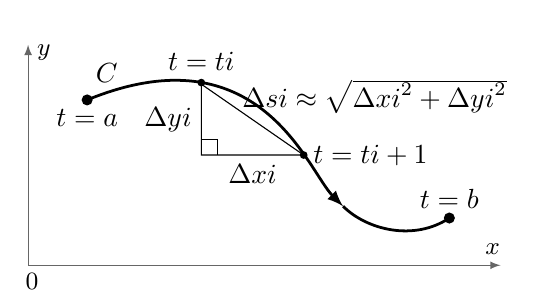
\begin{tikzpicture}
   \usetikzlibrary{arrows}
   \draw [black!60,line width=0.3pt,-latex] (0,0) -- (6,0,0);
   \draw [black!60,line width=0.3pt,-latex] (0,0) -- (0,2.8,0);
   \pgfputat{\pgfpointxyz{5.9}{0.2}{0}}{\pgfbox[center,center]{\small $x$}};
   \pgfputat{\pgfpointxyz{0.2}{2.7}{0}}{\pgfbox[center,center]{\small $y$}};
   \pgfputat{\pgfpointxyz{0.05}{-0.2}{0}}{\pgfbox[center,center]{\small $0$}};
   \draw [rounded corners,line width=1pt,-latex](0.75,2.1) .. controls (2.95,3) and (3.55,1.2) .. (4,0.75);
   \draw [rounded corners,line width=1pt] (4,0.75) .. controls (4.3,0.45) and (4.9,0.3) .. (5.35,0.6);
   \draw (2.2,2.3) -- (3.5,1.4) -- (2.2,1.4) -- (2.2,2.3);
   \draw (2.2,1.6) -- (2.4,1.6) -- (2.4,1.4);
   \node [left,above] at (1,2.2) {$C$};
   \fill (0.75,2.1) circle (2pt);
   \fill (5.35,0.6) circle (2pt);
   \fill (2.2,2.32) circle (1.4pt);
   \fill (3.5,1.4) circle (1.4pt);
   \node [below] at (0.75,2.1) {$t=a$};
   \node [above] at (5.35,0.6) {$t=b$};
   \node [right,above] at (4.4,1.8) {$\Delta \ssub{s}{i} \approx \sqrt{{\Delta\ssub{x}{i}}^2 + {\Delta\ssub{y}{i}}^2}$};
   \node [above] at (2.2,2.35) {$t=\ssub{t}{i}$};
   \node [right] at (3.5,1.4) {$t=\ssub{t}{i+1}$};
   \node [left] at (2.2,1.85) {$\Delta \ssub{y}{i}$};
   \node [below] at (2.85,1.4) {$\Delta \ssub{x}{i}$};
  \end{tikzpicture}
 \end{center}
 \caption[]{\quad Curve $C:x=x(t),y=y(t)$ for $t$ in $\ival{a}{b}$}
 \label{fig:lineintdef}
\end{figure}

We will assume for now that the function $f(x,y)$ is continuous and real-valued, so we only consider the magnitude of
the force. Partition the interval $\ival{a}{b}$ as follows:
\begin{displaymath}
 a = \ssub{t}{0} < \ssub{t}{1} < \ssub{t}{2} < \dots < \ssub{t}{n-1} < \ssub{t}{n} = b ~,~~\text{for some integer
 $n \ge 2$}
\end{displaymath}
As we can see from Figure \ref{fig:lineintdef}, over a typical subinterval $\ival{\ssub{t}{i}}{\ssub{t}{i+1}}$ the
distance $\Delta \ssub{s}{i}$ traveled along the curve is approximately $\sqrt{{\Delta\ssub{x}{i}}^2 +
{\Delta\ssub{y}{i}}^2}$, by the Pythagorean Theorem. Thus, if the subinterval is small enough then the work done in
moving the object along that piece of the curve is approximately
\begin{equation}\label{eqn:workapprox}
 \text{Force}\,\times\,\text{Distance} ~\approx~ f(\ssub{x}{i*},\ssub{y}{i*})\,\sqrt{{\Delta\ssub{x}{i}}^2 +
{\Delta\ssub{y}{i}}^2} ~,
\end{equation}
where $(\ssub{x}{i*},\ssub{y}{i*}) = (x(\ssub{t}{i}*),y(\ssub{t}{i}*))$ for some $\ssub{t}{i}*$ in
$\ival{\ssub{t}{i}}{\ssub{t}{i+1}}$, and so
\begin{equation}\label{eqn:totworkapprox}
 W ~\approx~ \sum\limits_{i=0}^{n-1} f(\ssub{x}{i*},\ssub{y}{i*})\,\sqrt{{\Delta\ssub{x}{i}}^2 +
{\Delta\ssub{y}{i}}^2}
\end{equation}
is approximately the total amount of work done over the entire curve. But since
\begin{displaymath}
 \sqrt{{\Delta\ssub{x}{i}}^2 + {\Delta\ssub{y}{i}}^2} ~=~ \sqrt{\left(\frac{\Delta\ssub{x}{i}}{\Delta\ssub{t}{i}}\right)^2
  + \left(\frac{\Delta\ssub{y}{i}}{\Delta\ssub{t}{i}}\right)^2} \,\,\Delta\ssub{t}{i} ~,
\end{displaymath}
where $\Delta\ssub{t}{i} = \ssub{t}{i+1}- \ssub{t}{i}$, then
\begin{equation}\label{eqn:totworkapprox2}
 W ~\approx~ \sum\limits_{i=0}^{n-1} f(\ssub{x}{i*},\ssub{y}{i*})\,
 \sqrt{\left(\frac{\Delta\ssub{x}{i}}{\Delta\ssub{t}{i}}\right)^2
  + \left(\frac{\Delta\ssub{y}{i}}{\Delta\ssub{t}{i}}\right)^2} \,\,\Delta\ssub{t}{i} ~.
\end{equation}
Taking the limit of that sum as the length of the largest subinterval goes to $0$, the sum over all subintervals becomes
the integral from $t=a$ to $t=b$, $\frac{\Delta\ssub{x}{i}}{\Delta\ssub{t}{i}}$ and
$\frac{\Delta\ssub{y}{i}}{\Delta\ssub{t}{i}}$ become $x\,'(t)$ and $y\,'(t)$, respectively, and
$f(\ssub{x}{i*},\ssub{y}{i*})$ becomes $f(x(t),y(t))$, so that
\begin{equation}\label{eqn:workcurvescalar}
 W ~=~ \int_a^b f(x(t),y(t)) \,\sqrt{x\,'(t)^2 + y\,'(t)^2}\,\,dt ~.
\end{equation}

The integral on the right side of the above equation gives us our idea of how to define, for \emph{any}
real-valued function $f(x,y)$, the integral of $f(x,y)$ along the curve $C$, called a \emph{line integral}:\index{line
integral}\index{$\int_C$}

\statedefn{defn:lineintscalar2}{
 For a real-valued function $f(x,y)$ and a curve $C$ in $\Real{2}$, parametrized by $x=x(t)$, $y=y(t)$, $a \le t \le b$,
 the \textbf{line integral of} $f(x,y)$ \textbf{along} $C$ \textbf{with respect to arc length} $s$ is
 \begin{equation}\label{eqn:lineintscalar}
  \int_C f(x,y)\,ds ~=~ \int_a^b f(x(t),y(t)) \,\sqrt{x\,'(t)^2 + y\,'(t)^2}\,\,dt ~.
 \end{equation}
}

The symbol $ds$ is the differential of the arc length function
\begin{equation}\label{eqn:arclen2}
 s ~=~ s(t) ~=~ \int_a^t \sqrt{x\,'(u)^2 + y\,'(u)^2}\,\,du ~,
\end{equation}
which you may recognize from Section 1.9 as the length of the curve $C$ over the interval $\ival{a}{t}$, for all
$t$ in $\ival{a}{b}$. That is,
\begin{equation}
 ds ~=~ s\,'(t)\,dt ~=~ \sqrt{x\,'(t)^2 + y\,'(t)^2}\,\,dt ~,
\end{equation}
by the Fundamental Theorem of Calculus.

For a general real-valued function $f(x,y)$, what does the line integral $\int_C f(x,y)\,ds$ represent? The preceding
discussion of $ds$ gives us a clue. You can think of differentials as infinitesimal lengths. So if you think
of $f(x,y)$ as the height of a picket fence along $C$, then $f(x,y)\,ds$ can be thought of as approximately the area of
a section of that fence over some infinitesimally small section of the curve, and thus the line integral
$\int_C f(x,y)\,ds$ is the total area of that picket fence (see Figure \ref{fig:picketfence}).

\begin{figure}[h]
 \begin{center}
  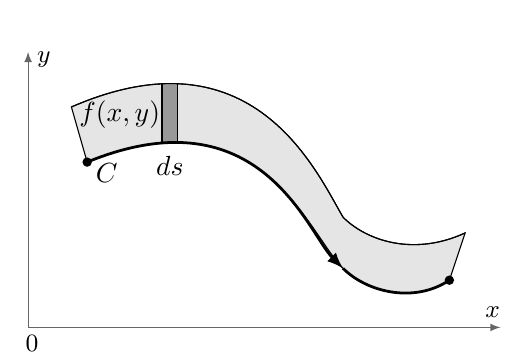
\begin{tikzpicture}
   \usetikzlibrary{arrows}
   \draw [black!60,line width=0.3pt,-latex] (0,0) -- (6,0,0);
   \draw [black!60,line width=0.3pt,-latex] (0,0) -- (0,3.5,0);
   \pgfputat{\pgfpointxyz{5.9}{0.2}{0}}{\pgfbox[center,center]{\small $x$}};
   \pgfputat{\pgfpointxyz{0.2}{3.4}{0}}{\pgfbox[center,center]{\small $y$}};
   \pgfputat{\pgfpointxyz{0.05}{-0.2}{0}}{\pgfbox[center,center]{\small $0$}};
   \filldraw [fill=black!10] (0.75,2.1) .. controls (2.95,3) and (3.55,1.2) .. (4,0.75) .. controls (4.3,0.45) and
    (4.9,0.3) .. (5.35,0.6) -- (5.55,1.2) .. controls (4.9,0.9) and (4.3,1.1) .. (4,1.4) .. controls (3.65,2) and
    (2.85,3.8) .. (0.55,2.8) -- (0.75,2.1);
   \fill [fill=black!40] (1.9,2.35) -- (1.9,3.1) -- (1.7,3.1) -- (1.7,2.35) -- (1.9,2.35);
   \draw (5.55,1.2) .. controls (4.9,0.9) and (4.3,1.1) .. (4,1.4) .. controls (3.65,2) and
    (2.85,3.8) .. (0.55,2.8);
   \draw [rounded corners,line width=1pt,-latex] (0.75,2.1) .. controls (2.95,3) and (3.55,1.2) .. (4,0.75);
   \draw [rounded corners,line width=1pt](4,0.75) .. controls (4.3,0.45) and (4.9,0.3) .. (5.35,0.6);
   \node [left,below] at (1,2.2) {$C$};
   \node [below] at (1.8,2.3) {$ds$};
   \draw (1.9,2.35) -- (1.9,3.1);
   \draw (1.7,2.35) -- (1.7,3.1);
   \node [left] at (1.8,2.7) {$f(x,y)$};
   \fill (0.75,2.1) circle (1.7pt);
   \fill (5.35,0.6) circle (1.7pt);
  \end{tikzpicture}
 \end{center}
 \caption[]{\quad Area of shaded rectangle $= \text{height}\times\text{width} \approx f(x,y)\,ds$}
 \label{fig:picketfence}
\end{figure}

\hrule width \textwidth height 0.5pt
\begin{exmp}\label{exmp:lineintcyl}
 Use a line integral to show that the lateral surface area $A$ of a right circular cylinder of radius $r$ and height $h$
 is $2\pi r h$.\smallskip
 \piccaption[]{}\parpic[r]{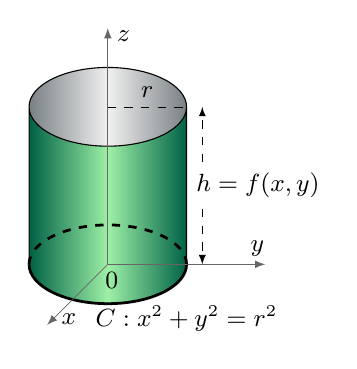
\begin{tikzpicture}
   \usetikzlibrary{arrows}
   \definecolor{insideo}{HTML}{798084}
   \definecolor{insidei}{HTML}{F0F0F0}
   \definecolor{outer}{HTML}{006146}
   \definecolor{inner}{HTML}{9EF0A6}
   \shade [left color=insideo,right color=insideo,middle color=insidei] (1,2) arc (0:180:1 and .5) --
    (-1,2) arc (180:360:1 and .5);
   \shadedraw [left color=outer,right color=outer,middle color=inner] (-1,0) arc (180:360:1 and .5) -- (1,2) --
    (1,2) arc (360:180:1 and .5) -- (-1,0);
   \draw (1,2) arc (0:180:1 and .5);
   \draw [line width=1pt] (-1,0) arc (180:360:1 and .5);
   \draw [dashed,line width=1pt] (1,0) arc (0:180:1 and .5);
   \draw [black!60,line width=0.3pt,-latex] (0,0) -- (2,0,0);
   \draw [black!60,line width=0.3pt,-latex] (0,0) -- (0,3,0);
   \draw [black!60,line width=0.3pt,-latex] (0,0) -- (0,0,2);
   \pgfputat{\pgfpointxyz{1.9}{0.2}{0}}{\pgfbox[center,center]{\small $y$}};
   \pgfputat{\pgfpointxyz{0.2}{2.9}{0}}{\pgfbox[center,center]{\small $z$}};
   \pgfputat{\pgfpointxyz{0.2}{0}{1.8}}{\pgfbox[center,center]{\small $x$}};
   \pgfputat{\pgfpointxyz{0.05}{-0.2}{0}}{\pgfbox[center,center]{\small $0$}};
   \draw [dashed,line width=0.2pt] (0,2) -- (1,2);
   \node [above] at (0.5,2) {\small $r$};
   \node [right] at (1,1) {\small $h=f(x,y)$};
   \draw [dashed,line width=0.2pt,-latex] (1.2,1.3) -- (1.2,2);
   \draw [dashed,line width=0.2pt,-latex] (1.2,0.7) -- (1.2,0);
   \node [right,below] at (1,-0.4) {\small $C: x^2 + y^2 = r^2$};
  \end{tikzpicture}}
 \par\noindent \emph{Solution:} We will use the right circular cylinder with base
 circle $C$ given by $x^2 + y^2 = r^2$ and with height $h$ in the positive $z$ direction (see Figure 4.1.3).
 Parametrize $C$ as follows:
 \begin{displaymath}
  x ~=~ x(t) ~=~ r \cos t ~,\quad y ~=~ y(t) ~=~ r \sin t~,\quad 0 \le t \le 2\pi
 \end{displaymath}
 Let $f(x,y) = h$ for all $(x,y)$. Then
 \begin{align*}
  A ~&=~ \int_C f(x,y)\,ds ~=~ \int_a^b f(x(t),y(t)) \,\sqrt{x\,'(t)^2 + y\,'(t)^2}\,\,dt\\
   &=~ \int_0^{2\pi} h \sqrt{(-r \sin t)^2 + (r \cos t)^2}\,\,dt\\
   &=~ h\int_0^{2\pi} r \sqrt{\sin^2 t + \cos^2 t}\,\,dt\\
   &=~ rh\int_0^{2\pi} 1 \,dt ~=~ 2\pi r h
 \end{align*}
\end{exmp}
\hrule width \textwidth height 0.5pt
\medskip
Note in Example \ref{exmp:lineintcyl} that if we had traversed the circle $C$ twice, i.e. let $t$ vary from $0$
to $4\pi$, then we would have gotten an area of $4\pi r h$, i.e. twice the desired area, even though the \emph{curve}
itself is still the same (namely, a circle of radius $r$). Also, notice that we traversed the circle in the
counter-clockwise direction. If we had gone in the clockwise direction, using the parametrization
\begin{equation}\label{eqn:lineintcylcwise}
 x ~=~ x(t) ~=~ r \cos (2\pi - t) ~,\quad y ~=~ y(t) ~=~ r \sin (2\pi - t)~,\quad 0 \le t \le 2\pi ~,
\end{equation}
then it is easy to verify (see Exercise 12) that the value of the line integral is unchanged.

In general, it can be shown
(see Exercise 15) that reversing the direction in which a curve $C$ is traversed leaves $\int_C f(x,y)\,ds$ unchanged,
for any $f(x,y)$. If a curve $C$ has a parametrization $x=x(t)$, $y=y(t)$, $a \le t \le b$, then denote by $-C$ the
same curve as $C$ but traversed in the opposite direction. Then $-C$ is parametrized by
\begin{equation}\label{eqn:reversec}
 x ~=~ x(a+b-t)~,\quad y ~=~ y(a+b-t)~,\quad a \le t \le b ~,
\end{equation}
and we have
\begin{equation}
 \int_C f(x,y)\,ds ~=~ \int_{-C} f(x,y)\,ds ~.
\end{equation}

Notice that our definition of the line integral was with respect to the arc length parameter $s$. We can also
define
\begin{equation}\label{eqn:lineintx2}
 \int_C f(x,y)\,dx ~=~ \int_a^b f(x(t),y(t)) \,x\,'(t)\,dt
\end{equation}
as the \emph{line integral of $f(x,y)$ along $C$ with respect to $x$}, and
\begin{equation}\label{eqn:lineinty2}
 \int_C f(x,y)\,dy ~=~ \int_a^b f(x(t),y(t)) \,y\,'(t)\,dt
\end{equation}
as the \emph{line integral of $f(x,y)$ along $C$ with respect to $y$}.

In the derivation of the formula for a line integral, we used the idea of work as force multiplied by distance.
However, we know that force is actually a \emph{vector}. So it would be helpful to develop a vector form for a
line integral. For this, suppose that we have a function $\mathbf{f}(x,y)$ defined on $\Real{2}$ by
\begin{displaymath}
 \mathbf{f}(x,y) ~=~ P(x,y)\,\mathbf{i} ~+~ Q(x,y)\,\mathbf{j}
\end{displaymath}
for some continuous real-valued functions $P(x,y)$ and $Q(x,y)$ on $\Real{2}$. Such a function $\mathbf{f}$ is called a
\textbf{vector field} on $\Real{2}$. It is defined at \emph{points} in $\Real{2}$, and its values are
\emph{vectors} in $\Real{2}$. For a curve $C$ with a smooth parametrization $x=x(t)$, $y=y(t)$, $a \le t \le b$,
let\index{vector field}
\begin{displaymath}
 \mathbf{r}(t) ~=~ x(t)\,\mathbf{i} ~+~ y(t)\,\mathbf{j}
\end{displaymath}
be the position vector for a point $(x(t),y(t))$ on $C$. Then\index{position vector}
$\mathbf{r}'(t) = x'(t)\,\mathbf{i} + y\,'(t)\,\mathbf{j}$ and so
\begin{align*}
 \int_C P(x,y)\,dx ~+~ \int_C Q(x,y)\,dy ~&=~ \int_a^b P(x(t),y(t)) \,x\,'(t)\,dt ~+~ \int_a^b Q(x(t),y(t)) \,y\,'(t)\,dt\\
  &=~ \int_a^b (P(x(t),y(t)) \,x\,'(t) + Q(x(t),y(t)) \,y\,'(t))\,dt\\
  &=~ \int_a^b \Dotprod{\mathbf{f}(x(t),y(t))}{\mathbf{r}'(t)}\,dt
\end{align*}
by definition of $\mathbf{f}(x,y)$. Notice that the function $\Dotprod{\mathbf{f}(x(t),y(t))}{\mathbf{r}\,'(t)}$
is a \emph{real-valued} function on $\ival{a}{b}$, so the last integral on the right looks somewhat similar to our
earlier definition of a line integral. This leads us to the following definition:\index{line
integral}\index{$\int_C$}

\statedefn{defn:lineintvec2}{
 For a vector field $\mathbf{f}(x,y) = P(x,y)\,\mathbf{i} + Q(x,y)\,\mathbf{j}$ and a curve $C$ with a smooth
 parametrization $x=x(t)$, $y=y(t)$, $a \le t \le b$, the \textbf{line integral of f along} $C$ is
 \begin{align}
  \int_C \Dotprod{\mathbf{f}}{d\mathbf{r}} ~&=~ \int_C P(x,y)\,dx ~+~ \int_C Q(x,y)\,dy\\
   &=~ \int_a^b \Dotprod{\mathbf{f}(x(t),y(t))}{\mathbf{r}\,'(t)}\,dt ~,
 \end{align}
 where $\mathbf{r}(t) = x(t)\,\mathbf{i} + y(t)\,\mathbf{j}$ is the position vector for points on $C$.
}
We use the notation $d\mathbf{r} = \mathbf{r}\,'(t)\,dt = dx\,\mathbf{i} + dy\,\mathbf{j}$\index{$d\mathbf{r}$} to
denote the \textbf{differential}\index{differential}
of the vector-valued function $\mathbf{r}$. The line integral in Definition \ref{defn:lineintvec2} is
often called a \emph{line integral of a vector field} to distinguish it from the line integral in
Definition \ref{defn:lineintscalar2} which is called a \emph{line integral of a scalar field}. For
convenience we will often write
\begin{displaymath}
 \int_C P(x,y)\,dx ~+~ \int_C Q(x,y)\,dy ~=~ \int_C P(x,y)\,dx + Q(x,y)\,dy ~,
\end{displaymath}
where it is understood that the line integral along $C$ is being applied to both $P$ and $Q$.
The quantity $P(x,y)\,dx + Q(x,y)\,dy$ is known as a \textbf{differential form}.\index{differential form} For a
real-valued function $F(x,y)$, the \textbf{differential} of $F$ is $dF = \frac{\partial F}{\partial x}\,dx +
\frac{\partial F}{\partial y}\,dy$. A differential form $P(x,y)\,dx + Q(x,y)\,dy$ is called \textbf{exact}\index{exact
differential form} if it equals $dF$ for some function $F(x,y)$.

Recall that if the points on a curve $C$ have position vector $\mathbf{r}(t) = x(t)\,\mathbf{i} + y(t)\,\mathbf{j}$,
then $\mathbf{r}\,'(t)$ is a tangent vector to $C$ at the point $(x(t),y(t))$ in the direction of increasing $t$
(which we call the \emph{direction of $C$}). Since $C$ is a smooth curve, then $\mathbf{r}\,'(t) \ne \mathbf{0}$ on
$\ival{a}{b}$ and hence
\begin{displaymath}
 \mathbf{T}(t) ~=~ \frac{\mathbf{r}\,'(t)}{\Norm{\mathbf{r}\,'(t)}}
\end{displaymath}
is the unit tangent vector to $C$ at $(x(t),y(t))$. Putting Definitions \ref{defn:lineintscalar2} and
\ref{defn:lineintvec2} together we get the following theorem:

\statethm{thm:lineinttangent}{
 For a vector field $\mathbf{f}(x,y) = P(x,y)\,\mathbf{i} + Q(x,y)\,\mathbf{j}$ and a curve $C$ with a smooth
 parametrization $x=x(t)$, $y=y(t)$, $a \le t \le b$ and position vector $\mathbf{r}(t) = x(t)\,\mathbf{i} +
 y(t)\,\mathbf{j}$,
 \begin{equation}\label{eqn:lineintform2}
  \int_C \Dotprod{\mathbf{f}}{d\mathbf{r}} ~=~ \int_C \Dotprod{\mathbf{f}}{\mathbf{T}}\,ds ~,
 \end{equation}
 where $\mathbf{T}(t) = \frac{\mathbf{r}\,'(t)}{\norm{\mathbf{r}\,'(t)}}$ is the unit tangent vector to $C$ at
 $(x(t),y(t))$.
}
If the vector field $\mathbf{f}(x,y)$ represents the force moving an object along a curve $C$, then the work
$W$ done by this force is
\begin{equation}\label{eqn:work}
 W ~=~ \int_C \Dotprod{\mathbf{f}}{\mathbf{T}}\,ds ~=~ \int_C \Dotprod{\mathbf{f}}{d\mathbf{r}} ~.
\end{equation}

\medskip
\hrule width \textwidth height 0.5pt
\begin{exmp}\label{exmp:lineintexmp}
 Evaluate $\int_C (x^2 + y^2 )\,dx + 2xy\,dy$, where:
 \begin{enumerate}[(a)]
  \item $C: x=t~,\quad y=2t~,\quad 0 \le t \le 1$
  \item $C: x=t~,\quad y=2t^2 ~,\quad 0 \le t \le 1$
 \end{enumerate}

 \piccaption[]{}\parpic[r]{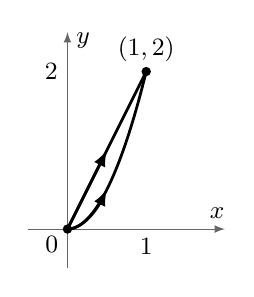
\begin{tikzpicture}
   \usetikzlibrary{arrows}
   \draw [black!60,line width=0.3pt,-latex] (-0.5,0) -- (2,0);
   \draw [black!60,line width=0.3pt,-latex] (0,-0.5) -- (0,2.5);
   \pgfputat{\pgfpointxyz{1.9}{0.2}{0}}{\pgfbox[center,center]{\small $x$}}
   \pgfputat{\pgfpointxyz{0.2}{2.4}{0}}{\pgfbox[center,center]{\small $y$}}
   \pgfputat{\pgfpointxyz{-0.2}{-0.2}{0}}{\pgfbox[center,center]{\small $0$}}
   \draw [line width=1pt] (0,0) parabola (1,2);
   \draw [line width=1pt,-latex] (0,0) parabola (0.5,0.5);
   \draw [line width=1pt] (0,0) -- (1,2);
   \draw [line width=1pt,-latex] (0,0) -- (0.5,1);
   \node [right,above] at (1,2) {\small $(1,2)$};
   \node [left] at (0,2) {\small $2$};
   \node [below] at (1,0) {\small $1$};
   \fill (0,0) circle (1.7pt);
   \fill (1,2) circle (1.7pt);
  \end{tikzpicture}}
 \par\noindent \emph{Solution:} Figure 4.1.4 shows both curves.\smallskip
 \par\noindent (a) Since $x\,'(t)=1$ and $y\,'(t)=2$, then
 \begin{align*}
  \int_C (x^2 + y^2 )\,dx + 2xy\,dy ~&=~
   \int_0^1 \left( ( x(t)^2 + y(t)^2 )x\,'(t) + 2x(t)y(t)\,y\,'(t) \right) \,dt\\
   &=~ \int_0^1 \left( (t^2 + 4t^2 )(1) + 2t(2t)(2) \right) \,dt\\
   &=~ \int_0^1 13t^2 \,dt\\
   &=~ \frac{13t^3}{3}\,\Bigg|_0^1 ~=~ \frac{13}{3}
 \end{align*}

 \par\noindent (b) Since $x\,'(t)=1$ and $y\,'(t)=4t$, then
 \begin{align*}
  \int_C (x^2 + y^2 )\,dx + 2xy\,dy ~&=~
   \int_0^1 \left( ( x(t)^2 + y(t)^2 )x\,'(t) + 2x(t)y(t)\,y\,'(t) \right) \,dt\\
   &=~ \int_0^1 \left( (t^2 + 4t^4 )(1) + 2t(2t^2 )(4t) \right) \,dt\\
   &=~ \int_0^1 (t^2 + 20t^4 )\,dt\\
   &=~ \frac{t^3}{3} + 4t^5 \,\Bigg|_0^1 ~=~ \frac{1}{3} + 4 ~=~ \frac{13}{3}
 \end{align*}

\picskip{0}
 So in both cases, if the vector field $\mathbf{f}(x,y) = ( x^2 + y^2 )\,\mathbf{i} +
 2xy\,\mathbf{j}$ represents the force moving an object from $(0,0)$ to $(1,2)$ along the given curve $C$, then the
 work done is $\frac{13}{3}$. This may lead you to think that work (and more generally, the line integral of a vector
 field) is independent of the path taken. However, as we will see in the next section, this is not always the
 case.
\end{exmp}
\hrule width \textwidth height 0.5pt
\medskip

Although we defined line integrals over a single smooth curve, if $C$ is a \emph{piecewise smooth curve}, that
is\index{piecewise smooth curve}
\begin{displaymath}
 C = \ssub{C}{1} \cup \ssub{C}{2} \cup \ldots \cup \ssub{C}{n}
\end{displaymath}
is the union of smooth curves $\ssub{C}{1},\ldots ,\ssub{C}{n}$, then we can define
\begin{displaymath}
 \int_C \Dotprod{\mathbf{f}}{d\mathbf{r}} ~=~ \int_{\ssub{C}{1}} \Dotprod{\mathbf{f}}{d\ssub{\mathbf{r}}{1}} ~+~
  \int_{\ssub{C}{2}} \Dotprod{\mathbf{f}}{d\ssub{\mathbf{r}}{2}} ~+ \ldots +~
  \int_{\ssub{C}{n}} \Dotprod{\mathbf{f}}{d\ssub{\mathbf{r}}{n}}
\end{displaymath}
where each $\ssub{\mathbf{r}}{i}$ is the position vector of the curve $\ssub{C}{i}$.

\medskip
\hrule width \textwidth height 0.5pt
\begin{exmp}\label{exmp:lineintexmppoly}
 Evaluate $\int_C (x^2 + y^2 )\,dx + 2xy\,dy$, where $C$ is the polygonal path from $(0,0)$ to $(0,2)$ to
 $(1,2)$.\smallskip

 \piccaption[]{}\parpic[r]{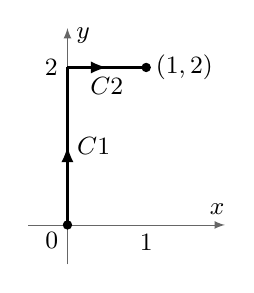
\begin{tikzpicture}
   \usetikzlibrary{arrows}
   \draw [black!60,line width=0.3pt,-latex] (-0.5,0) -- (2,0);
   \draw [black!60,line width=0.3pt,-latex] (0,-0.5) -- (0,2.5);
   \pgfputat{\pgfpointxyz{1.9}{0.2}{0}}{\pgfbox[center,center]{\small $x$}}
   \pgfputat{\pgfpointxyz{0.2}{2.4}{0}}{\pgfbox[center,center]{\small $y$}}
   \pgfputat{\pgfpointxyz{-0.2}{-0.2}{0}}{\pgfbox[center,center]{\small $0$}}
   \draw [line width=1pt] (0,0) -- (0,2);
   \draw [line width=1pt,-latex] (0,0) -- (0,1);
   \draw [line width=1pt] (0,2) -- (1,2);
   \draw [line width=1pt,-latex] (0,2) -- (0.5,2);
   \node [right] at (1,2) {\small $(1,2)$};
   \node [left] at (0,2) {\small $2$};
   \node [below] at (1,0) {\small $1$};
   \node [right] at (0,1) {\small $\ssub{C}{1}$};
   \node [below] at (0.5,2) {\small $\ssub{C}{2}$};
   \fill (0,0) circle (1.7pt);
   \fill (1,2) circle (1.7pt);
  \end{tikzpicture}}
 \par\noindent \emph{Solution:} Write $C = \ssub{C}{1} \cup \ssub{C}{2}$, where $\ssub{C}{1}$ is the curve given by
 $x=0$, $y=t$, $0 \le t \le 2$ and $\ssub{C}{2}$ is the curve given by $x=t$, $y=2$, $0 \le t \le 1$ (see Figure
 4.1.5). Then
 \begin{align*}
  \int_C (x^2 + y^2 )\,dx + 2xy\,dy ~&=~ \int_{\ssub{C}{1}} (x^2 + y^2 )\,dx + 2xy\,dy\\
   &+~ \int_{\ssub{C}{2}} (x^2 + y^2 )\,dx + 2xy\,dy\\[6pt]
   &=~ \int_0^2 \left( (0^2 + t^2 )(0) + 2(0)t(1) \right) \,dt ~+~
    \int_0^1 \left( (t^2 + 4 )(1) + 2t(2)(0) \right) \,dt\\[6pt]
   &=~ \int_0^2 0\,dt + \int_0^1 (t^2 + 4 )\,dt\\[6pt]
   &=~ \frac{t^3}{3} + 4t \,\Bigg|_0^1 ~=~ \frac{1}{3} + 4 ~=~ \frac{13}{3}
 \end{align*}
\end{exmp}
\hrule width \textwidth height 0.5pt
\medskip

Line integral notation varies quite a bit. For example, in physics it is common to see the notation
$\int_a^b \Dotprod{\mathbf{f}}{d\mathbf{l}}$, where it is understood that the limits of integration $a$ and $b$ are for
the underlying parameter $t$ of the curve, and the letter $\mathbf{l}$ signifies length. Also, the formulation
$\int_C \Dotprod{\mathbf{f}}{\mathbf{T}}\,ds$ from Theorem \ref{thm:lineinttangent} is often preferred in physics since
it emphasizes the idea of integrating the tangential component $\Dotprod{\mathbf{f}}{\mathbf{T}}$ of $\mathbf{f}$ in the
direction of $\mathbf{T}$ (i.e. in the direction of $C$), which is a useful physical interpretation of line integrals.
\hrule width \textwidth height 0.5pt
\medskip
%\startexercises
\centerline{\fbox{\textsf{\textbf{\large Exercises}}}}\label{sec4dot1}
\probs{A}
\par\noindent For Exercises 1--4, calculate 
\[\int_C f(x,y)\,ds\] for the given function $f(x,y)$ and
curve $C$.
\begin{enumerate}[\bfseries 1.]
 \item $f(x,y)=xy$; $\quad C: x=\cos t$, $y=\sin t$, $0 \le t \le \pi/2$
 \item $f(x,y)=\dfrac{x}{x^2 + 1}$; $\quad C: x=t$, $y=0$, $0 \le t \le 1$
 \item $f(x,y)=2x+y$; $\quad C$: polygonal path from $(0,0)$ to $(3,0)$ to $(3,2)$
 \item $f(x,y)=x+y^2$; $\quad C$: path from $(2,0)$ counterclockwise along the circle $x^2 + y^2 = 4$ to the point
  $(-2,0)$ and then back to $(2,0)$ along the $x$-axis
 \item Use a line integral to find the lateral surface area of the part of the cylinder\\$x^2 + y^2 = 4$ below
 the plane $x+2y+z=6$ and above the $xy$-plane.
\suspend{enumerate}
\par\noindent For Exercises 6--11, calculate 
\[\int_C \Dotprod{\mathbf{f}}{d\mathbf{r}}\] 
for the given vector
 field $\mathbf{f}(x,y)$ and curve $C$.
\resume{enumerate}[{[\bfseries 1.]}]
 \item $\mathbf{f}(x,y) = \mathbf{i} - \mathbf{j}$; $\quad C: x=3t$, $y=2t$, $0 \le t \le 1$
 \item $\mathbf{f}(x,y) = y\,\mathbf{i} - x\,\mathbf{j}$; $\quad C: x=\cos t$, $y=\sin t$, $0 \le t \le 2\pi$
 \item $\mathbf{f}(x,y) = x\,\mathbf{i} + y\,\mathbf{j}$; $\quad C: x=\cos t$, $ y=\sin t$, $0 \le t \le 2\pi$
 \item $\mathbf{f}(x,y) = (x^2 - y)\,\mathbf{i} + (x-y^2 )\,\mathbf{j}$; $\quad C: x=\cos t$, $y=\sin t$,
  $0 \le t \le 2\pi$
 \item $\mathbf{f}(x,y) = xy^2 \,\mathbf{i} + xy^3 \,\mathbf{j}$; $\quad C:$ the polygonal path from $(0,0)$ to $(1,0)$
 to $(0,1)$ to $(0,0)$
 \item $\mathbf{f}(x,y) =(x^2 + y^2 )\,\mathbf{i}$; $\quad C: x=2+\cos t$, $y=\sin t$, $0 \le t \le 2\pi$
\suspend{enumerate}
\probs{B}
\resume{enumerate}[{[\bfseries 1.]}]
 \item Verify that the value of the line integral in Example \ref{exmp:lineintcyl} is unchanged when using the
  parametrization of the circle $C$ given in formulas (\ref{eqn:lineintcylcwise}).
 \item Show that if $\mathbf{f} \perp \mathbf{r}\,'(t)$ at each point $\mathbf{r}(t)$ along a smooth curve $C$, then
  \[\int_C \Dotprod{\mathbf{f}}{d\mathbf{r}} = 0.\]
 \item Show that if $\mathbf{f}$ points in the same direction as $\mathbf{r}\,'(t)$ at each point $\mathbf{r}(t)$ along
  a smooth curve $C$, then 
  \[\int_C \Dotprod{\mathbf{f}}{d\mathbf{r}} = \int_C \norm{\mathbf{f}}\,ds.\]
\suspend{enumerate}
\probs{C}
\resume{enumerate}[{[\bfseries 1.]}]
 \item Prove that \[\int_C f(x,y)\,ds = \int_{-C} f(x,y)\,ds.\] 
 (\emph{Hint: Use formulas (\ref{eqn:reversec}).})
 \item Let $C$ be a smooth curve with arc length $L$, and suppose that $\mathbf{f}(x,y) = P(x,y)\,\mathbf{i} +
  Q(x,y)\,\mathbf{j}$ is a vector field such that $\norm{\mathbf{f}(x,y)} \le M$ for all $(x,y)$ on $C$. Show
  that
  \[\Abs{\int_C \Dotprod{\mathbf{f}}{d\mathbf{r}}} \le ML.\]
  (\emph{Hint: Recall that $\Abs{\int_a^b g(x)\,dx} \le \int_a^b \abs{g(x)}\,dx$ for Riemann integrals.})
 \item Prove that the Riemann integral $\int_a^b f(x)\,dx$ is a special case of a line integral.
\end{enumerate}
\newpage
%Begin Section 4.2
\section{Properties of Line Integrals}
We know from the previous section that for line integrals of real-valued functions (scalar fields), reversing the
direction in which the integral is taken along a curve does not change the value of the line integral:
\begin{equation}
 \int_C f(x,y)\,ds = \int_{-C} f(x,y)\,ds
\end{equation}
For line integrals of vector fields, however, the value does change. To see this, let $\mathbf{f}(x,y) =
P(x,y)\,\mathbf{i} + Q(x,y)\,\mathbf{j}$ be a vector field, with $P$ and $Q$ continuously differentiable
functions. Let $C$ be a smooth curve parametrized by $x=x(t)$, $y=y(t)$, $a \le t \le b$, with position vector
$\mathbf{r}(t) = x(t)\,\mathbf{i} + y(t)\,\mathbf{j}$ (we will usually abbreviate this by saying that
$C: \mathbf{r}(t) = x(t)\,\mathbf{i} + y(t)\,\mathbf{j}$ is a smooth curve). We know that the curve $-C$ traversed in
the opposite direction is parametrized by $x=x(a+b-t)$, $y=y(a+b-t)$, $a \le t \le b$. Then
\begin{align*}
 \int_{-C} P(x,y)\,dx ~&=~ \int_a^b P(x(a+b-t),y(a+b-t))\,\frac{d}{dt}(x(a+b-t))\,dt\\
  &=~ \int_a^b P(x(a+b-t),y(a+b-t))\,(-x\,'(a+b-t))\,dt~~\text{(by the Chain Rule)}\\
  &=~ \int_b^a P(x(u),y(u))\,(-x\,'(u))\,(-du)~~\text{(by letting $u=a+b-t$)}\\
  &=~ \int_b^a P(x(u),y(u))\,x\,'(u)\,du\\
  &=~ -\int_a^b P(x(u),y(u))\,x\,'(u)\,du~,~~\text{since $\int_b^a = -\int_a^b ~~$, so}\\
  \int_{-C} P(x,y)\,dx ~&=~ -\int_C P(x,y)\,dx
\end{align*}
since we are just using a different letter ($u$) for the line integral along $C$. A similar argument shows that
\begin{displaymath}
 \int_{-C} Q(x,y)\,dy ~=~ -\int_C Q(x,y)\,dy ~,
\end{displaymath}
and hence
\begin{align}
 \int_{-C} \Dotprod{\mathbf{f}}{d\mathbf{r}} ~&=~ \int_{-C} P(x,y)\,dx + \int_{-C} Q(x,y)\,dy\notag\\
  &=~ -\int_C P(x,y)\,dx + -\int_C Q(x,y)\,dy\notag\\
  &=~ -\left( \int_C P(x,y)\,dx + \int_C Q(x,y)\,dy \right)\notag\\
  \int_{-C} \Dotprod{\mathbf{f}}{d\mathbf{r}} ~&=~ -\int_C \Dotprod{\mathbf{f}}{d\mathbf{r}} ~.
\end{align}

The above formula can be interpreted in terms of the work done by a force $\mathbf{f}(x,y)$ (treated as a vector) moving
an object along a curve $C$: the total work performed moving the object along $C$ from its initial point to its terminal
point, and then back to the initial point moving backwards along the same path, is zero. This is because when force is
considered as a vector, direction is accounted for.

The preceding discussion shows the importance of always taking the \emph{direction} of the curve into account when
using line integrals of vector fields. For this reason, the curves in line integrals are sometimes referred to as
\emph{directed curves} or \emph{oriented curves}.\index{directed curve}

Recall that our definition of a line integral required that we have
\emph{a} parametrization $x=x(t)$, $y=y(t)$, $a \le t \le b$ for the curve $C$. But as we know, any curve has
infinitely many parametrizations. So could we get a different value for a
line integral using some other parametrization of $C$, say, $x=\tilde{x}(u)$, $y=\tilde{y}(u)$, $c \le u \le d$ ? If so,
this would mean that our definition is not well-defined. Luckily, it turns out that the value of a line
integral of a vector field is unchanged as long as the direction of the curve $C$ is preserved by whatever
parametrization is chosen:

\statethm{thm:lineintreparam}{
 {Let $\mathbf{f}(x,y) = P(x,y)\,\mathbf{i} + Q(x,y)\,\mathbf{j}$ be a vector field, and let $C$ be a smooth
 curve parametrized by $x=x(t)$, $y=y(t)$, $a \le t \le b$. Suppose that $t=\alpha(u)$ for $c \le u \le d$, such that
 $a=\alpha(c)$, $b=\alpha(d)$, and $\alpha\,'(u) > 0$ on the open interval $(c,d)$ (i.e. $\alpha(u)$ is strictly
 increasing on $\ival{c}{d}$). Then $\int_C \Dotprod{\mathbf{f}}{d\mathbf{r}}$ has the same value for the
 parametrizations $x=x(t)$, $y=y(t)$, $a \le t \le b$ and $x=\tilde{x}(u)=x(\alpha(u))$, $y=\tilde{y}(u)=y(\alpha(u))$,
 $c \le u \le d$.}
}
\begin{proofbar}\begin{proof}[Proof:]
 Since $\alpha(u)$ is strictly increasing and maps $\ival{c}{d}$ onto $\ival{a}{b}$, then we know that $t=\alpha(u)$ has
 an inverse function $u=\alpha^{-1}(t)$ defined on $\ival{a}{b}$ such that $c=\alpha^{-1}(a)$,
 $d=\alpha^{-1}(b)$, and $\frac{du}{dt} = \frac{1}{\alpha\,'(u)}$. Also, $dt = \alpha\,'(u)\,du$, and by the Chain Rule
 \begin{displaymath}
  \tilde{x}\,'(u) ~=~ \frac{d\tilde{x}}{du} ~=~ \frac{d}{du}(x(\alpha(u))) ~=~ \frac{dx}{dt}\,\frac{dt}{du} ~=~
  x\,'(t)\,\alpha\,'(u) \quad\Rightarrow\quad x\,'(t) ~=~ \frac{\tilde{x}\,'(u)}{\alpha\,'(u)}
 \end{displaymath}
 so making the susbstitution $t=\alpha(u)$ gives
 \begin{align*}
  \int_a^b P(x(t),y(t))\,x\,'(t)\,dt ~&=~
   \int_{\alpha^{-1}(a)}^{\alpha^{-1}(b)} P(x(\alpha(u)),y(\alpha(u)))\,\frac{\tilde{x}\,'(u)}{\alpha\,'(u)}
   \,(\alpha\,'(u)\,du)\\
   &=~ \int_c^d P(\tilde{x}(u),\tilde{y}(u))\,\tilde{x}\,'(u)\,du ~,
 \end{align*}
 which shows that $\int_C P(x,y)\,dx$ has the same value for both parametrizations. A similar argument shows that
 $\int_C Q(x,y)\,dy$ has the same value for both parametrizations, and hence $\int_C \Dotprod{\mathbf{f}}{d\mathbf{r}}$
 has the same value.
 
\end{proof}\end{proofbar}

Notice that the condition $\alpha\,'(u) > 0$ in Theorem \ref{thm:lineintreparam} means that the two parametrizations
move along $C$ in the same direction. That was \emph{not} the case with the ``reverse'' parametrization for $-C$: for
$u=a+b-t$ we have $t=\alpha(u)=a+b-u \Rightarrow \alpha\,'(u) = -1 <0$.

\begin{exmp}
 Evaluate the line integral $\int_C (x^2 + y^2 )\,dx + 2xy\,dy$ from Example \ref{exmp:lineintexmp}, Section 4.1, along
 the curve $C: x=t$, $y=2t^2$, $0 \le t \le 1$, where $t=\sin u$ for $0 \le u \le \pi/2$.\smallskip
 \par\noindent \emph{Solution:} First, we notice that $0=\sin 0$, $1=\sin (\pi/2)$, and $\frac{dt}{du} = \cos u > 0$ on
 $(0,\pi/2)$. So by Theorem \ref{thm:lineintreparam} we know that if $C$ is parametrized by
 \begin{displaymath}
  x=\sin u ~,\quad y = 2\sin^2 u ~,\quad 0 \le u \le \pi/2
 \end{displaymath}
 then $\int_C (x^2 + y^2 )\,dx + 2xy\,dy$ should have the same value as we found in Example \ref{exmp:lineintexmp},
 namely $\frac{13}{3}$. And we can indeed verify this:
 \begin{align*}
  \int_C (x^2 + y^2 )\,dx + 2xy\,dy ~&=~ \int_0^{\pi/2} \left( (\sin^2 u + (2\sin^2 u)^2) \cos u +
   2(\sin u)(2\sin^2 u) 4\sin u \, \cos u \right)\,du\\
   &=~ \int_0^{\pi/2} \left( \sin^2 u + 20\sin^4 u \right) \cos u\,du\\
   &=~ \frac{\sin^3 u}{3} + 4\sin^5 u \,\Bigg|_0^{\pi/2}\\
   &=~ \frac{1}{3} + 4 ~=~ \frac{13}{3}
 \end{align*}
 In other words, the line integral is unchanged whether $t$ or $u$ is the parameter for $C$.
\end{exmp}
\hrule width \textwidth height 0.5pt
\medskip

By a \textbf{closed curve}, we mean a curve $C$ whose initial point and terminal point are the same, i.e. for $C:$
$x=x(t)$, $y=y(t)$, $a \le t \le b$, we have $(x(a),y(a)) = (x(b),y(b))$.\index{closed curve}

\begin{figure}[h]
 \centering
 \subfloat[][Closed]{
 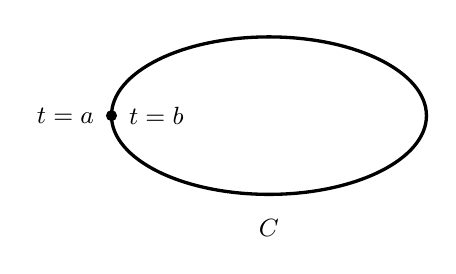
\begin{tikzpicture}
  \usetikzlibrary{arrows}
  \fill (-2,0) circle (2pt);
  \draw [black,line width=1.2pt] (-2,0) arc (180:90:2 and 1) node {\large $\blacktriangleright$};
  \draw [black,line width=1.2pt] (0,1) arc (90:-90:2 and 1) node {\large $\blacktriangleleft$};
  \draw [black,line width=1.2pt] (0,-1) arc (-90:-180:2 and 1);
  \node [below] at (0,-1.2) {\small $C$};
  \node [left] at (-2.1,0) {\small $t=a$};
  \node [right] at (-1.9,0) {\small $t=b$};
 \end{tikzpicture}}
 \qquad\qquad
 \subfloat[][Not closed]{
 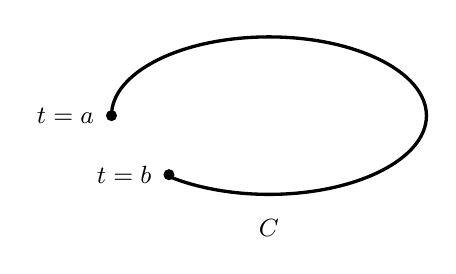
\begin{tikzpicture}
  \usetikzlibrary{arrows}
  \fill (-2,0) circle (2pt);
  \fill (-1.27,-0.75) circle (2pt);
  \draw [black,line width=1.2pt] (-2,0) arc (180:90:2 and 1) node {\large $\blacktriangleright$};
  \draw [black,line width=1.2pt] (0,1) arc (90:-90:2 and 1) node {\large $\blacktriangleleft$};
  \draw [black,line width=1.2pt] (0,-1) arc (-90:-130:2 and 1);
  \node [below] at (0,-1.2) {\small $C$};
  \node [left] at (-2.1,0) {\small $t=a$};
  \node [left] at (-1.37,-0.75) {\small $t=b$};
 \end{tikzpicture}}
 \caption[]{\quad Closed vs nonclosed curves}
 \label{fig:closedcurve}
\end{figure}

A \textbf{simple closed curve} is a closed curve which does not intersect itself. Note that any closed curve can be
regarded as a union of simple closed curves (think of the loops in a figure eight). We use the special notation
\begin{displaymath}
 \oint_C f(x,y)\,ds \quad\text{and}\quad \oint_C \Dotprod{\mathbf{f}}{d\mathbf{r}}
\end{displaymath}
to denote line integrals of scalar and vector fields, respectively, along closed curves.\index{simple closed
curve}\index{$\oint_C$} In some older texts you may see the notation $\;\displaystyle\counterint\;$ or
$\;\displaystyle\clockint\;$ to indicate a line integral traversing a closed curve in a counterclockwise or
clockwise direction, respectively.

So far, the examples we have seen of line integrals (e.g. Example \ref{exmp:lineintexmp}) have had the same value
for different curves joining the initial point to the terminal point. That is, the line integral has been
independent of the path joining the two points. As we mentioned before, this is not always the case. The following
theorem gives a necessary and sufficient condition for this \emph{path independence}:\index{path
independence}

\statethm{thm:lineintpathindep}{
 {In a region $R$, the line integral $\lineintvec{C}{f}{r}$ is independent of the path between any two points in $R$
  if and only if $\olineintvec{C}{f}{r} = 0$ for every closed curve $C$ which is contained in $R$.}
}
\begin{proofbar}\begin{proof}[Proof:]
 Suppose that $\olineintvec{C}{f}{r} = 0$ for every closed curve $C$  which is contained in $R$. Let $\ssub{P}{1}$ and
 $\ssub{P}{2}$ be two distinct points in $R$. Let $\ssub{C}{1}$ be a curve in $R$ going from
 $\ssub{P}{1}$ to $\ssub{P}{2}$, and let $\ssub{C}{2}$ be another curve in $R$ going from $\ssub{P}{1}$ to
 $\ssub{P}{2}$, as in Figure 4.2.2.
 
 \piccaption[]{}\parpic[r]{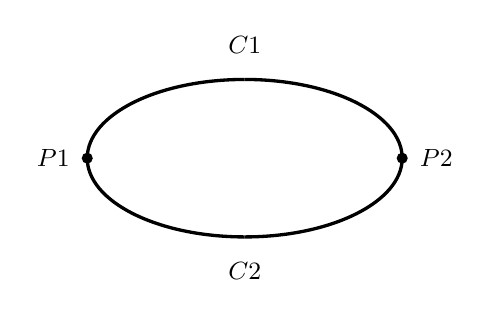
\begin{tikzpicture}
  \usetikzlibrary{arrows}
  \fill (-2,0) circle (2pt);
  \fill (2,0) circle (2pt);
  \draw [black,line width=1.2pt] (-2,0) arc (180:90:2 and 1) node {\large $\blacktriangleright$};
  \draw [black,line width=1.2pt] (0,1) arc (90:-90:2 and 1) node {\large $\blacktriangleright$};
  \draw [black,line width=1.2pt] (0,-1) arc (-90:-180:2 and 1);
  \node [above] at (0,1.2) {\small $\ssub{C}{1}$};
  \node [below] at (0,-1.2) {\small $\ssub{C}{2}$};
  \node [left] at (-2.1,0) {\small $\ssub{P}{1}$};
  \node [right] at (2.1,0) {\small $\ssub{P}{2}$};
 \end{tikzpicture}}
 \par Then $C = \ssub{C}{1} \cup \ssub{-C}{2}$ is a closed curve in $R$ (from
 $\ssub{P}{1}$ to $\ssub{P}{1}$), and so $\olineintvec{C}{f}{r} = 0$. Thus,
 \begin{align*}
  0 ~&=~ \olineintvec{C}{f}{r}\\[6pt]
   &=~ \lineintvec{\ssub{C}{1}}{f}{r} ~+~ \lineintvec{\ssub{-C}{2}}{f}{r}\\[6pt]
   &=~ \lineintvec{\ssub{C}{1}}{f}{r} ~-~ \lineintvec{\ssub{C}{2}}{f}{r}~,~\text{and so}
 \end{align*}
 $\lineintvec{\ssub{C}{1}}{f}{r} = \lineintvec{\ssub{C}{2}}{f}{r}$. This proves path independence.

 \picskip{0}
 \par
 Conversely, suppose that the line integral $\lineintvec{C}{f}{r}$ is independent of the path
 between any two points in $R$. Let $C$ be a closed curve contained in $R$. Let $\ssub{P}{1}$ and $\ssub{P}{2}$ be two
 distinct points on $C$. Let $\ssub{C}{1}$ be a part of the curve $C$ that goes from $\ssub{P}{1}$ to $\ssub{P}{2}$, and
 let $\ssub{C}{2}$ be the remaining part of $C$ that goes from $\ssub{P}{1}$ to $\ssub{P}{2}$, again as in Figure 4.2.2.
 Then by path independence we have
 \begin{align*}
  \lineintvec{\ssub{C}{1}}{f}{r} ~&=~ \lineintvec{\ssub{C}{2}}{f}{r}\\[6pt]
  \lineintvec{\ssub{C}{1}}{f}{r} ~-~ \lineintvec{\ssub{C}{2}}{f}{r} ~&=~ 0\\[6pt]
  \lineintvec{\ssub{C}{1}}{f}{r} ~+~ \lineintvec{\ssub{-C}{2}}{f}{r} ~&=~ 0 ~,~\text{so}\\[6pt]
  \olineintvec{C}{f}{r} ~&=~ 0
 \end{align*}
 since $C = \ssub{C}{1} \cup \ssub{-C}{2}$ . \qedhere
 
\end{proof}\end{proofbar}

Clearly, the above theorem does not give a practical way to determine path independence, since it is impossible to
check the line integrals around all possible closed curves in a region.
What it mostly does is give an idea of the
way in which line integrals behave, and how seemingly unrelated line integrals can be related (in this case, a
specific line integral between two points and \emph{all} line integrals around closed curves).

Recall that if $z=f(x,y)$ is a continuously differentiable function of $x$ and $y$, and both $x=x(t)$ and $y=y(t)$ are
 differentiable functions of $t$, then 
 \begin{equation}\label{eqn:chainrule2}
  \frac{dz}{dt} ~=~ \frac{\partial z}{\partial x}\,\frac{dx}{dt} ~+~ \frac{\partial z}{\partial y}\,\frac{dy}{dt}.
 \end{equation}
This is multivariable version of the Chain Rule, see Theorem \ref{thm:multichain} and Corollary \ref{cor:dirderiv}.
We will now use this version of Chain Rule to prove the
following \emph{sufficient} condition for path independence of line integrals:

\statethm{thm:lineintsuffpath}{
 {Let $\mathbf{f}(x,y) = P(x,y)\,\mathbf{i} + Q(x,y)\,\mathbf{j}$ be a vector field in some region $R$, with $P$
 and $Q$ continuously differentiable functions on $R$. Let $C$ be a smooth curve in $R$ parametrized by $x=x(t)$,
 $y=y(t)$, $a \le t \le b$. Suppose that there is a real-valued function $F(x,y)$ such that $\nabla F = \mathbf{f}$ on
 $R$. Then
 \begin{equation}\label{eqn:lineintsuffpath}
  \lineintvec{C}{f}{r} ~=~ F(B) ~-~ F(A) ~,
 \end{equation}
 where $A=(x(a),y(a))$ and $B=(x(b),y(b))$ are the endpoints of $C$. Thus, the line integral is independent of the path
 between its endpoints, since it depends only on the values of $F$ at those endpoints.}
}
\begin{proofbar}\begin{proof}[Proof:]
 By definition of $\lineintvec{C}{f}{r}$, we have
 \begin{align*}
  \lineintvec{C}{f}{r} ~&=~ \int_a^b \left( P(x(t),y(t))\,x\,'(t) + Q(x(t),y(t))\,y\,'(t) \right)\,dt\\
   &=~ \int_a^b \left( \frac{\partial F}{\partial x}\,\frac{dx}{dt} + \frac{\partial F}{\partial y}\,\frac{dy}{dt}
   \right)\,dt ~~\text{(since $\nabla F = \mathbf{f} ~\Rightarrow~ \frac{\partial F}{\partial x} = P$ and
   $\frac{\partial F}{\partial y} = Q$)}\\
   &=~ \int_a^b F(x(t),y(t))'\,dt ~~\text{(by the Chain Rule in Theorem \ref{thm:multichain})}\\
   &=~ F(x(t),y(t)) \,\Big|_a^b ~=~ F(B) ~-~ F(A)
 \end{align*}
 by the Fundamental Theorem of Calculus.
 
\end{proof}\end{proofbar}

Theorem \ref{thm:lineintsuffpath} can be thought of as the line integral version of the Fundamental Theorem of
Calculus. A real-valued function $F(x,y)$ such that $\nabla F(x,y) = \mathbf{f}(x,y)$ is called a \textbf{potential} for $\mathbf{f}$. 
A \textbf{conservative} vector field is one which has a potential.\index{potential}

\medskip
\hrule width \textwidth height 0.5pt
\begin{exmp}\label{exmp:lineintexmpclosed}
 Recall from Examples \ref{exmp:lineintexmp}  and \ref{exmp:lineintexmppoly} in Section 4.1 that the line
 integral $\int_C (x^2 + y^2 )\,dx + 2xy\,dy$ was found to have the value $\frac{13}{3}$ for three different curves $C$
 going from the point $(0,0)$ to the point $(1,2)$. Use Theorem \ref{thm:lineintsuffpath} to show that this line
 integral is indeed path independent.\smallskip
 \par\noindent \emph{Solution:} We need to find a real-valued function $F(x,y)$ such that
 \begin{displaymath}
  \frac{\partial F}{\partial x} = x^2 + y^2 \quad\text{and}\quad \frac{\partial F}{\partial y} =  2xy ~.
 \end{displaymath}
 Suppose that $\frac{\partial F}{\partial x} = x^2 + y^2$, Then we must have $F(x,y) = \frac{1}{3}x^3 + xy^2 + g(y)$ for
 some function $g(y)$. So $\frac{\partial F}{\partial y} = 2xy + g\,'(y)$
 satisfies the condition $\frac{\partial F}{\partial y} = 2xy$ if $g\,'(y)=0$, i.e. $g(y)=K$, where $K$ is a
 constant. Since any choice for $K$ will do (why?), we pick $K=0$. Thus, a potential $F(x,y)$ for 
 $\mathbf{f}(x,y) = ( x^2 + y^2 )\,\mathbf{i} + 2xy\,\mathbf{j}$ exists, namely
 \begin{displaymath}
  F(x,y) ~=~ \frac{1}{3}x^3 + xy^2 ~.
 \end{displaymath}
 Hence the line integral $\int_C (x^2 + y^2 )\,dx + 2xy\,dy$ is path independent.\index{conservative field}
 
 \par\noindent Note that we can also verify that the value of the line integral of $\mathbf{f}$ along any curve $C$ going
 from $(0,0)$ to $(1,2)$ will always be $\frac{13}{3}$, since by Theorem \ref{thm:lineintsuffpath}
 \begin{displaymath}
  \lineintvec{C}{f}{r} ~=~ F(1,2) ~-~ F(0,0) ~=~ \frac{1}{3}(1)^3 + (1)(2)^2 - (0+0) ~=~ \frac{1}{3} + 4 ~=~ \frac{13}{3} ~.
 \end{displaymath}
\end{exmp}
\hrule width \textwidth height 0.5pt
\medskip

A consequence of Theorem \ref{thm:lineintsuffpath} in the special case where $C$ is a closed curve, so that the
endpoints $A$ and $B$ are the same point, is the following important corollary:

\statecor{cor:lineintsuffpath}{
 {If a vector field $\mathbf{f}$ has a potential in a region $R$, then $\displaystyle\olineintvec{C}{f}{r} = 0$
 for any closed curve $C$ in $R$ (i.e. $\displaystyle\oint_{C}\Dotprod{\nabla F}{d\mathbf{r}} = 0$ for any real-valued
 function $F(x,y)$).}
}

\medskip
\hrule width \textwidth height 0.5pt
\begin{exmp}
 Evaluate $\displaystyle\oint_C x\,dx + y\,dy$ for $C:$ $x=2\cos t$, $y=3\sin t$,
 $0\le t\le 2\pi$.\smallskip
 \par\noindent \emph{Solution:} The vector field $\mathbf{f}(x,y) = x\,\mathbf{i} + y\,\mathbf{j}$ has a
 potential $F(x,y)$:
 \begin{align*}
  \frac{\partial F}{\partial x} = x ~&\Rightarrow~ F(x,y) ~=~ \frac{1}{2}x^2 + g(y) ~,\text{so}\\
  \frac{\partial F}{\partial y} = y ~&\Rightarrow~ g\,'(y) = y ~\Rightarrow~ g(y) ~=~ \frac{1}{2}y^2 + K
 \end{align*}
 for any constant $K$, so $F(x,y) = \dfrac{1}{2}x^2 + \dfrac{1}{2}y^2$ is a potential for $\mathbf{f}(x,y)$. Thus,
 \begin{displaymath}
  \displaystyle\oint_C x\,dx + y\,dy ~=~ \displaystyle\olineintvec{C}{f}{r} ~=~ 0
 \end{displaymath}
 by Corollary \ref{cor:lineintsuffpath}, since the curve $C$ is closed (it is the ellipse
 $\frac{x^2}{4}+\frac{y^2}{9}=1$).
\end{exmp}
\startexercises\label{sec4dot2}
\probs{A}
\begin{enumerate}[\bfseries 1.]
 \item Evaluate $\displaystyle\oint_C (x^2 + y^2 )\,dx + 2xy\,dy$ for $C:$ $x=\cos t$, $y=\sin t$, $0\le t\le 2\pi$.
 \item Evaluate $\displaystyle\int_C (x^2 + y^2 )\,dx + 2xy\,dy$ for $C:$ $x=\cos t$, $y=\sin t$, $0\le t\le \pi$.
 \item Is there a potential $F(x,y)$ for $\mathbf{f}(x,y) = y\,\mathbf{i} - x\,\mathbf{j}$? If so, find one.
 \item Is there a potential $F(x,y)$ for $\mathbf{f}(x,y) = x\,\mathbf{i} - y\,\mathbf{j}$? If so, find one.
 \item Is there a potential $F(x,y)$ for $\mathbf{f}(x,y) = xy^2\,\mathbf{i} + x^3 y\,\mathbf{j}$? If so, find
  one.
\suspend{enumerate}
\probs{B}
\resume{enumerate}[{[\bfseries 1.]}]
 \item Let $\mathbf{f}(x,y)$ and $\mathbf{g}(x,y)$ be vector fields, let $a$ and $b$ be constants, and let $C$ be
  a curve in $\Real{2}$. Show that
  \begin{displaymath}
   \int_{C}\Dotprod{(a\,\mathbf{f} \pm b\,\mathbf{g})}{d\mathbf{r}} ~=~ a \int_{C}\Dotprod{\mathbf{f}}{d\mathbf{r}} ~\pm~
   b \int_{C}\Dotprod{\mathbf{g}}{d\mathbf{r}} ~.
  \end{displaymath}
 \item Let $C$ be a curve whose arc length is $L$. Show that $\int_C 1\,ds = L$.
 \item Let $f(x,y)$ and $g(x,y)$ be continuously differentiable real-valued functions in a region $R$. Show that
  \begin{displaymath}
   \oint_{C}\Dotprod{f\,\nabla g}{d\mathbf{r}} ~=~ -\oint_{C}\Dotprod{g\,\nabla f}{d\mathbf{r}}
  \end{displaymath}
  for any closed curve $C$ in $R$. (\emph{Hint: Use Exercise 21 in Section 2.4.})
 \item Let $\mathbf{f}(x,y)=\frac{-y}{x^2 + y^2}\,\mathbf{i} + \frac{x}{x^2 + y^2}\,\mathbf{j}$ for all $(x,y)\ne(0,0)$,
  and $C:$ $x=\cos t$, $y=\sin t$, $0\le t\le 2\pi$.
  \begin{enumerate}[(a)]
   \item Show that \[\mathbf{f} = \nabla F,\] for $F(x,y) = \tan^{-1}(y/x)$.
   \item Show that \[\olineintvec{C}{f}{r} = 2\pi.\] Does this contradict Corollary
    \ref{cor:lineintsuffpath}? Explain.
  \end{enumerate}
\suspend{enumerate}
\probs{C}
\resume{enumerate}[{[\bfseries 1.]}]
 \item Let $g(x)$ and $h(y)$ be differentiable functions, and let $\mathbf{f}(x,y)=h(y)\,\mathbf{i} + g(x)\,\mathbf{j}$.
  Can $\mathbf{f}$ have a potential $F(x,y)$? If so, find it. You may assume that $F$ would be smooth. (\emph{Hint:
  Consider the mixed partial derivatives of $F$.})
\end{enumerate}
\newpage
%Begin Section 4.3
\section{Green's Theorem}
We will now see a way of evaluating the line integral of a \emph{smooth} vector field
around a simple closed curve. 
A vector field $\mathbf{f}(x,y) = P(x,y)\,\mathbf{i} + Q(x,y)\,\mathbf{j}$ is \textbf{smooth} if its
component functions $P(x,y)$ and $Q(x,y)$ are smooth.\index{vector field!smooth}
We will use
\emph{Green's Theorem} (sometimes called \emph{Green's Theorem in the plane}) to relate the \emph{line} integral around
a closed curve with a \emph{double} integral over the region inside the curve:\index{Green's Theorem}

\statethm{thm:green}{
 {(\textbf{Green's Theorem})
  Let $R$ be a region in $\Real{2}$ whose boundary is a simple closed curve $C$ which is piecewise smooth.
  Let $\mathbf{f}(x,y) = P(x,y)\,\mathbf{i} + Q(x,y)\,\mathbf{j}$ be a smooth vector field defined on both
  $R$ and $C$. Then
  \begin{equation}\label{eqn:green}
   \olineintvec{C}{f}{r} ~=~ \iint\limits_{R} \left( \frac{\partial Q}{\partial x} - \frac{\partial P}{\partial y} \right)
   \,dA ~,
  \end{equation}
  where $C$ is traversed so that $R$ is always on the left side of $C$.}
}
\begin{proofbar}\begin{proof}[Proof:]
 We will prove the theorem in the case for a \emph{simple} region $R$, that is, where the boundary curve $C$ can be
 written as $C = \ssub{C}1 \cup \ssub{C}{2}$ in two distinct ways:
 \begin{align}
  \ssub{C}{1} &= \text{the curve $y = \ssub{y}{1}(x)$ from the point $\ssub{X}{1}$ to the point $\ssub{X}{2}$}\\
  \ssub{C}{2} &= \text{the curve $y = \ssub{y}{2}(x)$ from the point $\ssub{X}{2}$ to the point $\ssub{X}{1}$,}
 \end{align}
 where $\ssub{X}{1}$ and $\ssub{X}{2}$ are the points on $C$ farthest to the left and right, respectively; and
 \begin{align}
  \ssub{C}{1} &= \text{the curve $x = \ssub{x}{1}(y)$ from the point $\ssub{Y}{2}$ to the point $\ssub{Y}{1}$}\\
  \ssub{C}{2} &= \text{the curve $x = \ssub{x}{2}(y)$ from the point $\ssub{Y}{1}$ to the point $\ssub{Y}{2}$,}
 \end{align}
 where $\ssub{Y}{1}$ and $\ssub{Y}{2}$ are the lowest and highest points, respectively, on $C$.
 See Figure 4.3.1.
 \piccaption[]{}\parpic(\textwidth,0in){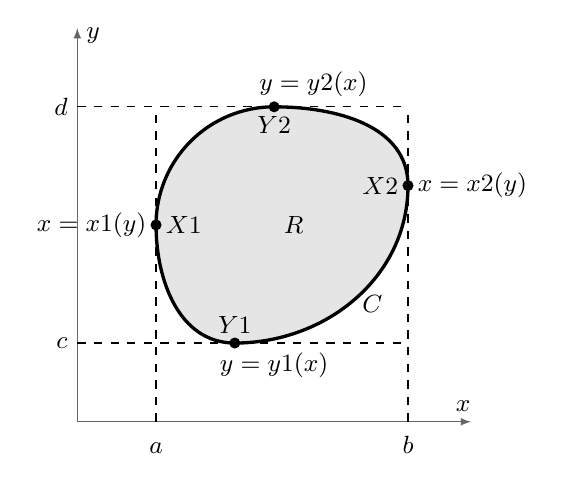
\begin{tikzpicture}
  \usetikzlibrary{arrows}
  \draw [black!60,line width=0.3pt,-latex,anchor=base] (0,0) -- (5,0)
    node[black,shift={(0,-0.4)}] at (1,0) {\small $a$}
    node[black,shift={(0,-0.4)}] at (4.2,0) {\small $b$};
  \draw [black!60,line width=0.3pt,-latex] (0,0) -- (0,5);
  \pgfputat{\pgfpointxyz{4.9}{0.2}{0}}{\pgfbox[center,center]{\small $x$}}
  \pgfputat{\pgfpointxyz{0.2}{4.9}{0}}{\pgfbox[center,center]{\small $y$}}
  \filldraw [black,line width=1.2pt,fill=black!10] (1,2.5) to[out=90,in=180] node [sloped]
  {\large $\blacktriangleleft$} (2.5,4) to[out=0,in=90] (4.2,3) to[out=270,in=0] node [sloped]
  {\large $\blacktriangleright$}(2,1) to[out=180,in=270] (1,2.5);
  \node [above] at (3,4) {\small $y = \ssub{y}{2}(x)$};
  \node [below] at (2.5,1) {\small $y = \ssub{y}{1}(x)$};
  \node [right] at (4.2,3) {\small $x = \ssub{x}{2}(y)$};
  \node [left] at (1,2.5) {\small $x = \ssub{x}{1}(y)$};
  \node [below] at (2.5,4) {\small $\ssub{Y}{2}$};
  \node [above] at (2,1) {\small $\ssub{Y}{1}$};
  \node [left] at (4.2,3) {\small $\ssub{X}{2}$};
  \node [right] at (1,2.5) {\small $\ssub{X}{1}$};
  \node [right] at (2.5,2.5) {\small $R$};
  \node [left] at (4,1.5) {\small $C$};
  \draw [dashed] (1,0) -- (1,4);
  \draw [dashed] (4.2,0) -- (4.2,4);
  \draw [dashed] (0,4) -- (4.2,4);
  \draw [dashed] (0,1) -- (4.2,1);
  \node [left] at (0,4) {\small $d$};
  \node [left] at (0,1) {\small $c$};
  \fill (1,2.5) circle (2pt);
  \fill (2.5,4) circle (2pt);
  \fill (4.2,3) circle (2pt);
  \fill (2,1) circle (2pt);
 \end{tikzpicture}\piccaptioninside}
 \par\mbox{}\newline\smallskip\picskip{0}

 \par\noindent Integrate $P(x,y)$ around $C$ using the representation $C = \ssub{C}{1} \cup \ssub{C}{2}$ given by (4.23)
 and (4.24).
Since $y = \ssub{y}{1}(x)$ along $\ssub{C}{1}$ (as $x$ goes from $a$ to $b$) and $y = \ssub{y}{2}(x)$ along
 $\ssub{C}{2}$ (as $x$ goes from $b$ to $a$), as we see from Figure 4.3.1, then we have
 \begin{align*}
  \oint_C P(x,y)\,dx ~&=~ \int_{\ssub{C}{1}} P(x,y)\,dx ~+~ \int_{\ssub{C}{2}} P(x,y)\,dx\\
   &=~ \int_a^b P(x,\ssub{y}{1}(x))\,dx ~+~ \int_b^a P(x,\ssub{y}{2}(x))\,dx\\
   &=~ \int_a^b P(x,\ssub{y}{1}(x))\,dx ~-~ \int_a^b P(x,\ssub{y}{2}(x))\,dx\\[6pt]
   &=~ -\int_a^b \left( P(x,\ssub{y}{2}(x)) ~-~ P(x,\ssub{y}{1}(x)) \right)\,dx\\[6pt]
   &=~ -\int_a^b \left( P(x,y) \,\Big|_{y = \ssub{y}{1}(x)}^{y = \ssub{y}{2}(x)} \,\right)\,dx\\[6pt]
   &=~ -\int_a^b \int_{\ssub{y}{1}(x)}^{\ssub{y}{2}(x)} \frac{\partial P(x,y)}{\partial y}\,dy\,dx ~~\text{(by the
    Fundamental Theorem of Calculus)}\\[6pt]
   &=~ -\iint\limits_{R} \frac{\partial P}{\partial y}\,dA ~.
 \end{align*}
 Likewise, integrate $Q(x,y)$ around $C$ using the representation $C = \ssub{C}{1} \cup \ssub{C}{2}$ given by (4.25) and
 (4.26). Since $x = \ssub{x}{1}(y)$ along $\ssub{C}{1}$ (as $y$ goes from $d$ to $c$) and $x = \ssub{x}{2}(y)$ along
 $\ssub{C}{2}$ (as $y$ goes from $c$ to $d$), as we see from Figure 4.3.1, then we have
 \begin{align*}
  \oint_C Q(x,y)\,dy ~&=~ \int_{\ssub{C}{1}} Q(x,y)\,dy ~+~ \int_{\ssub{C}{2}} Q(x,y)\,dy\\
   &=~ \int_d^c Q(\ssub{x}{1}(y),y)\,dy ~+~ \int_c^d Q(\ssub{x}{2}(y),y)\,dy\\
   &=~ -\int_c^d Q(\ssub{x}{1}(y),y)\,dy ~+~ \int_c^d Q(\ssub{x}{2}(y),y)\,dy\\[6pt]
   &=~ \int_c^d \left( Q(\ssub{x}{2}(y),y) ~-~ Q(\ssub{x}{1}(y),y) \right)\,dy\\[6pt]
   &=~ \int_c^d \left( Q(x,y) \,\Big|_{x = \ssub{x}{1}(y)}^{x = \ssub{x}{2}(y)} \,\right)\,dy\\[6pt]
   &=~ \int_c^d \int_{\ssub{x}{1}(y)}^{\ssub{x}{2}(y)} \frac{\partial Q(x,y)}{\partial x}\,dx\,dy ~~\text{(by the
    Fundamental Theorem of Calculus)}\\[6pt]
   &=~ \iint\limits_{R} \frac{\partial Q}{\partial x}\,dA ~,~\text{and so}
 \end{align*}

 \begin{align*}
  \olineintvec{C}{f}{r} ~&=~ \oint_C P(x,y)\,dx + \oint_C Q(x,y)\,dy\\[6pt]
   &=~ -\iint\limits_{R} \frac{\partial P}{\partial y}\,dA + \iint\limits_{R} \frac{\partial Q}{\partial x}\,dA\\[6pt]
   &=~ \iint\limits_{R} \left( \frac{\partial Q}{\partial x} - \frac{\partial P}{\partial y} \right)\,dA ~.
 \end{align*}
\end{proof}\end{proofbar}

Though we proved Green's Theorem only for a simple region $R$, the theorem can also be proved for more general
regions (say, a union of simple regions).\footnote{See \cite[\S\,15.31]{tm} for a discussion of
some of the difficulties involved when the boundary curve is ``complicated''.}

\medskip
\hrule width \textwidth height 0.5pt
\begin{exmp}\label{exmp:greenexmp}
  Evaluate $\oint_{C} (x^2 + y^2 )\,dx + 2xy\,dy$, where $C$ is the boundary (traversed counterclockwise) of the region
  $R = \lbrace\,(x,y): 0 \le x \le 1,~2x^2 \le y \le 2x \,\rbrace$.

 \piccaption[]{}\parpic[r]{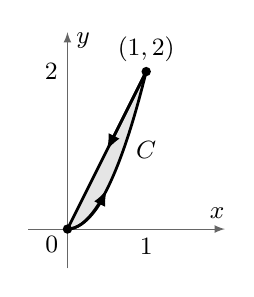
\begin{tikzpicture}
   \usetikzlibrary{arrows}
   \fill [fill=black!10] (0,0) parabola (1,2) -- (0,0);
   \draw [black!60,line width=0.3pt,-latex] (-0.5,0) -- (2,0);
   \draw [black!60,line width=0.3pt,-latex] (0,-0.5) -- (0,2.5);
   \pgfputat{\pgfpointxyz{1.9}{0.2}{0}}{\pgfbox[center,center]{\small $x$}}
   \pgfputat{\pgfpointxyz{0.2}{2.4}{0}}{\pgfbox[center,center]{\small $y$}}
   \pgfputat{\pgfpointxyz{-0.2}{-0.2}{0}}{\pgfbox[center,center]{\small $0$}}
   \draw [line width=1pt] (0,0) parabola (1,2);
   \draw [line width=1pt,-latex] (0,0) parabola (0.5,0.5);
   \draw [line width=1pt] (0,0) -- (1,2);
   \draw [line width=1pt,-latex] (1,2) -- (0.5,1);
   \node [right,above] at (1,2) {\small $(1,2)$};
   \node [left] at (0,2) {\small $2$};
   \node [below] at (1,0) {\small $1$};
   \node at (1,1) {\small $C$};
   \fill (0,0) circle (1.7pt);
   \fill (1,2) circle (1.7pt);
  \end{tikzpicture}}
 \par\noindent \emph{Solution:} $R$ is the shaded region in Figure 4.3.2. By Green's Theorem, for
 $P(x,y)=x^2 + y^2$ and $Q(x,y)=2xy$, we have
 \begin{align*}
  \oint_C (x^2 + y^2 )\,dx + 2xy\,dy ~&=~ \iint\limits_{R} \left( \frac{\partial Q}{\partial x} -
   \frac{\partial P}{\partial y} \right)\,dA\\
   &=~ \iint\limits_{R} (2y - 2y)\,dA
   ~=~ \iint\limits_{R} 0\,dA ~=~ 0 ~.
 \end{align*}
 \picskip{0}
 We actually already knew that the answer was zero. Recall from Example
 \ref{exmp:lineintexmpclosed} in Section 4.2 that the vector field
 $\mathbf{f}(x,y) = ( x^2 + y^2 )\,\mathbf{i} + 2xy\,\mathbf{j}$ has a potential function
 $F(x,y)=\frac{1}{3}x^3 + xy^2$, and so $\olineintvec{C}{f}{r} = 0$ by Corollary \ref{cor:lineintsuffpath}.
 \end{exmp}
\hrule width \textwidth height 0.5pt
\begin{exmp}\label{exmp:greenhole}
 Let $\mathbf{f}(x,y) = P(x,y)\,\mathbf{i} + Q(x,y)\,\mathbf{j}$, where
 \begin{displaymath}
  P(x,y) = \frac{-y}{x^2 + y^2} \quad\text{and}\quad Q(x,y) = \frac{x}{x^2 + y^2} ~,
 \end{displaymath}
 and let $R =\lbrace\,(x,y): 0 < x^2 + y^2 \le 1\,\rbrace$. For the boundary curve $C:x^2 + y^2 = 1$, traversed
 counterclockwise, it was shown in Exercise 9(b) in Section 4.2 that $\olineintvec{C}{f}{r} = 2\pi$. But
 \begin{displaymath}
  \frac{\partial Q}{\partial x} ~=~ \frac{y^2 - x^2}{(x^2 + y^2 )^2} ~=~ \frac{\partial P}{\partial y} ~
  \Rightarrow ~
  \iint\limits_{R} \left( \frac{\partial Q}{\partial x} - \frac{\partial P}{\partial y} \right)\,dA ~=~
  \iint\limits_{R} 0 \,dA = 0~.
 \end{displaymath}
\end{exmp}
This would seem to contradict Green's Theorem. However, note that $R$ is not the \emph{entire} region enclosed by $C$,
since the point $(0,0)$ is not contained in $R$. That is, $R$ has a ``hole'' at the origin, so Green's Theorem does not
apply.

\piccaption[]{\quad The annulus $R$}\parpic[r]{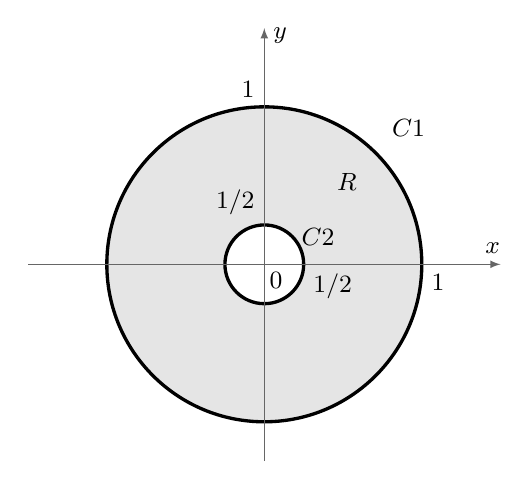
\begin{tikzpicture}
 \usetikzlibrary{arrows}
 \filldraw [black,line width=1.2pt,fill=black!10] (0:0) circle (2);
 \filldraw [black,line width=1.2pt,fill=white] (0:0) circle (0.5);
 \draw [black!60,line width=0.3pt,-latex] (-3,0) -- (3,0,0);
 \draw [black!60,line width=0.3pt,-latex] (0,-2.5) -- (0,3,0);
 \pgfputat{\pgfpointxyz{2.9}{0.2}{0}}{\pgfbox[center,center]{\small $x$}};
 \pgfputat{\pgfpointxyz{0.2}{2.9}{0}}{\pgfbox[center,center]{\small $y$}};
 \pgfputat{\pgfpointxyz{0.15}{-0.2}{0}}{\pgfbox[center,center]{\small $0$}};
 \node [above right] at (1.5,1.5) {\small $\ssub{C}{1}$};
 \node [right] at (0.35,0.35) {\small $\ssub{C}{2}$};
 \node [above left] at (0,2) {\small $1$};
 \node [below right] at (2,0) {\small $1$};
 \node [above left] at (0,0.5) {\small $1/2$};
 \node [below right] at (0.5,0) {\small $1/2$};
 \node at (1.05,1.05) {\small $R$};
 \node [rotate=45] at (-0.3536,0.3536) {\Large $\blacktriangleright$};
 \node [rotate=-45] at (1.4142,1.4142) {\Large $\blacktriangleleft$};
\end{tikzpicture}}
If we modify the region $R$ to be the \emph{annulus} $R =\lbrace\,(x,y): 1/4 \le x^2 + y^2 \le 1\,\rbrace$ (see
Figure 4.3.3), and take the ``boundary'' $C$ of $R$ to be $C = \ssub{C}{1} \cup \ssub{C}{2}$,
where $\ssub{C}{1}$ is\index{annulus}
the unit circle $x^2 + y^2 = 1$ traversed counterclockwise and $\ssub{C}{2}$ is the circle $x^2 + y^2 = 1/4$
traversed \emph{clockwise}, then it can be shown (see Exercise 8) that
\begin{displaymath}
 \olineintvec{C}{f}{r} ~=~ 0 ~.
\end{displaymath}
We would still have $\iint\limits_{R} \left( \frac{\partial Q}{\partial x} - \frac{\partial P}{\partial y} \right)\,dA
= 0$, so for this $R$ we would have
\begin{displaymath}
 \olineintvec{C}{f}{r} ~=~
 \iint\limits_{R} \left( \frac{\partial Q}{\partial x} - \frac{\partial P}{\partial y} \right)\,dA ~,
\end{displaymath}
which shows that Green's Theorem holds for the annular region $R$.\medskip
\hrule width \textwidth height 0.5pt
\medskip

It turns out that Green's Theorem can be extended to \emph{multiply connected} regions, that is, regions like
the annulus in Example \ref{exmp:greenhole}, which have one or more \emph{regions} cut out from the interior, as
opposed to discrete \emph{points} being cut out. For such
regions, the ``outer'' boundary and the ``inner'' boundaries are traversed so that $R$ is always on the left
side.\index{multiply connected}

\begin{figure}[h]
 \centering
 \subfloat[][Region $R$ with one hole]{
 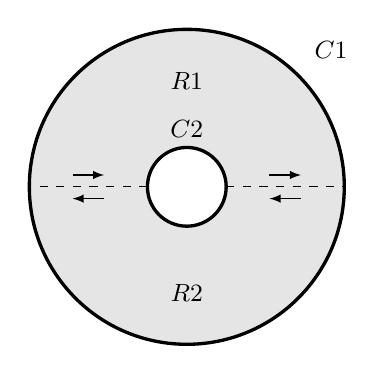
\begin{tikzpicture}
  \usetikzlibrary{arrows}
  \filldraw [black,line width=1.2pt,fill=black!10] (0:0) circle (2);
  \filldraw [black,line width=1.2pt,fill=white] (0:0) circle (0.5);
  \node [above right] at (1.5,1.5) {\small $\ssub{C}{1}$};
  \node [above] at (0,0.5) {\small $\ssub{C}{2}$};
  \node at (0,1.35) {\small $\ssub{R}{1}$};
  \node at (0,-1.35) {\small $\ssub{R}{2}$};
  \node [rotate=45] at (-0.3536,0.3536) {\Large $\blacktriangleright$};
  \node [rotate=45] at (0.3536,-0.3536) {\Large $\blacktriangleleft$};
  \node [rotate=-45] at (1.4142,1.4142) {\Large $\blacktriangleleft$};
  \node [rotate=-45] at (-1.4142,-1.4142) {\Large $\blacktriangleright$};
  \draw [dashed] (0.5,0) -- (2,0);
  \draw [dashed] (-0.5,0) -- (-2,0);
  \draw [-latex] (1.05,0.15) -- (1.45,0.15);
  \draw [latex-] (1.05,-0.15) -- (1.45,-0.15);
  \draw [-latex] (-1.45,0.15) -- (-1.05,0.15);
  \draw [latex-] (-1.45,-0.15) -- (-1.05,-0.15);
 \end{tikzpicture}}
 \qquad\qquad
 \subfloat[][Region $R$ with two holes]{
 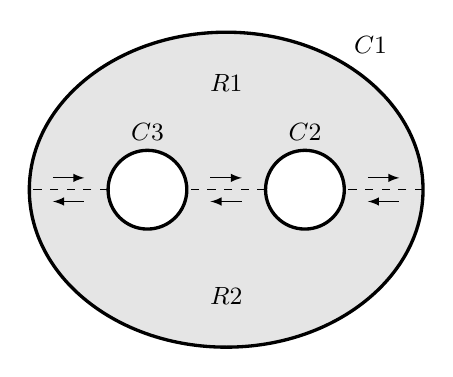
\begin{tikzpicture}
  \usetikzlibrary{arrows}
  \filldraw [black,line width=1.2pt,fill=black!10] (0,0) ellipse (2.5 and 2);
  \filldraw [black,line width=1.2pt,fill=white] (-1,0) circle (0.5);
  \filldraw [black,line width=1.2pt,fill=white] (1,0) circle (0.5);
  \node [above right] at (1.5,1.6) {\small $\ssub{C}{1}$};
  \node [above] at (1,0.5) {\small $\ssub{C}{2}$};
  \node [above] at (-1,0.5) {\small $\ssub{C}{3}$};
  \node at (0,1.35) {\small $\ssub{R}{1}$};
  \node at (0,-1.35) {\small $\ssub{R}{2}$};
  \node [rotate=45] at (-1.3536,0.3536) {\Large $\blacktriangleright$};
  \node [rotate=45] at (0.6464,0.3536) {\Large $\blacktriangleright$};
  \node [rotate=45] at (-0.6464,-0.3536) {\Large $\blacktriangleleft$};
  \node [rotate=45] at (1.3536,-0.3536) {\Large $\blacktriangleleft$};
  \node [rotate=-31] at (1.5,1.6) {\Large $\blacktriangleleft$};
  \node [rotate=-31] at (-1.5,-1.6) {\Large $\blacktriangleright$};
  \draw [dashed] (2.5,0) -- (1.5,0);
  \draw [dashed] (0.5,0) -- (-0.5,0);
  \draw [dashed] (-1.5,0) -- (-2.5,0);
  \draw [-latex] (1.8,0.15) -- (2.2,0.15);
  \draw [latex-] (1.8,-0.15) -- (2.2,-0.15);
  \draw [-latex] (-0.2,0.15) -- (0.2,0.15);
  \draw [latex-] (-0.2,-0.15) -- (0.2,-0.15);
  \draw [-latex] (-2.2,0.15) -- (-1.8,0.15);
  \draw [latex-] (-2.2,-0.15) -- (-1.8,-0.15);
 \end{tikzpicture}}
 \caption[]{\quad Multiply connected regions}
 \label{fig:multconn}
\end{figure}

The intuitive idea for why Green's Theorem holds for multiply connected regions is shown in Figure \ref{fig:multconn}
above. The idea is to cut ``slits'' between the boundaries of a multiply connected region $R$ so that $R$ is divided
into subregions which do \emph{not} have any ``holes''. For example, in Figure \ref{fig:multconn}(a) the region $R$
is the union of the regions $\ssub{R}{1}$ and $\ssub{R}{2}$, which are divided by the slits indicated by the dashed
lines. Those slits are part of the boundary of both $\ssub{R}{1}$ and $\ssub{R}{2}$, and we traverse then in the manner
indicated by the arrows. Notice that along each slit
the boundary of $\ssub{R}{1}$ is traversed in the opposite direction as that of $\ssub{R}{2}$, which means that the
line integrals of $\mathbf{f}$ along those slits cancel each other out.
Since $\ssub{R}{1}$ and $\ssub{R}{2}$ do not have holes in them, then Green's Theorem holds in each subregion, so that
\begin{displaymath}
 \olineintvec{\substack{\text{bdy}\\\text{of}~\ssub{R}{1}}}{f}{r} ~=~ \iint\limits_{\ssub{R}{1}}
  \left( \frac{\partial Q}{\partial x} - \frac{\partial P}{\partial y} \right)\,dA \quad\text{and}\quad
 \olineintvec{\substack{\text{bdy}\\\text{of}~\ssub{R}{2}}}{f}{r} ~=~ \iint\limits_{\ssub{R}{2}}
  \left( \frac{\partial Q}{\partial x} - \frac{\partial P}{\partial y} \right)\,dA ~.
\end{displaymath}
But since the line integrals along the slits cancel out, we have
\begin{displaymath}
 \olineintvec{\ssub{C}{1} \cup \ssub{C}{2}}{f}{r} ~=~
 \olineintvec{\substack{\text{bdy}\\\text{of}~\ssub{R}{1}}}{f}{r} ~+~
 \olineintvec{\substack{\text{bdy}\\\text{of}~\ssub{R}{2}}}{f}{r} ~,
\end{displaymath}
and so
\begin{displaymath}
 \olineintvec{\ssub{C}{1} \cup \ssub{C}{2}}{f}{r} ~=~ \iint\limits_{\ssub{R}{1}}
  \left( \frac{\partial Q}{\partial x} - \frac{\partial P}{\partial y} \right)\,dA ~+~ \iint\limits_{\ssub{R}{2}}
  \left( \frac{\partial Q}{\partial x} - \frac{\partial P}{\partial y} \right)\,dA ~=~ \iint\limits_{R}
  \left( \frac{\partial Q}{\partial x} - \frac{\partial P}{\partial y} \right)\,dA ~,
\end{displaymath}
which shows that Green's Theorem holds in the region $R$. A similar argument shows that the theorem holds in the
region with two holes shown in Figure \ref{fig:multconn}(b).

We know from Corollary \ref{cor:lineintsuffpath} that when a smooth vector field
$\mathbf{f}(x,y) = P(x,y)\,\mathbf{i} + Q(x,y)\,\mathbf{j}$ on a region $R$ (whose boundary is a piecewise smooth,
simple closed curve $C$) has a potential in $R$, then $\olineintvec{C}{f}{r} = 0$. And if the potential
$F(x,y)$ is smooth in $R$, then
$\frac{\partial F}{\partial x} = P$ and $\frac{\partial F}{\partial y} = Q$, and so we know that
\begin{displaymath}
 \frac{\partial^2 F}{\partial y \,\partial x} = \frac{\partial^2 F}{\partial x \,\partial y} ~\Rightarrow~
 \frac{\partial P}{\partial y} = \frac{\partial Q}{\partial x} ~~\text{in $R$.}
\end{displaymath}
Conversely, if $\frac{\partial P}{\partial y} = \frac{\partial Q}{\partial x}$ in $R$ then
\begin{displaymath}
 \olineintvec{C}{f}{r} ~=~ \iint\limits_{R} \left( \frac{\partial Q}{\partial x} -
   \frac{\partial P}{\partial y} \right)\,dA ~=~ \iint\limits_{R} 0\,dA ~=~ 0 ~.
\end{displaymath}
For a \textbf{simply connected}\index{simply connected} region $R$ (i.e. a region with no holes), the following can be
shown:\index{path independence}\medskip
\statecomment{
 {The following statements are equivalent for a simply connected region $R$ in $\Real{2}$:
  \begin{enumerate}[(a)]
  \item $\mathbf{f}(x,y) ~=~ P(x,y)\,\mathbf{i} + Q(x,y)\,\mathbf{j}$ has a smooth potential $F(x,y)$ in $R$
  \item $\displaystyle{\lineintvec{C}{f}{r}}$ is independent of the path for any curve $C$ in $R$
  \item $\displaystyle{\olineintvec{C}{f}{r}} ~=~ 0$ for every simple closed curve $C$ in $R$
  \item $\dfrac{\partial P}{\partial y} = \dfrac{\partial Q}{\partial x}$ in $R$\quad
   (in this case, the differential form $P\,dx + Q\,dy$ is exact)\index{exact differential form}
 \end{enumerate}}}
%\startexercises
\centerline{\fbox{\textsf{\textbf{\large Exercises}}}}
\label{sec4dot3}
\probs{A}
\par\noindent For Exercises 1--4, use Green's Theorem to evaluate the given line integral around the curve $C$, traversed
counterclockwise.
\begin{enumerate}[\bfseries 1.]
 \item $\displaystyle\oint_C (x^2 - y^2 )\,dx + 2xy\,dy$; $C$ is the boundary
  of $R = \lbrace\,(x,y): 0 \le x \le 1,~2x^2 \le y \le 2x \,\rbrace$
 \item $\displaystyle\oint_C x^2 y\,dx + 2xy\,dy$; $C$ is the boundary
  of $R = \lbrace\,(x,y): 0 \le x \le 1,~x^2 \le y \le x \,\rbrace$
 \item $\displaystyle\oint_C 2y\,dx - 3x\,dy$; $C$ is the circle $x^2 + y^2 = 1$
 \item $\displaystyle\oint_C (e^{x^2} + y^2 )\,dx + (e^{y^2} + x^2 )\,dy$; $C$ is the boundary of the triangle with
  vertices $(0,0)$, $(4,0)$ and $(0,4)$
 \item Is there a potential $F(x,y)$ for $\mathbf{f}(x,y) = (y^2 + 3x^2 )\,\mathbf{i} + 2xy\,\mathbf{j}$?
  If so, find one.
 \item Is there a potential $F(x,y)$ for $\mathbf{f}(x,y) = (x^3 \cos (xy) + 2x \sin (xy))\,\mathbf{i} +
  x^2 y \cos (xy)\,\mathbf{j}$? If so, find one.
 \item Is there a potential $F(x,y)$ for $\mathbf{f}(x,y) = (8xy+3)\,\mathbf{i} +
  4(x^2 + y)\,\mathbf{j}$? If so, find one.
 \item Show that 
 \[\displaystyle\oint_C a\,dx + b\,dy = 0\]
 for any constants $a$, $b$ and any closed simple curve $C$.
\suspend{enumerate}
\probs{B}
\resume{enumerate}[{[\bfseries 1.]}]
 \item For the vector field $\mathbf{f}$ as in Example \ref{exmp:greenhole}, show directly that
 $\olineintvec{C}{f}{r} = 0$, where
 $C$ is the boundary of the annulus $R =\lbrace\,(x,y): 1/4 \le x^2 + y^2 \le 1\,\rbrace$ traversed so that $R$ is
 always on the left.
 \item Evaluate \[\oint_C  e^x \,\sin y\,dx + (y^3 + e^x \,\cos y)\,dy,\] where $C$ is the boundary of the
  rectangle with vertices $(1,-1)$, $(1,1)$, $(-1,1)$ and $(-1,-1)$, traversed counterclockwise.
\suspend{enumerate}
\probs{C}
\resume{enumerate}[{[\bfseries 1.]}]
 \item\label{ex:green-area} For a region $R$ bounded by a simple closed curve $C$, show that the area $A$ of $R$ is
  \begin{displaymath}
   A ~=~ -\oint_C y\,dx ~=~ \oint_C x\,dy ~=~ \frac{1}{2}\oint_C x\,dy - y\,dx ~,
  \end{displaymath}
  where $C$ is traversed so that $R$ is always on the left.
  (\emph{Hint: Use Green's Theorem and the fact that $A = \iint_{R} 1\,dA$}.)
\suspend{enumerate}
Use Exercise~\ref{ex:green-area} to find the area bounded by curve.
\resume{enumerate}[{[\bfseries 1.]}]

\item The curve $(\sin t,\sin(2 t))$ for $0\le t\le \pi$ 


\item The deltoid curve $(2\cos t+\cos 2t,2\sin t-\sin 2t)$ for $0\le t\le 2\pi$. 
(The deltoid curve is shown on the diagram; you can assume without proof that it has no self-intesections.)
\end{enumerate}

\begin{center}
\begin{lpic}[t(-4 mm),b(0 mm),r(0 mm),l(0 mm)]{pics/deltoid(1)}
%\lbl[rt]{22.5,15.5;$P$}
\end{lpic}
\end{center}

\newpage
%Begin Section 4.4
\section{Surface Integrals and the Divergence Theorem}
In Section 4.1 we learned how to integrate along a curve. We will now learn how to perform integration over a
\emph{surface} in $\Real{3}$, such as a sphere or a paraboloid.\index{integral!surface}\index{surface integral}
Recall from Section 1.8 how we identified points $(x,y,z)$ on a curve $C$ in $\Real{3}$,
parametrized by $x=x(t)$, $y=y(t)$, $z=z(t)$, $a \le t \le b$, with the terminal points of the position vector
\begin{displaymath}
 \mathbf{r}(t) = x(t) \mathbf{i} + y(t) \mathbf{j} + z(t) \mathbf{k} ~~\text{for $t$ in $\ival{a}{b}$.}
\end{displaymath}

The idea behind a parametrization of a curve is that it ``transforms'' a subset of $\Real{1}$ (normally an interval
$\ival{a}{b}$) into a curve in $\Real{2}$ or $\Real{3}$ (see Figure \ref{fig:curveparam}).

\begin{figure}[h]
 \begin{center}
  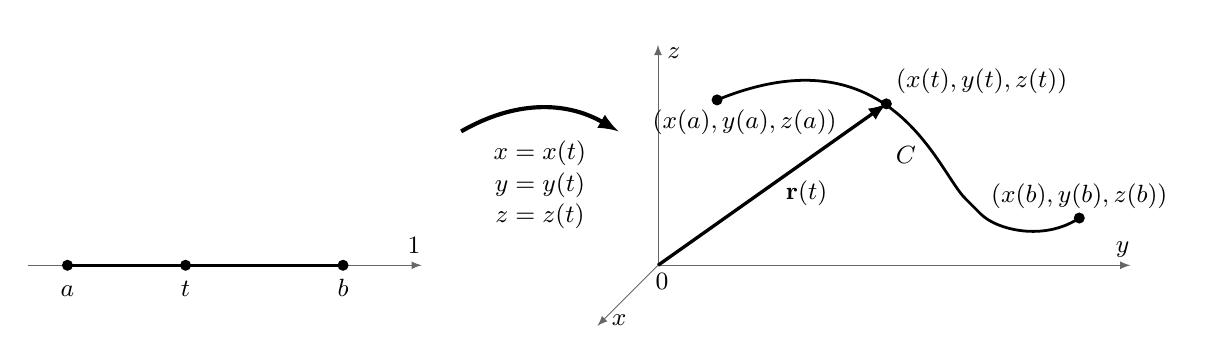
\begin{tikzpicture}
   \usetikzlibrary{arrows}
   \draw [black!60,line width=0.3pt,-latex,anchor=base] (-2,0) -- (3,0,0)
    node[black,shift={(0,-0.4)}] at (-1.5,0) {\small $a$}
    node[black,shift={(0,-0.4)}] at (0,0) {\small $t$}
    node[black,shift={(0,-0.4)}] at (2,0) {\small $b$};
   \pgfputat{\pgfpointxyz{2.9}{0.25}{0}}{\pgfbox[center,center]{\small $\Real{1}$}};
   \draw [line width=1.2pt] (-1.5,0) -- (2,0);
   \fill (-1.5,0) circle (2pt);
   \fill (0,0) circle (2pt);
   \fill (2,0) circle (2pt);
   \draw [black!60,line width=0.3pt,-latex] (6,0) -- (12,0,0);
   \draw [black!60,line width=0.3pt,-latex] (6,0) -- (6,2.8,0);
   \draw [black!60,line width=0.3pt,-latex] (6,0) -- (6,0,2);
   \pgfputat{\pgfpointxyz{11.9}{0.2}{0}}{\pgfbox[center,center]{\small $y$}};
   \pgfputat{\pgfpointxyz{6.2}{2.7}{0}}{\pgfbox[center,center]{\small $z$}};
   \pgfputat{\pgfpointxyz{6.2}{0}{1.8}}{\pgfbox[center,center]{\small $x$}};
   \pgfputat{\pgfpointxyz{6.05}{-0.2}{0}}{\pgfbox[center,center]{\small $0$}};
   \draw [rounded corners,line width=1pt](6.75,2.1) .. controls (8.95,3) and (9.55,1.2) .. (10,0.75) ..
    controls (10.3,0.45) and (10.9,0.3) .. (11.35,0.6);
   \draw [black,line width=1.2pt,-latex] (6,0) -- (8.9,2.05);
   \node [below] at (7.1,2.1) {\small $(x(a),y(a),z(a))$};
   \node [above right] at (8.9,2.05) {\small $(x(t),y(t),z(t))$};
   \node [above] at (11.35,0.6) {\small $(x(b),y(b),z(b))$};
   \node [below right] at (7.5,1.2) {\small $\mathbf{r}(t)$};
   \node [left] at (9.4,1.4) {\small $C$};
   \fill (6.75,2.1) circle (2pt);
   \fill (8.9,2.05) circle (2pt);
   \fill (11.35,0.6) circle (2pt);
   \draw [line width=1.5pt,-latex]  (3.5,1.7) to[out=30,in=150] (5.5,1.7);
   \node [below] at (4.5,1.7) {\small $x=x(t)$};
   \node [below] at (4.5,1.3) {\small $y=y(t)$};
   \node [below] at (4.5,0.9) {\small $z=z(t)$};
  \end{tikzpicture}
 \end{center}
 \caption[]{\quad Parametrization of a curve $C$ in $\Real{3}$}
 \label{fig:curveparam}
\end{figure}

Similar to how we used a parametrization of a curve to define the line integral along the curve, we will use a
parametrization of a surface to define a \emph{surface integral}. We will use \emph{two} variables, $u$ and $v$,
to parametrize a surface $\Sigma$ in $\Real{3}$: $x=x(u,v)$, $y=y(u,v)$, $z=z(u,v)$, for $(u,v)$ in some region $R$ in
$\Real{2}$ (see Figure \ref{fig:surfparam}).

\begin{figure}[h]
 \begin{center}
  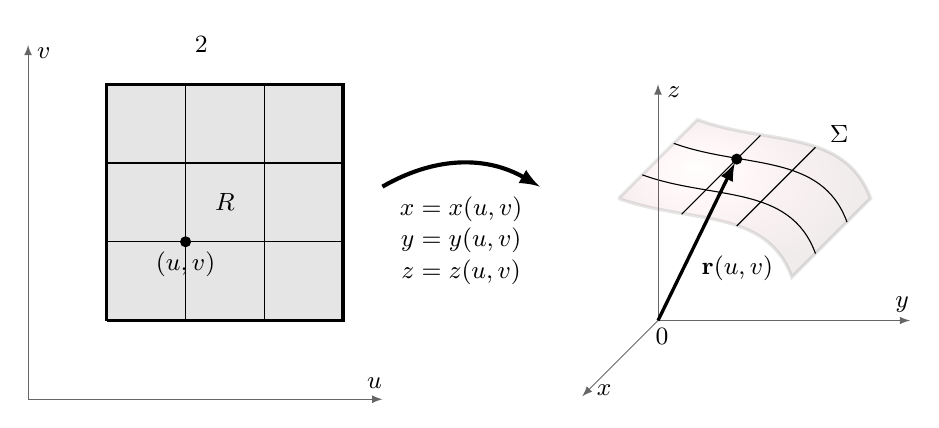
\begin{tikzpicture}
   \usetikzlibrary{arrows}
   \draw [black!60,line width=0.3pt,-latex] (0,0) -- (4.5,0);
   \draw [black!60,line width=0.3pt,-latex] (0,0) -- (0,4.5);
   \pgfputat{\pgfpointxyz{4.4}{0.2}{0}}{\pgfbox[center,center]{\small $u$}}
   \pgfputat{\pgfpointxyz{0.2}{4.4}{0}}{\pgfbox[center,center]{\small $v$}}
   \filldraw [black,line width=1.2pt,fill=black!10] (1,1) -- (1,4) -- (4,4) -- (4,1) -- (1,1);
   \draw (1,2) -- (4,2);
   \draw (1,3) -- (4,3);
   \draw (2,1) -- (2,4);
   \draw (3,1) -- (3,4);
   \node at (2.5,2.5) {\small $R$};
   \node at (2.2,4.5) {\small $\Real{2}$};
   \node [below] at (2,2) {\small $(u,v)$};
   \fill (2,2) circle (2pt);
   \shadedraw [line width=1.2pt,opacity=0.1,ball color=red!40] (7.5,2.55) to[out=-20,in=110] (9.7,1.55) -- (10.7,2.55)
    to[out=110,in=-20] (8.5,3.55) -- (7.5,2.55);
   \draw (7.8,2.85) to[out=-20,in=110] (10,1.85);
   \draw (8.2,3.25) to[out=-20,in=110] (10.4,2.25);
   \draw (9.3,3.35) -- (8.3,2.35);
   \draw (10,3.2) -- (9,2.2);
   \draw [black!60,line width=0.3pt,-latex] (8,1) -- (11.2,1,0);
   \draw [black!60,line width=0.3pt,-latex] (8,1) -- (8,4,0);
   \draw [black!60,line width=0.3pt,-latex] (8,1) -- (8,1,2.5);
   \pgfputat{\pgfpointxyz{11.1}{1.2}{0}}{\pgfbox[center,center]{\small $y$}};
   \pgfputat{\pgfpointxyz{8.2}{3.9}{0}}{\pgfbox[center,center]{\small $z$}};
   \pgfputat{\pgfpointxyz{8.2}{1}{2.3}}{\pgfbox[center,center]{\small $x$}};
   \pgfputat{\pgfpointxyz{8.05}{0.8}{0}}{\pgfbox[center,center]{\small $0$}};
   \node [below] at (10.3,3.6) {\small $\Sigma$};
   \fill (9,3.05) circle (2pt);
   \draw [black,line width=1.2pt,-latex] (8,1) -- (8.975,3);
   \node [below right] at (8.43,1.95) {\small $\mathbf{r}(u,v)$};
   \draw [line width=1.5pt,-latex]  (4.5,2.7) to[out=30,in=150] (6.5,2.7);
   \node [below] at (5.5,2.7) {\small $x=x(u,v)$};
   \node [below] at (5.5,2.3) {\small $y=y(u,v)$};
   \node [below] at (5.5,1.9) {\small $z=z(u,v)$};
  \end{tikzpicture}
 \end{center}
 \caption[]{\quad Parametrization of a surface $\Sigma$ in $\Real{3}$}
 \label{fig:surfparam}
\end{figure}

In this case, the position vector of a point on the surface $\Sigma$ is given by the vector-valued function
\begin{displaymath}
 \mathbf{r}(u,v) ~=~ x(u,v) \mathbf{i} ~+~ y(u,v) \mathbf{j} ~+~ z(u,v) \mathbf{k} ~~\text{for $(u,v)$ in $R$.}
\end{displaymath}

Since $\mathbf{r}(u,v)$ is a function of two variables, define the partial derivatives
$\frac{\partial \mathbf{r}}{\partial u}$ and $\frac{\partial \mathbf{r}}{\partial v}$ for $(u,v)$ in $R$ by
\begin{align*}
 \frac{\partial \mathbf{r}}{\partial u}(u,v) ~&=~
 \frac{\partial x}{\partial u}(u,v) \mathbf{i} ~+~ \frac{\partial y}{\partial u}(u,v) \mathbf{j} ~+~
 \frac{\partial z}{\partial u}(u,v) \mathbf{k} ~,~~\text{and}\smallskip\\
 \frac{\partial \mathbf{r}}{\partial v}(u,v) ~&=~
 \frac{\partial x}{\partial v}(u,v) \mathbf{i} ~+~ \frac{\partial y}{\partial v}(u,v) \mathbf{j} ~+~
 \frac{\partial z}{\partial v}(u,v) \mathbf{k} ~.
\end{align*}

The parametrization of $\Sigma$ can be thought of as ``transforming'' a region in $\Real{2}$ (in the $uv$-plane) into
a 2-dimensional surface in $\Real{3}$. This parametrization of the surface is sometimes called a \emph{patch}, based
on the idea of ``patching'' the region $R$ onto $\Sigma$ in the grid-like manner shown in Figure \ref{fig:surfparam}.

In fact, those gridlines in $R$ lead us to how we will define a surface integral over $\Sigma$. Along the
vertical gridlines in $R$, the variable $u$ is constant. So those lines get mapped to curves on $\Sigma$, and the
variable $u$ is constant along the position vector $\mathbf{r}(u,v)$. Thus, the tangent vector to those curves at a
point $(u,v)$ is $\frac{\partial \mathbf{r}}{\partial v}$. Similarly, the horizontal gridlines in $R$ get mapped to
curves on $\Sigma$ whose tangent vectors are $\frac{\partial \mathbf{r}}{\partial u}$.

Now take a point $(u,v)$ in $R$ as, say,
the lower left corner of one of the rectangular grid sections in $R$, as shown in Figure \ref{fig:surfparam}. Suppose
that this rectangle has a small width and height of $\Delta u$ and $\Delta v$, respectively. The corner points of that
rectangle are $(u,v)$, $(u+\Delta u,v)$, $(u+\Delta u,v+\Delta v)$ and $(u,v+\Delta v)$.
So the area of that
rectangle is $A = \Delta u\,\Delta v$. Then that rectangle gets mapped by the parametrization onto some section of the
surface $\Sigma$ which, for $\Delta u$ and $\Delta v$ small enough, will have a surface area (call it $d\sigma$) that
is very close to the area of the parallelogram which has adjacent sides $\mathbf{r}(u+\Delta u,v) - \mathbf{r}(u,v)$
(corresponding to the line segment from $(u,v)$ to $(u+\Delta u,v)$ in $R$) and
$\mathbf{r}(u,v+\Delta v) - \mathbf{r}(u,v)$ (corresponding to the line segment from $(u,v)$ to $(u,v+\Delta v)$ in
$R$). But by combining our usual notion of a partial derivative (see Definition \ref{defn:partial} in
Section 2.2) with that of the derivative of a vector-valued function (see Definition \ref{defn:veccont} in
Section 1.8) applied to a function of two variables, we have
\begin{align*}
 \frac{\partial \mathbf{r}}{\partial u} ~&\approx~ \frac{\mathbf{r}(u+\Delta u,v) - \mathbf{r}(u,v)}{\Delta u}
 ~,~~\text{and}\smallskip\\
 \frac{\partial \mathbf{r}}{\partial v} ~&\approx~ \frac{\mathbf{r}(u,v+\Delta v) - \mathbf{r}(u,v)}{\Delta v} ~,
\end{align*}
and so the surface area element $d\sigma$ is approximately
\begin{displaymath}
 \Norm{\Crossprod{(\mathbf{r}(u+\Delta u,v) - \mathbf{r}(u,v))}{(\mathbf{r}(u,v+\Delta v) - \mathbf{r}(u,v))}} \approx
 \NORM{\Crossprod{(\Delta u \frac{\partial \mathbf{r}}{\partial u})}{(\Delta v\frac{\partial \mathbf{r}}{\partial v})}}
 = \NORM{\Crossprod{\frac{\partial \mathbf{r}}{\partial u}}{\frac{\partial \mathbf{r}}{\partial v}}}\,
 \Delta u \, \Delta v
\end{displaymath}
by Theorem \ref{thm:crossarea} in Section 1.4.
Thus, the total surface area $S$ of $\Sigma$ is approximately the sum of all the quantities
$\Norm{\Crossprod{\frac{\partial \mathbf{r}}{\partial u}}{\frac{\partial \mathbf{r}}{\partial v}}}\,\Delta u\,\Delta v$,
summed over the rectangles in $R$. Taking the limit of that sum as the diagonal of the largest rectangle goes to $0$
gives
\begin{equation}
 S ~=~ \iint\limits_{R}\,\NORM{\Crossprod{\frac{\partial \mathbf{r}}{\partial u}}{\frac{\partial \mathbf{r}}{\partial v}}}
 \,du\,dv ~.
\end{equation}
We will write the double integral on the right using the special notation
\begin{equation}
 \iint\limits_{\Sigma} d\sigma ~=~
 \iint\limits_{R}\,\NORM{\Crossprod{\frac{\partial \mathbf{r}}{\partial u}}{\frac{\partial \mathbf{r}}{\partial v}}}
 \,du\,dv ~.
\end{equation}
This is a special case of a \emph{surface integral} over the surface $\Sigma$, where the surface area element
$d\sigma$ can be thought of as $1\,d\sigma$. Replacing $1$ by a general real-valued function $f(x,y,z)$ defined
in $\Real{3}$, we have the following:

\statedefn{defn:surfintreal}{
 {Let $\Sigma$ be a surface in $\Real{3}$ parametrized by $x=x(u,v)$, $y=y(u,v)$,\\$z=z(u,v)$, for $(u,v)$ in some
  region $R$ in $\Real{2}$. 
  Let $\mathbf{r}(u,v) = x(u,v) \mathbf{i} + y(u,v) \mathbf{j} + z(u,v) \mathbf{k}$ be the
  position vector for any point on $\Sigma$, and let $f(x,y,z)$ be a real-valued function defined on some subset
  of $\Real{3}$ that contains $\Sigma$. The \textbf{surface integral} of $f(x,y,z)$ over $\Sigma$ is
  \begin{equation}\label{eqn:surfintreal}
   \iint\limits_{\Sigma} f(x,y,z)\,d\sigma ~=~ \iint\limits_{R} f(x(u,v),y(u,v),z(u,v))\,
   \NORM{\Crossprod{\frac{\partial \mathbf{r}}{\partial u}}{\frac{\partial \mathbf{r}}{\partial v}}}\,du\,dv ~.
  \end{equation}
  In particular, the surface area $S$ of $\Sigma$ is\index{integral!surface}\index{surface integral}
  \begin{equation}
   S ~=~ \iint\limits_{\Sigma} 1\,d\sigma ~.
  \end{equation}}
}

\medskip
\hrule width \textwidth height 0.5pt
\begin{exmp}
 A \emph{torus} $T$ is a surface obtained by revolving a circle of radius $a$ in the $yz$-plane around the $z$-axis,
 where the circle's center is at a distance $b$ from the z-axis ($0<a<b$), as in Figure \ref{fig:torus}. Find the
 surface area of $T$.\index{torus}
 
 \begin{figure}[h]
 \centering
 \subfloat[][Circle in the $yz$-plane]{
 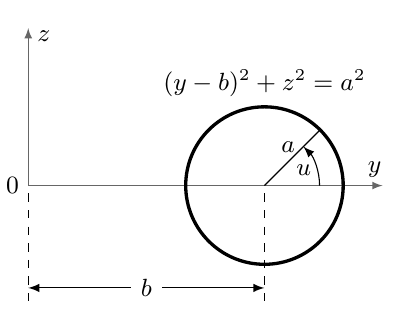
\begin{tikzpicture}
  \usetikzlibrary{arrows}
  \draw [black!60,line width=0.3pt,-latex] (0,0) -- (4.5,0);
  \draw [black!60,line width=0.3pt,-latex] (0,0) -- (0,2);
  \pgfputat{\pgfpointxyz{4.4}{0.2}{0}}{\pgfbox[center,center]{\small $y$}}
  \pgfputat{\pgfpointxyz{0.2}{1.9}{0}}{\pgfbox[center,center]{\small $z$}}
  \pgfputat{\pgfpointxyz{-0.2}{0}{0}}{\pgfbox[center,center]{\small $0$}}
  \draw [line width=1.2pt] (3,0) circle (1);
  \draw (3,0) -- (3.707,0.707);
  \draw [-latex] (3.7,0) arc (0:45:0.7);
  \node [above] at (3.3,0.3) {\small $a$};
  \node [above] at (3,1) {\small $(y-b)^2 + z^2 = a^2$};
  \node at (3.5,0.2) {\small $u$};
  \draw [dashed] (0,-0.1) -- (0,-1.5);
  \draw [dashed] (3,-0.1) -- (3,-1.5);
  \node at (1.5,-1.3) {\small $b$};
  \draw [-latex] (1.7,-1.3) -- (3,-1.3);
  \draw [-latex] (1.3,-1.3) -- (0,-1.3);
 \end{tikzpicture}}
 \qquad\qquad
 \subfloat[][Torus $T$]{\includegraphics{torus.0}}
 \caption[]{}
 \label{fig:torus}
\end{figure}

\par\noindent \emph{Solution:}
For any point on the circle, the line segment from the center of the circle to that point makes an angle $u$ with the
$y$-axis in the positive $y$ direction (see Figure \ref{fig:torus}(a)). And as the circle revolves around the $z$-axis,
the line segment from the origin to the center of that circle sweeps out an angle $v$ with the positive $x$-axis (see
Figure \ref{fig:torus}(b)). Thus, the torus can be parametrized as:
\begin{displaymath}
 x = (b+a\cos u)\cos v ~,\quad y = (b+a\cos u)\sin v ~,\quad z = a\sin u~,\quad 0\le u\le 2\pi~,\quad 0\le v\le 2\pi
\end{displaymath}
So for the position vector
\begin{align*}
 \mathbf{r}(u,v) ~&=~ x(u,v) \mathbf{i} ~+~ y(u,v) \mathbf{j} ~+~ z(u,v) \mathbf{k}\\
 &=~ (b+a\cos u)\cos v \,\mathbf{i} ~+~ (b+a\cos u)\sin v \,\mathbf{j} ~+~ a\sin u \,\mathbf{k}
\end{align*}
we see that
\begin{align*}
 \frac{\partial \mathbf{r}}{\partial u} ~&=~
  -a\sin u\,\cos v \,\mathbf{i} ~-~ a\sin u\,\sin v \,\mathbf{j} ~+~ a\cos u \,\mathbf{k}\\[6pt]
 \frac{\partial \mathbf{r}}{\partial v} ~&=~
  -(b+a\cos u)\sin v \,\mathbf{i} ~+~ (b+a\cos u)\cos v \,\mathbf{j} ~+~ 0 \mathbf{k} ~,
\end{align*}
and so computing the cross product gives
\begin{displaymath}
 \Crossprod{\frac{\partial \mathbf{r}}{\partial u}}{\frac{\partial \mathbf{r}}{\partial v}} ~=~
  -a(b+a\cos u)\cos v\,\cos u \,\mathbf{i} ~-~ a(b+a\cos u)\sin v\,\cos u\,\mathbf{j} ~-~ a(b+a\cos u)\sin u \,\mathbf{k} ~,
\end{displaymath}
which has magnitude
\begin{displaymath}
 \NORM{\Crossprod{\frac{\partial \mathbf{r}}{\partial u}}{\frac{\partial \mathbf{r}}{\partial v}}} ~=~ a(b+a\cos u) ~.
\end{displaymath}
Thus, the surface area of $T$ is
\begin{align*}
 S ~&=~ \iint\limits_{\Sigma} 1\,d\sigma\\[6pt]
  &=~ \int_0^{2\pi} \int_0^{2\pi}\,\NORM{\Crossprod{\frac{\partial \mathbf{r}}{\partial u}}{\frac{\partial
  \mathbf{r}}{\partial v}}}\,du\,dv\\[6pt]
  &=~ \int_0^{2\pi} \int_0^{2\pi} a(b+a\cos u)\,du\,dv\\[6pt]
  &=~ \int_0^{2\pi} \left( abu + a^2 \sin u \,\Big|_{u=0}^{u=2\pi}\,\right)\,dv\\[6pt]
  &=~ \int_0^{2\pi} 2\pi ab\,dv\\
  &=~ 4\pi^2 ab
\end{align*}
\end{exmp}
\hrule width \textwidth height 0.5pt
\medskip

Since $\frac{\partial \mathbf{r}}{\partial u}$ and $\frac{\partial \mathbf{r}}{\partial v}$ are tangent to the surface
$\Sigma$ (i.e. lie in the tangent plane to $\Sigma$ at each point on $\Sigma$), then their cross product
$\Crossprod{\frac{\partial \mathbf{r}}{\partial u}}{\frac{\partial \mathbf{r}}{\partial v}}$ is perpendicular to the
tangent plane to the surface at each point of $\Sigma$. Thus,

\begin{displaymath}
 \iint\limits_{\Sigma} f(x,y,z)\,d\sigma = \iint\limits_{R} f(x(u,v),y(u,v),z(u,v))\,\norm{\mathbf{n}}\,d\sigma ~,
\end{displaymath}
where $\mathbf{n} = \Crossprod{\frac{\partial \mathbf{r}}{\partial u}}{\frac{\partial \mathbf{r}}{\partial v}}$.
We say that $\mathbf{n}$ is a \textbf{normal vector} to $\Sigma$.\index{vector!normal}

\piccaption[]{}\parpic[r]{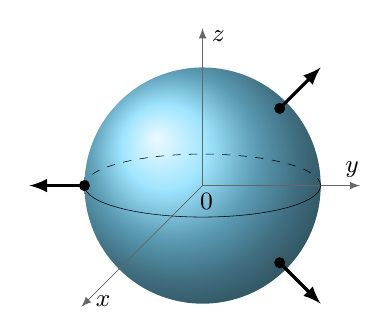
\begin{tikzpicture}
 \usetikzlibrary{arrows}
 \definecolor{spherecolor}{HTML}{80DCFF}
 \shade [ball color=spherecolor] (0,0) circle (1.5);
 \draw [black!60,line width=0.3pt,-latex] (0,0) -- (2,0,0);
 \draw [black!60,line width=0.3pt,-latex] (0,0) -- (0,2,0);
 \draw [black!60,line width=0.3pt,-latex] (0,0) -- (0,0,4);
 \pgfputat{\pgfpointxyz{1.9}{0.2}{0}}{\pgfbox[center,center]{\small $y$}};
 \pgfputat{\pgfpointxyz{0.2}{1.9}{0}}{\pgfbox[center,center]{\small $z$}};
 \pgfputat{\pgfpointxyz{0.2}{0}{3.8}}{\pgfbox[center,center]{\small $x$}};
 \pgfputat{\pgfpointxyz{0.05}{-0.2}{0}}{\pgfbox[center,center]{\small $0$}};
 \draw [line width=0.2pt] (-1.5,0) arc (180:360:1.5 and 0.4);
 \draw [dashed,line width=0.2pt] (1.5,0) arc (0:180:1.5 and 0.4);
 \fill (0.98,0.98) circle (2pt);
 \draw [line width=1.2pt,-latex] (0.98,0.98) -- (1.5,1.5);
 \fill (0.98,-0.98) circle (2pt);
 \draw [line width=1.2pt,-latex] (0.98,-0.98) -- (1.5,-1.5);
 \fill (-1.5,0) circle (2pt);
 \draw [line width=1.2pt,-latex] (-1.5,0) -- (-2.2,0);
\end{tikzpicture}}
Recall that normal vectors to a plane can point in two opposite directions. By an
\textbf{outward unit normal vector} to a surface $\Sigma$, we will mean the unit vector that is normal to $\Sigma$ and
points away from the ``top'' (or ``outer'' part) of the surface. This is a hazy definition, but the picture in
Figure 4.4.4 gives a better idea of what outward normal vectors look like, in the case of a sphere.
With this idea in mind, we make the following definition of a surface integral of a 3-dimensional
\emph{vector field} over a surface:\index{outward normal}

\statedefn{defn:surfintvec}{
 {Let $\Sigma$ be a surface in $\Real{3}$ and let $\mathbf{f}(x,y,z) = \ssub{f}{1}(x,y,z) \mathbf{i} +
  \ssub{f}{2}(x,y,z) \mathbf{j} + \ssub{f}{3}(x,y,z) \mathbf{k}$ be a vector field defined on some subset
  of $\Real{3}$ that contains $\Sigma$. The \textbf{surface integral} of $\mathbf{f}$ over $\Sigma$ is
  \begin{equation}\label{eqn:surfintvec}
   \iint\limits_{\Sigma} \Dotprod{\mathbf{f}}{d\bm{\sigma}} ~=~
   \iint\limits_{\Sigma} \Dotprod{\mathbf{f}}{\mathbf{n}}\,d\sigma ~,
  \end{equation}
  where, at any point on $\Sigma$, $\mathbf{n}$ is the outward unit normal vector to $\Sigma$.}
}

Note in the above definition that the dot product inside the integral on the right is a
real-valued function, and hence we can use Definition \ref{defn:surfintreal} to evaluate the integral.

\medskip
\hrule width \textwidth height 0.5pt
\begin{exmp}\label{exmp:surfintex}
 Evaluate the surface integral $\iint\limits_{\Sigma} \Dotprod{\mathbf{f}}{d\bm{\sigma}}$, where
 $\mathbf{f}(x,y,z) = yz\mathbf{i} + xz\mathbf{j} + xy\mathbf{k}$ and $\Sigma$ is the part of the plane $x+y+z=1$
 with $x \ge 0$, $y \ge 0$, and $z \ge 0$, with the outward unit normal $\mathbf{n}$ pointing in the positive $z$
 direction (see Figure 4.4.5).\smallskip
 \piccaption[]{}\parpic[r]{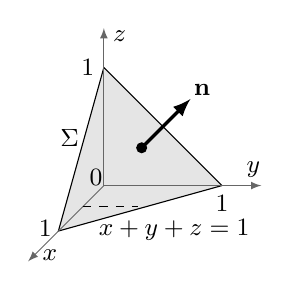
\begin{tikzpicture}
  \usetikzlibrary{arrows}
  \filldraw [black,fill=black!10] (1.5,0,0) -- (0,1.5,0) -- (0,0,1.5) -- (1.5,0,0);
  \draw [black!60,line width=0.3pt,-latex] (0,0) -- (2,0,0);
  \draw [black!60,line width=0.3pt,-latex] (0,0) -- (0,2,0);
  \draw [black!60,line width=0.3pt,-latex] (0,0) -- (0,0,2.5);
  \pgfputat{\pgfpointxyz{1.9}{0.2}{0}}{\pgfbox[center,center]{\small $y$}};
  \pgfputat{\pgfpointxyz{0.2}{1.9}{0}}{\pgfbox[center,center]{\small $z$}};
  \pgfputat{\pgfpointxyz{0.2}{0}{2.3}}{\pgfbox[center,center]{\small $x$}};
  \pgfputat{\pgfpointxyz{-0.1}{0.1}{0}}{\pgfbox[center,center]{\small $0$}};
  \node [below] at (1.5,0,0) {\small $1$};
  \node [left] at (0,1.5,0) {\small $1$};
  \node [left] at (0,0,1.4) {\small $1$};
  \node [left] at (0,0.8,0.5) {\small $\Sigma$};
  \node [below] at (1.2,0,0.8) {\small $x+y+z=1$};
  \draw [dashed] (0,0,0.7) -- (0.7,0,0.7);
  \fill (0.48,0.48) circle (2pt);
  \draw [line width=1.2pt,-latex] (0.48,0.48) -- (1.1,1.1);
  \node [above right] at (1.02,1.02) {\small $\mathbf{n}$};
 \end{tikzpicture}}
 \par\noindent \emph{Solution:} Since the vector $\mathbf{v} = (1,1,1)$ is normal to the plane $x+y+z=1$ (why?), then
 dividing $\mathbf{v}$ by its length yields the outward unit normal vector $\mathbf{n} = \left( \frac{1}{\sqrt{3}},
 \frac{1}{\sqrt{3}},\frac{1}{\sqrt{3}} \right)$. We now need to parametrize $\Sigma$. As we can see from Figure 4.4.5,
 projecting $\Sigma$ onto the $xy$-plane yields a triangular region
 $R= \lbrace\,(x,y): 0 \le x \le 1,~ 0 \le y \le 1-x\,\rbrace$. Thus, using $(u,v)$ instead of $(x,y)$, we see that
 \begin{displaymath}
  x=u,~ y=v,~ z=1-(u+v),~~\text{for~} 0 \le u \le 1, 0 \le v \le 1-u
 \end{displaymath}
 is a parametrization of $\Sigma$ over $R$ (since $z=1-(x+y)$ on $\Sigma$). So on $\Sigma$,
 \begin{align*}
  \Dotprod{\mathbf{f}}{\mathbf{n}} ~&=~
   \Dotprod{(yz,xz,xy)}{\left( \frac{1}{\sqrt{3}},\frac{1}{\sqrt{3}},\frac{1}{\sqrt{3}} \right)}
   ~=~ \frac{1}{\sqrt{3}}(yz+xz+xy)\\[8pt]
   &=~ \frac{1}{\sqrt{3}}((x+y)z+xy)
   ~=~ \frac{1}{\sqrt{3}}((u+v)(1-(u+v))+uv)\\[8pt]
   &=~ \frac{1}{\sqrt{3}}((u+v)- (u+v)^2 + uv)
 \end{align*}
 for $(u,v)$ in $R$, and for $\mathbf{r}(u,v)=x(u,v)\mathbf{i} + y(u,v)\mathbf{j} + z(u,v)\mathbf{k} = u\mathbf{i} +
 v\mathbf{j} + (1-(u+v))\mathbf{k}$ we have
 \begin{displaymath}
  \Crossprod{\frac{\partial \mathbf{r}}{\partial u}}{\frac{\partial \mathbf{r}}{\partial v}} ~=~
   \Crossprod{(1,0,-1)}{(0,1,-1)} ~=~ (1,1,1) \quad\Rightarrow\quad
   \NORM{\Crossprod{\frac{\partial \mathbf{r}}{\partial u}}{\frac{\partial \mathbf{r}}{\partial v}}} = \sqrt{3}~.
 \end{displaymath}
 Thus, integrating over $R$ using vertical slices (e.g. as indicated by the dashed line in Figure 4.4.5) gives
 \begin{align*}
  \iint\limits_{\Sigma} \Dotprod{\mathbf{f}}{d\bm{\sigma}} ~&=~
   \iint\limits_{\Sigma} \Dotprod{\mathbf{f}}{\mathbf{n}}\,d\sigma\\[6pt]
   &=~ \iint\limits_{R} (\Dotprod{\mathbf{f}(x(u,v),y(u,v),z(u,v))}{\mathbf{n}})\,
    \NORM{\Crossprod{\frac{\partial \mathbf{r}}{\partial u}}{\frac{\partial \mathbf{r}}{\partial v}}}\,dv\,du\\[6pt]
   &=~ \int_0^1 \int_0^{1-u} \frac{1}{\sqrt{3}}((u+v)- (u+v)^2 + uv) \sqrt{3}\,dv\,du\\[8pt]
   &=~ \int_0^1 \left( \frac{(u+v)^2}{2} - \frac{(u+v)^3}{3} + \frac{uv^2}{2}\,\Bigg|_{v=0}^{v=1-u} \right)\,du\\[8pt]
   &=~ \int_0^1 \left( \frac{1}{6} + \frac{u}{2} - \frac{3u^2}{2} + \frac{5u^3}{6} \right)\,du\\[8pt]
   &=~ \frac{u}{6} + \frac{u^2}{4} - \frac{u^3}{2} + \frac{5u^4}{24}\,\Bigg|_0^1 ~=~ \frac{1}{8}~.
 \end{align*}
\end{exmp}
\hrule width \textwidth height 0.5pt
\medskip

Computing surface integrals can often be tedious, especially when the formula for the outward unit normal vector at each point of $\Sigma$ changes. 
The following theorem provides an easier way in the case
when $\Sigma$ is a \textbf{closed surface}, that is, when $\Sigma$ encloses a bounded solid in $\Real{3}$. For example,
spheres, cubes, and ellipsoids are closed surfaces, but planes and paraboloids are not.\index{closed surface}

\statethm{thm:divergence}{
 {(\textbf{Divergence Theorem})\,\index{Divergence Theorem}
  Let $\Sigma$ be a closed surface in $\Real{3}$ which bounds a solid $S$, and let $\mathbf{f}(x,y,z) =
 \ssub{f}{1}(x,y,z) \mathbf{i} +
  \ssub{f}{2}(x,y,z) \mathbf{j} + \ssub{f}{3}(x,y,z) \mathbf{k}$ be a vector field defined on some subset
  of $\Real{3}$ that contains $\Sigma$. Then
  \begin{equation}\label{eqn:divergence}
   \iint\limits_{\Sigma} \Dotprod{\mathbf{f}}{d\bm{\sigma}} ~=~ \iiint\limits_{S} \text{div}~\mathbf{f} ~dV ~,
  \end{equation}
  where
  \begin{equation}\label{eqn:div}
   \text{div}~\mathbf{f} ~=~ \frac{\partial \ssub{f}{1}}{\partial x} + \frac{\partial \ssub{f}{2}}{\partial y} +
   \frac{\partial \ssub{f}{3}}{\partial z}\index{divergence}
  \end{equation}
  is called the \textbf{divergence} of $\mathbf{f}$.}
}

The proof of the Divergence Theorem is very similar to the proof of Green's Theorem, i.e. it is first proved for
the simple case when the solid $S$ is bounded above by one surface, bounded below by another surface, and bounded
laterally by one or more surfaces. The proof can then be extended to more general solids.\footnote{See
\cite[\S\,15.6]{tm} for the details.}

\medskip
\hrule width \textwidth height 0.5pt
\begin{exmp}
 Evaluate $\iint\limits_{\Sigma} \Dotprod{\mathbf{f}}{d\bm{\sigma}}$, where $\mathbf{f}(x,y,z) = x\mathbf{i} +
  y\mathbf{j} + z\mathbf{k}$ and $\Sigma$ is the unit sphere $x^2 + y^2 + z^2 = 1$.\smallskip
 \par\noindent \emph{Solution:} We see that $\text{div}~\mathbf{f} = 1+1+1=3$, so
 \begin{align*}
  \iint\limits_{\Sigma} \Dotprod{\mathbf{f}}{d\bm{\sigma}} ~&=~
  \iiint\limits_{S} \text{div}~\mathbf{f} ~dV
  ~=~ \iiint\limits_{S} 3 ~dV\\
  &=~ 3 \iiint\limits_{S} 1 ~dV
  ~=~ 3\,\text{vol}(S) ~=~ 3\cdot \frac{4\pi (1)^3}{3} ~=~ 4\pi ~.
 \end{align*}
\end{exmp}
\hrule width \textwidth height 0.5pt
\medskip

In physical applications, the surface integral $\iint\limits_{\Sigma} \Dotprod{\mathbf{f}}{d\bm{\sigma}}$ is often
referred to as the \textbf{flux} of $\mathbf{f}$ through the surface $\Sigma$. For example, if $\mathbf{f}$
represents the velocity field of a fluid, then the flux
is the net quantity of fluid to flow through the surface $\Sigma$ per unit time.\index{flux} A
positive flux means there is a net flow \emph{out} of the surface (i.e. in the direction of the outward
unit normal vector $\mathbf{n}$), while a negative flux indicates a net flow inward (in the direction of
$-\mathbf{n}$).

The term divergence comes from interpreting $\text{div}~\mathbf{f}$ as a measure of how much a vector field ``diverges''
from a point. 
This is best seen by using another definition of div $\mathbf{f}$ which is
equivalent\footnote{See \cite{sch}, p. 36--39, for an intuitive discussion of this.} to the definition given by
formula (\ref{eqn:div}). Namely, for a point $(x,y,z)$ in $\Real{3}$,
\begin{equation}\label{eqn:divalt}
 \text{div}~\mathbf{f}(x,y,z) ~=~ \lim_{V \to 0} \frac{1}{V} \iint\limits_{\Sigma} \Dotprod{\mathbf{f}}{d\bm{\sigma}} ~,
\end{equation}
where $V$ is the volume enclosed by a closed surface $\Sigma$ around the point $(x,y,z)$. In the limit, $V \to 0$ means
that we take smaller and smaller closed surfaces around $(x,y,z)$, which means that the volumes they enclose are going
to zero. It can be shown that this limit is independent of the shapes of those surfaces. Notice that the limit being
taken is of the ratio of the flux through a surface to the volume enclosed by that surface, which gives a rough
measure of the flow ``leaving'' a point, as we mentioned. Vector fields which have zero divergence are
often called \emph{solenoidal}\index{solenoidal} fields.

The following theorem is a simple consequence of formula (\ref{eqn:divalt}).

\statethm{thm:divzero}{
 {If the flux of a vector field $\mathbf{f}$ is zero through every closed surface containing a given point,
  then $\text{div}~\mathbf{f} = 0$ at that point.}
}
\begin{proofbar}\begin{proof}[Proof:]
 By formula (\ref{eqn:divalt}), at the given point $(x,y,z)$ we have 
 \begin{align*}
  \text{div}~\mathbf{f}(x,y,z) ~&=~ \lim_{V \to 0} \frac{1}{V} \iint\limits_{\Sigma} \Dotprod{\mathbf{f}}{d\bm{\sigma}}
   ~~~\text{for closed surfaces $\Sigma$ containing $(x,y,z)$, so}\\
    &=~ \lim_{V \to 0} \frac{1}{V} \,\, (0) ~~~\text{by our assumption that the flux through each $\Sigma$ is
    zero, so}\\[6pt]
    &=~ \lim_{V \to 0} \, 0\\
    &=~ 0 ~.\hfill\qedhere
 \end{align*}
\end{proof}\end{proofbar}

Lastly, we note that sometimes the notation
\begin{displaymath}
 \oiint\limits_{\Sigma} f(x,y,z)\,d\sigma \quad\text{and}\quad \oiint\limits_{\Sigma} \Dotprod{\mathbf{f}}{d\bm{\sigma}}
\end{displaymath}
is used to denote surface integrals of scalar and vector fields, respectively, over closed
surfaces.\index{$\oiint\limits_{\Sigma}$} Especially in physics texts, it is common to see simply
$\oint\limits_{\Sigma}$ instead of $\oiint\limits_{\Sigma}$.

\startexercises\label{sec4dot4}
\probs{A}
\par\noindent For Exercises 1--4, use the Divergence Theorem to evaluate the surface integral
$\iint\limits_{\Sigma} \Dotprod{\mathbf{f}}{d\bm{\sigma}}$ of the given vector field $\mathbf{f}(x,y,z)$ over the
surface $\Sigma$.
\begin{enumerate}[\bfseries 1.]
 \item $\mathbf{f}(x,y,z) = x\mathbf{i} + 2y\mathbf{j} + 3z\mathbf{k}$, $\Sigma: x^2 + y^2 + z^2 = 9$
 \item $\mathbf{f}(x,y,z) = x\mathbf{i} + y\mathbf{j} + z\mathbf{k}$, $\Sigma:$ boundary of the solid cube
  $S = \lbrace\, (x,y,z): 0 \le x,y,z \le 1 \,\rbrace$
 \item $\mathbf{f}(x,y,z) = x^3\mathbf{i} + y^3\mathbf{j} + z^3\mathbf{k}$, $\Sigma: x^2 + y^2 + z^2 = 1$
 \item $\mathbf{f}(x,y,z) = 2\mathbf{i} + 3\mathbf{j} + 5\mathbf{k}$, $\Sigma: x^2 + y^2 + z^2 = 1$
\suspend{enumerate}
\probs{B}
\resume{enumerate}[{[\bfseries 1.]}]
 \item Show that the flux of any constant vector field through any closed surface is zero.
 \item Evaluate the surface integral from Exercise 2 \emph{without} using the Divergence Theorem, i.e. using only
  Definition \ref{defn:surfintreal}, as in Example \ref{exmp:surfintex}. Note that there will be a different
  outward unit normal vector to each of the six faces of the cube.
 \item Evaluate the surface integral $\iint\limits_{\Sigma} \Dotprod{\mathbf{f}}{d\bm{\sigma}}$, where
  $\mathbf{f}(x,y,z) = x^2 \mathbf{i} + xy\mathbf{j} + z\mathbf{k}$ and $\Sigma$ is the part of the plane $6x+3y+2z=6$
  with $x \ge 0$, $y \ge 0$, and $z \ge 0$, with the outward unit normal $\mathbf{n}$ pointing in the positive $z$
  direction.
 \item Use a surface integral to show that the surface area of a sphere of radius $r$ is $4\pi r^2$. (\emph{Hint: Use
  spherical coordinates to parametrize the sphere.})
 \item Use a surface integral to show that the surface area of a right circular cone of radius $R$ and height $h$ is
  $\pi R \sqrt{h^2 + R^2}$. (\emph{Hint: Use the parametrization $x=r\cos\theta$, $y=r\sin\theta$, $z=\frac{h}{R}r$,
  for $0 \le r \le R$ and $0 \le \theta \le 2\pi$.})
 \item The ellipsoid\index{ellipsoid} $\frac{x^2}{a^2}+\frac{y^2}{b^2}+\frac{z^2}{c^2}=1$ can be parametrized using
 \emph{ellipsoidal coordinates}\index{coordinates!ellipsoidal}
 \begin{displaymath}
  x=a\sin\phi\,\cos\theta ~, ~y=b\sin\phi\,\sin\theta ~, ~z=c\cos\phi~, ~~\text{for $0 \le \theta \le 2\pi$ and
  $0 \le \phi \le \pi$.}
 \end{displaymath}
 Show that the surface area $S$ of the ellipsoid is
 \begin{displaymath}
  S ~=~ \int_0^{\pi} \int_0^{2\pi} \sin\phi \sqrt{a^2 b^2 \cos^2 \phi + c^2 (a^2 \sin^2 \theta + b^2 \cos^2 \theta )
  \sin^2 \phi} \,\,d\theta\,d\phi~.
 \end{displaymath}
 (Note: The above double integral can not be evaluated by elementary means. For specific values of $a$, $b$ and
 $c$ it can be evaluated using numerical methods. An alternative is to express the surface area in terms of
 \emph{elliptic integrals}.\footfullcite[\S\,III.7]{bow})
\suspend{enumerate}
\probs{C}
\resume{enumerate}[{[\bfseries 1.]}]
 \item Use Definition \ref{defn:surfintreal} to prove that the surface area $S$ over a region $R$ in $\Real{2}$
  of a surface $z=f(x,y)$ is given by the formula
  \begin{displaymath}
   S ~=~ \iint\limits_R \sqrt{1 + \left( \tfrac{\partial f}{\partial x} \right)^2 +
   \left( \tfrac{\partial f}{\partial y} \right)^2} \,\,dA ~.
  \end{displaymath}
  (\emph{Hint: Think of the parametrization of the surface.})
\end{enumerate}
\newpage
%Begin Section 4.5
\section{Stokes' Theorem}
So far the only types of line integrals which we have discussed are those along curves in $\Real{2}$. 
But the definitions and properties which were covered in Sections 4.1 and 4.2 can easily be extended to include functions of three variables, so that we can now discuss line integrals along curves in $\Real{3}$.

\statedefn{defn:lineintscalar3}{
 For a real-valued function $f(x,y,z)$ and a curve $C$ in $\Real{3}$, parametrized by $x=x(t)$, $y=y(t)$, $z=z(t)$,
 $a \le t \le b$, the \textbf{line integral of} $f(x,y,z)$ \textbf{along} $C$ \textbf{with respect to arc length} $s$ is
 \begin{equation}\label{eqn:lineintscalar3}
  \int_C f(x,y,z)\,ds ~=~ \int_a^b f(x(t),y(t),z(t)) \,\sqrt{x\,'(t)^2 + y\,'(t)^2 + z\,'(t)^2}\,\,dt ~.
 \end{equation}
 The \textbf{line integral of} $f(x,y,z)$ \textbf{along} $C$ \textbf{with respect to} $x$ is
 \begin{equation}\label{eqn:lineintx3}
  \int_C f(x,y,z)\,dx ~=~ \int_a^b f(x(t),y(t),z(t)) \,x\,'(t)\,dt ~.
 \end{equation}
 The \textbf{line integral of} $f(x,y,z)$ \textbf{along} $C$ \textbf{with respect to} $y$ is
 \begin{equation}\label{eqn:lineinty3}
  \int_C f(x,y,z)\,dy ~=~ \int_a^b f(x(t),y(t),z(t)) \,y\,'(t)\,dt ~.
 \end{equation}
 The \textbf{line integral of} $f(x,y,z)$ \textbf{along} $C$ \textbf{with respect to} $z$ is
 \begin{equation}\label{eqn:lineintz3}
  \int_C f(x,y,z)\,dz ~=~ \int_a^b f(x(t),y(t),z(t)) \,z\,'(t)\,dt ~.
 \end{equation}}

Similar to the two-variable case, if $f(x,y,z) \ge 0$ then the line integral $\int_C f(x,y,z)\,ds$ can be thought of as
the total area of the ``picket fence'' of height $f(x,y,z)$ at each point along the curve $C$ in $\Real{3}$.

Vector fields in $\Real{3}$ are defined in a similar fashion to those in $\Real{2}$, which allows us to
define the line integral of a vector field along a curve in $\Real{3}$.

\statedefn{defn:lineintvec3}{
 For a vector field $\mathbf{f}(x,y,z) = P(x,y,z)\,\mathbf{i} + Q(x,y,z)\,\mathbf{j} + R(x,y,z)\,\mathbf{k}$ and
 a curve $C$ in $\Real{3}$ with a smooth parametrization $x=x(t)$, $y=y(t)$, $z=z(t)$, $a \le t \le b$, the \textbf{line
 integral of f along} $C$ is
 \begin{align}
  \int_C \Dotprod{\mathbf{f}}{d\mathbf{r}} ~&=~ \int_C P(x,y,z)\,dx ~+~ \int_C Q(x,y,z)\,dy ~+~ \int_C R(x,y,z)\,dz\\
   &=~ \int_a^b \Dotprod{\mathbf{f}(x(t),y(t),z(t))}{\mathbf{r}\,'(t)}\,dt ~,
 \end{align}
 where $\mathbf{r}(t)= x(t)\,\mathbf{i} + y(t)\,\mathbf{j} + z(t)\,\mathbf{k}$ is the position vector for points on $C$.
}

Similar to the two-variable case, if $\mathbf{f}(x,y,z)$ represents the force applied to an object at a point $(x,y,z)$
then the line integral $\lineintvec{C}{f}{r}$ represents the work done by that force in moving the object along the
curve $C$ in $\Real{3}$.\index{work}

Some of the most important results we will need for line integrals in $\Real{3}$ are stated below without proof (the
proofs are similar to their two-variable equivalents).

\statethm{thm:lineinttangent3}{
 For a vector field $\mathbf{f}(x,y,z) = P(x,y,z)\,\mathbf{i} + Q(x,y,z)\,\mathbf{j} + R(x,y,z)\,\mathbf{k}$ and
 a curve $C$ with a smooth parametrization $x=x(t)$, $y=y(t)$, $z=z(t)$, $a \le t \le b$ and position vector
 $\mathbf{r}(t) = x(t)\,\mathbf{i} + y(t)\,\mathbf{j} + z(t)\,\mathbf{k}$,
 \begin{equation}\label{eqn:lineintform3}
  \int_C \Dotprod{\mathbf{f}}{d\mathbf{r}} ~=~ \int_C \Dotprod{\mathbf{f}}{\mathbf{T}}\,ds ~,
 \end{equation}
 where $\mathbf{T}(t) = \frac{\mathbf{r}\,'(t)}{\norm{\mathbf{r}\,'(t)}}$ is the unit tangent vector to $C$ at
 $(x(t),y(t),z(t))$.
}

\statethm{thm:chainrule3}{
 {(\textbf{Chain Rule})
 If $w=f(x,y,z)$ is a continuously differentiable function of $x$, $y$, and $z$, and $x=x(t)$, $y=y(t)$ and $z=z(t)$ are
 differentiable functions of $t$, then $w$ is a differentiable function of $t$, and
 \begin{equation}\label{eqn:chainrule3}
  \frac{dw}{dt} ~=~ \frac{\partial w}{\partial x}\,\frac{dx}{dt} ~+~ \frac{\partial w}{\partial y}\,\frac{dy}{dt} ~+~
   \frac{\partial w}{\partial z}\,\frac{dz}{dt} ~.
 \end{equation}
 Also, if $x=x(\ssub{t}{1},\ssub{t}{2})$, $y=y(\ssub{t}{1},\ssub{t}{2})$ and $z=z(\ssub{t}{1},\ssub{t}{2})$ are
 continuously differentiable function of $(\ssub{t}{1},\ssub{t}{2})$, then\footnotemark
 \begin{equation}\label{eqn:chainrule3x}
  \frac{\partial w}{\partial \ssub{t}{1}} ~=~ \frac{\partial w}{\partial x}\,\frac{\partial x}{\partial \ssub{t}{1}} ~+~
  \frac{\partial w}{\partial y}\,\frac{\partial y}{\partial \ssub{t}{1}} ~+~
  \frac{\partial w}{\partial z}\,\frac{\partial z}{\partial \ssub{t}{1}}
 \end{equation}
 and
 \begin{equation}\label{eqn:chainrule3y}
  \frac{\partial w}{\partial \ssub{t}{2}} ~=~ \frac{\partial w}{\partial x}\,\frac{\partial x}{\partial \ssub{t}{2}} ~+~
  \frac{\partial w}{\partial y}\,\frac{\partial y}{\partial \ssub{t}{2}} ~+~
  \frac{\partial w}{\partial z}\,\frac{\partial z}{\partial \ssub{t}{2}} ~.
 \end{equation}}
}\footnotetext{See \cite[\S\,6.5]{tm} for a proof.}

\statethm{thm:lineintsuffpath3}{
 {Let $\mathbf{f}(x,y,z) = P(x,y,z)\,\mathbf{i} + Q(x,y,z)\,\mathbf{j} + R(x,y,z)\,\mathbf{k}$ be a vector field
 in some solid $S$, with $P$, $Q$ and $R$ continuously differentiable functions on $S$. Let $C$ be a smooth curve in $S$
 parametrized by $x=x(t)$, $y=y(t)$, $z=z(t)$, $a \le t \le b$. Suppose that there is a real-valued function $F(x,y,z)$
 such that $\nabla F = \mathbf{f}$ on $S$. Then
 \begin{equation}\label{eqn:lineintsuffpath3}
  \lineintvec{C}{f}{r} ~=~ F(B) ~-~ F(A) ~,
 \end{equation}
 where $A=(x(a),y(a),z(a))$ and $B=(x(b),y(b),z(b))$ are the endpoints of $C$.}
}

\statecor{cor:lineintsuffpath3}{
 {If a vector field $\mathbf{f}$ has a potential in a solid $S$, then $\displaystyle\olineintvec{C}{f}{r} = 0$
 for any closed curve $C$ in $S$ (i.e. $\displaystyle\oint_{C}\Dotprod{\nabla F}{d\mathbf{r}} = 0$ for any real-valued
 function $F(x,y,z)$).}
}

\begin{exmp}\label{exmp:conhelix}
 Let $f(x,y,z) = z$ and let $C$ be the curve in $\Real{3}$ parametrized by
 \begin{displaymath}
  x=t\sin t ~,\quad y=t\cos t ~,\quad z=t ~,\quad 0\le t \le 8\pi ~.
 \end{displaymath}
 Evaluate $\int_C f(x,y,z)\,ds$. (Note:
 $C$ is called a \emph{conical helix}\index{conical helix}\index{helix}. See Figure \ref{fig:conhelix}).\smallskip
 \par\noindent \emph{Solution:} Since $x\,'(t)=\sin t + t\cos t$, $y\,'(t)=\cos t - t\sin t$, and $z\,'(t)=1$, we have
 \begin{align*}
  x\,'(t)^2 + y\,'(t)^2 + z\,'(t)^2 ~&=~ (\sin^2 t + 2t\sin t \cos t + t^2 \cos^2 t) + (\cos^2 t - 2t\sin t \cos t +
   t^2 \sin^2 t) + 1\\
   &=~ t^2 (\sin^2 t + \cos^2 t) + \sin^2 t + \cos^2 t + 1\\
   &=~ t^2 + 2 ~,
 \end{align*}
 so since $f(x(t),y(t),z(t)) = z(t) = t$ along the curve $C$, then
 \begin{align*}
  \int_C f(x,y,z)\,ds ~&=~ \int_0^{8\pi} f(x(t),y(t),z(t)) \,\sqrt{x\,'(t)^2 + y\,'(t)^2 + z\,'(t)^2}\,\,dt\\
   &=~ \int_0^{8\pi} t\,\sqrt{t^2 + 2}\,\,dt\\
   &=~ \left( \frac{1}{3} (t^2 + 2)^{3/2} \right) \,\Bigg|_0^{8\pi}
   ~=~ \frac{1}{3} \left( (64\pi^2 + 2)^{3/2} - 2\sqrt{2} \right) ~.
 \end{align*}
 \begin{figure}[h]
  \begin{center}
   % GNUPLOT: LaTeX picture with Postscript
\begingroup
\footnotesize
  \makeatletter
  \providecommand\color[2][]{%
    \GenericError{(gnuplot) \space\space\space\@spaces}{%
      Package color not loaded in conjunction with
      terminal option `colourtext'%
    }{See the gnuplot documentation for explanation.%
    }{Either use 'blacktext' in gnuplot or load the package
      color.sty in LaTeX.}%
    \renewcommand\color[2][]{}%
  }%
  \providecommand\includegraphics[2][]{%
    \GenericError{(gnuplot) \space\space\space\@spaces}{%
      Package graphicx or graphics not loaded%
    }{See the gnuplot documentation for explanation.%
    }{The gnuplot epslatex terminal needs graphicx.sty or graphics.sty.}%
    \renewcommand\includegraphics[2][]{}%
  }%
  \providecommand\rotatebox[2]{#2}%
  \@ifundefined{ifGPcolor}{%
    \newif\ifGPcolor
    \GPcolortrue
  }{}%
  \@ifundefined{ifGPblacktext}{%
    \newif\ifGPblacktext
    \GPblacktexttrue
  }{}%
  % define a \g@addto@macro without @ in the name:
  \let\gplgaddtomacro\g@addto@macro
  % define empty templates for all commands taking text:
  \gdef\gplbacktext{}%
  \gdef\gplfronttext{}%
  \makeatother
  \ifGPblacktext
    % no textcolor at all
    \def\colorrgb#1{}%
    \def\colorgray#1{}%
  \else
    % gray or color?
    \ifGPcolor
      \def\colorrgb#1{\color[rgb]{#1}}%
      \def\colorgray#1{\color[gray]{#1}}%
      \expandafter\def\csname LTw\endcsname{\color{white}}%
      \expandafter\def\csname LTb\endcsname{\color{black}}%
      \expandafter\def\csname LTa\endcsname{\color{black}}%
      \expandafter\def\csname LT0\endcsname{\color[rgb]{1,0,0}}%
      \expandafter\def\csname LT1\endcsname{\color[rgb]{0,1,0}}%
      \expandafter\def\csname LT2\endcsname{\color[rgb]{0,0,1}}%
      \expandafter\def\csname LT3\endcsname{\color[rgb]{1,0,1}}%
      \expandafter\def\csname LT4\endcsname{\color[rgb]{0,1,1}}%
      \expandafter\def\csname LT5\endcsname{\color[rgb]{1,1,0}}%
      \expandafter\def\csname LT6\endcsname{\color[rgb]{0,0,0}}%
      \expandafter\def\csname LT7\endcsname{\color[rgb]{1,0.3,0}}%
      \expandafter\def\csname LT8\endcsname{\color[rgb]{0.5,0.5,0.5}}%
    \else
      % gray
      \def\colorrgb#1{\color{black}}%
      \def\colorgray#1{\color[gray]{#1}}%
      \expandafter\def\csname LTw\endcsname{\color{white}}%
      \expandafter\def\csname LTb\endcsname{\color{black}}%
      \expandafter\def\csname LTa\endcsname{\color{black}}%
      \expandafter\def\csname LT0\endcsname{\color{black}}%
      \expandafter\def\csname LT1\endcsname{\color{black}}%
      \expandafter\def\csname LT2\endcsname{\color{black}}%
      \expandafter\def\csname LT3\endcsname{\color{black}}%
      \expandafter\def\csname LT4\endcsname{\color{black}}%
      \expandafter\def\csname LT5\endcsname{\color{black}}%
      \expandafter\def\csname LT6\endcsname{\color{black}}%
      \expandafter\def\csname LT7\endcsname{\color{black}}%
      \expandafter\def\csname LT8\endcsname{\color{black}}%
    \fi
  \fi
  \setlength{\unitlength}{0.0500bp}%
  \begin{picture}(6802.00,5040.00)%
    \gplgaddtomacro\gplbacktext{%
      \csname LTb\endcsname%
      \put(5969,1764){\makebox(0,0)[l]{\strut{}-25}}%
      \put(5793,1661){\makebox(0,0)[l]{\strut{}-20}}%
      \put(5618,1558){\makebox(0,0)[l]{\strut{}-15}}%
      \put(5442,1455){\makebox(0,0)[l]{\strut{}-10}}%
      \put(5266,1353){\makebox(0,0)[l]{\strut{}-5}}%
      \put(5091,1250){\makebox(0,0)[l]{\strut{} 0}}%
      \put(4915,1147){\makebox(0,0)[l]{\strut{} 5}}%
      \put(4739,1044){\makebox(0,0)[l]{\strut{} 10}}%
      \put(4564,941){\makebox(0,0)[l]{\strut{} 15}}%
      \put(4388,838){\makebox(0,0)[l]{\strut{} 20}}%
      \put(4212,735){\makebox(0,0)[l]{\strut{} 25}}%
      \put(936,1320){\makebox(0,0){\strut{}-25}}%
      \put(1213,1266){\makebox(0,0){\strut{}-20}}%
      \put(1489,1212){\makebox(0,0){\strut{}-15}}%
      \put(1766,1158){\makebox(0,0){\strut{}-10}}%
      \put(2042,1104){\makebox(0,0){\strut{}-5}}%
      \put(2319,1050){\makebox(0,0){\strut{} 0}}%
      \put(2596,996){\makebox(0,0){\strut{} 5}}%
      \put(2872,942){\makebox(0,0){\strut{} 10}}%
      \put(3149,888){\makebox(0,0){\strut{} 15}}%
      \put(3424,834){\makebox(0,0){\strut{} 20}}%
      \put(3701,780){\makebox(0,0){\strut{} 25}}%
      \put(3977,726){\makebox(0,0){\strut{} 30}}%
      \put(876,1384){\makebox(0,0)[r]{\strut{} 0}}%
      \put(876,1727){\makebox(0,0)[r]{\strut{} 5}}%
      \put(876,2070){\makebox(0,0)[r]{\strut{} 10}}%
      \put(876,2413){\makebox(0,0)[r]{\strut{} 15}}%
      \put(876,2755){\makebox(0,0)[r]{\strut{} 20}}%
      \put(876,3098){\makebox(0,0)[r]{\strut{} 25}}%
      \put(876,3441){\makebox(0,0)[r]{\strut{} 30}}%
      \put(563,2156){\makebox(0,0){\strut{}$z$}}%
      \put(3318,1617){\makebox(0,0)[l]{\strut{}$t = 0$}}%
      \put(4735,2995){\makebox(0,0)[l]{\strut{}$t = 8\pi$}}%
    }%
    \gplgaddtomacro\gplfronttext{%
      \csname LTb\endcsname%
      \put(5682,1156){\makebox(0,0){\strut{}$x$}}%
      \put(2084,830){\makebox(0,0){\strut{}$y$}}%
      \put(563,2156){\makebox(0,0){\strut{}$z$}}%
    }%
    \gplbacktext
    \put(0,0){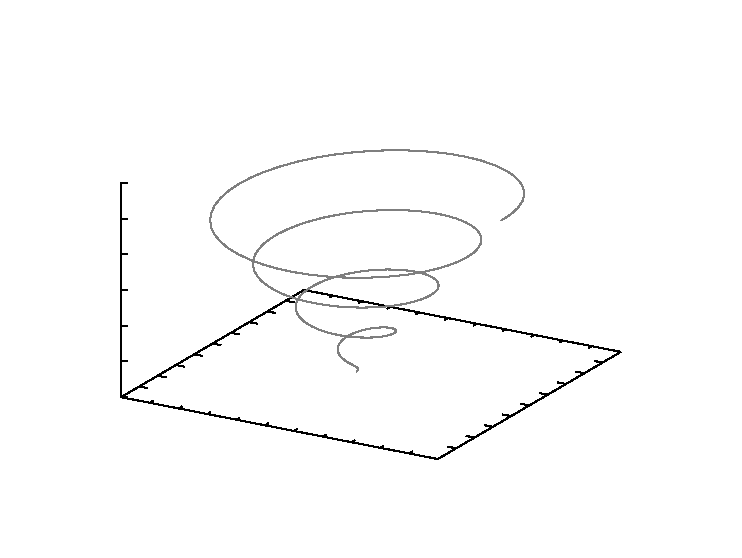
\includegraphics{fig451}}%
    \gplfronttext
  \end{picture}%
\endgroup

  \end{center}
  \caption[]{\quad Conical helix $C$}
  \label{fig:conhelix}
 \end{figure}
\end{exmp}\smallskip
\hrule width \textwidth height 0.5pt
\begin{exmp}
 Let $\mathbf{f}(x,y,z) = x\,\mathbf{i} + y\,\mathbf{j} + 2z\,\mathbf{k}$ be a vector field in $\Real{3}$.
 Using the same curve $C$ from Example \ref{exmp:conhelix}, evaluate $\lineintvec{C}{f}{r}$.\smallskip
 \par\noindent \emph{Solution:} Note that $F(x,y,z)=\frac{x^2}{2}+\frac{y^2}{2}+z^2$ is a potential for
 $\mathbf{f}(x,y,z)$ (i.e. $\nabla F = \mathbf{f}$). So by Theorem \ref{thm:lineintsuffpath3} we know that
 \begin{align*}
  \lineintvec{C}{f}{r} ~&=~ F(B) ~-~ F(A) ~~,~\text{where $A=(x(0),y(0),z(0))$ and $B=(x(8\pi),y(8\pi),z(8\pi))$, so}\\
   &=~ F(8\pi\sin 8\pi,8\pi\cos 8\pi,8\pi) ~-~ F(0\sin 0,0\cos 0,0)\\
   &=~ F(0,8\pi,8\pi) ~-~ F(0,0,0)\\
   &=~ 0+\frac{(8\pi)^2}{2} + (8\pi)^2 - (0+0+0)
   ~=~ 96\pi^2 ~.
 \end{align*}
\end{exmp}
\hrule width \textwidth height 0.5pt
\medskip

We will now discuss a generalization of Green's Theorem in $\Real{2}$ to \emph{orientable} surfaces in $\Real{3}$,
called \emph{Stokes' Theorem}.\index{Stokes' Theorem}\index{orientable}\index{surface!orientable} A surface $\Sigma$ in
$\Real{3}$ is \textbf{orientable} if there is a continuous vector field $\mathbf{N}$ in $\Real{3}$ such that
$\mathbf{N}$ is nonzero and normal to $\Sigma$ (i.e. perpendicular to the tangent plane) at each point of $\Sigma$. We say
that such an $\mathbf{N}$ is a \emph{normal vector field}.\index{normal vector field}\index{vector
field!normal}

\piccaption[]{}\parpic[r]{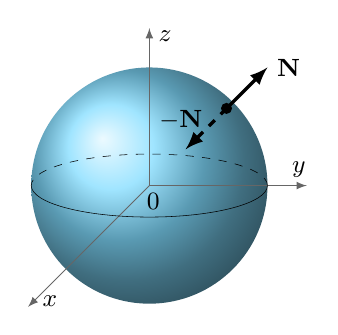
\begin{tikzpicture}
 \usetikzlibrary{arrows}
 \definecolor{spherecolor}{HTML}{80DCFF}
 \shade [ball color=spherecolor] (0,0) circle (1.5);
 \draw [black!60,line width=0.3pt,-latex] (0,0) -- (2,0,0);
 \draw [black!60,line width=0.3pt,-latex] (0,0) -- (0,2,0);
 \draw [black!60,line width=0.3pt,-latex] (0,0) -- (0,0,4);
 \pgfputat{\pgfpointxyz{1.9}{0.2}{0}}{\pgfbox[center,center]{\small $y$}};
 \pgfputat{\pgfpointxyz{0.2}{1.9}{0}}{\pgfbox[center,center]{\small $z$}};
 \pgfputat{\pgfpointxyz{0.2}{0}{3.8}}{\pgfbox[center,center]{\small $x$}};
 \pgfputat{\pgfpointxyz{0.05}{-0.2}{0}}{\pgfbox[center,center]{\small $0$}};
 \draw [line width=0.2pt] (-1.5,0) arc (180:360:1.5 and 0.4);
 \draw [dashed,line width=0.2pt] (1.5,0) arc (0:180:1.5 and 0.4);
 \fill (0.98,0.98) circle (2pt);
 \draw [line width=1.2pt,-latex] (0.98,0.98) -- (1.5,1.5);
 \node [right] at (1.5,1.5) {\small $\mathbf{N}$};
 \draw [dashed,line width=1.2pt,-latex] (0.98,0.98) -- (0.46,0.46);
 \node [above] at (0.4,0.58) {\small $-\mathbf{N}$};
\end{tikzpicture}}
For example, the unit sphere $x^2 + y^2 + z^2 = 1$ is orientable, since the continuous vector field
$\mathbf{N}(x,y,z) = x\,\mathbf{i} + y\,\mathbf{j} + z\,\mathbf{k}$ is nonzero and normal to the sphere at each point.
In fact, $-\mathbf{N}(x,y,z)$ is another normal vector field (see Figure 4.5.2). We see in this case that
$\mathbf{N}(x,y,z)$ is what we have called an outward normal vector, and $-\mathbf{N}(x,y,z)$ is an \emph{inward} normal
vector. These ``outward'' and ``inward'' normal vector fields on the sphere correspond to an ``outer'' and
``inner'' side, respectively, of the sphere.
That is, we say that the sphere is a \emph{two-sided} surface.\index{surface!two-sided}
Roughly, ``two-sided'' means ``orientable''.
Other examples of two-sided, and hence orientable, surfaces are
cylinders, paraboloids, ellipsoids, and planes.

You may be wondering what kind of surface would \emph{not} have two sides. An example is the
\textbf{M\"{o}bius strip},\index{moebius@M\"{o}bius strip} which is constructed by taking a thin rectangle and
connecting its ends at the opposite corners, resulting in a ``twisted'' strip
(see Figure \ref{fig:mobius}).

\begin{figure}[h]
 \centering
 \subfloat[][Connect $A$ to $A$ and $B$ to $B$ along the ends]{
  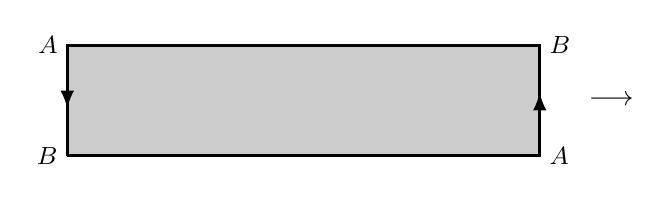
\begin{tikzpicture}
   \usetikzlibrary{arrows}
   \filldraw [black,line width=1.2pt,fill=black!20] (0,0) -- (6,0) -- (6,1.4) -- (0,1.4) -- (0,0);
   \draw [black,line width=1.2pt,-latex] (0,1.4) -- (0,0.6);
   \draw [black,line width=1.2pt,-latex] (6,0) -- (6,0.8);
   \node [left] at (0,1.4) {\small $A$};
   \node [left] at (0,0) {\small $B$};
   \node [right] at (6,0) {\small $A$};
   \node [right] at (6,1.4) {\small $B$};
   \node [right] at (6.5,0.7) {$\longrightarrow$};
  \end{tikzpicture}}
 \quad
 \subfloat[][Not orientable]{
  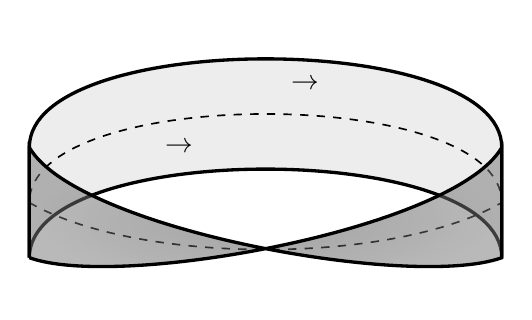
\begin{tikzpicture}
   \usetikzlibrary{arrows}
   \filldraw [black,line width=1.2pt,fill=black!7] (0,1.4) -- (0,0) to[controls=+(90:1.5) and +(90:1.5)] (6,0) --
    (6,1.4) to[controls=+(90:1.5) and +(90:1.5)] (0,1.4);
   \draw [dashed,black,line width=0.6pt] (0,0.7) to[out=-30,in=210,looseness=0.68] (6,0.7)
    to[controls=+(90:1.5) and +(90:1.5)] (0,0.7);
   \filldraw [fill opacity=0.3,black,line width=1.2pt,shading=radial,outer color=black!20,inner color=black!50] (0,0) -- (0,1.4)
    to[out=-60,in=200,looseness=0.5] (6,0) -- (6,1.4) to[out=240,in=-20,looseness=0.5] (0,0);
   \node [above] at (3,1.7) {\small\PHpedestrian};
   \node at (3.5,2.2) {$\rightarrow$};
   \node [below,rotate=-180,cm={-1,0,0,1,(0,0)}] at (2.4,1.0) {\small\PHpedestrian};
   \node at (1.9,1.4) {$\rightarrow$};
  \end{tikzpicture}}
 \caption[]{\quad M\"{o}bius strip}
 \label{fig:mobius}
\end{figure}

If you imagine walking along a line down the center of the M\"{o}bius strip, as in Figure \ref{fig:mobius}(b), then
you arrive back at the same place from which you started but upside down! That is, your \emph{orientation} changed
even though your motion was continuous along that center line. Informally, thinking of your vertical direction as a
normal vector field along the strip, there is a discontinuity at your starting point (and, in fact, at every
point) since your vertical direction takes two different values there. The M\"{o}bius strip has only \emph{one side},
and hence is nonorientable.\footnote{For further discussion of orientability, see \cite[\S\,IV.7]{one}.}

For an orientable surface $\Sigma$ which has a boundary curve $C$, pick a unit normal vector $\mathbf{n}$
such that if you walked along $C$ with your head pointing in the direction of $\mathbf{n}$, then the surface would be on
your left. We say in this situation that $\mathbf{n}$ is a \emph{positive unit normal vector}\index{vector!positive unit
normal} and that $C$ is traversed \emph{$\mathbf{n}$-positively}\index{n-positive@$\mathbf{n}$-positive direction}. We can
now state Stokes' Theorem:

\statethm{thm:stokes}{
 {(\textbf{Stokes' Theorem})\,\index{Stokes' Theorem}
  Let $\Sigma$ be an orientable surface in $\Real{3}$ whose boundary is a simple closed curve $C$, and let
  $\mathbf{f}(x,y,z) = P(x,y,z) \mathbf{i} + Q(x,y,z) \mathbf{j} + R(x,y,z) \mathbf{k}$ be a smooth vector field
  defined on some subset of $\Real{3}$ that contains $\Sigma$. Then
  \begin{equation}\label{eqn:stokes}
   \olineintvec{C}{f}{r} ~=~ \iint\limits_{\Sigma} \Dotprod{(\text{curl}~{\mathbf{f}}\,)}{\mathbf{n}}\,d\sigma ~,
  \end{equation}
  where
  \begin{equation}\label{eqn:curl}
   \text{curl}~\mathbf{f} ~=~ \left( \frac{\partial R}{\partial y} - \frac{\partial Q}{\partial z} \right) \mathbf{i} ~+~
    \left( \frac{\partial P}{\partial z} - \frac{\partial R}{\partial x} \right) \mathbf{j} ~+~
    \left( \frac{\partial Q}{\partial x} - \frac{\partial P}{\partial y} \right) \mathbf{k} ~,\index{curl}
  \end{equation}
  $\mathbf{n}$ is a positive unit normal vector over $\Sigma$, and $C$ is traversed $\mathbf{n}$-positively.}
}

\begin{proofbar}
\begin{proof}[Proof:]
 As the general case is beyond the scope of this text, we will prove the theorem only for the special case where
 $\Sigma$ is the graph of $z=z(x,y)$ for some smooth real-valued function $z(x,y)$, with $(x,y)$ varying over a region
 $D$ in $\Real{2}$. \piccaption[]{}\parpic[r]{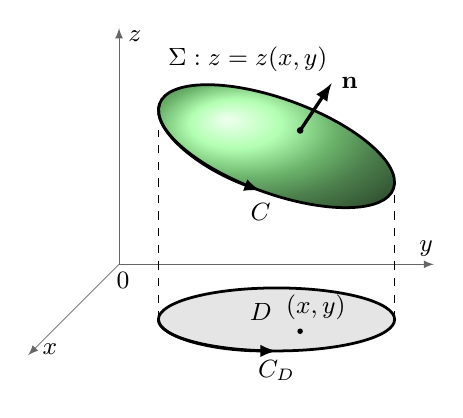
\begin{tikzpicture}
  \usetikzlibrary{arrows}
  \shade [ball color=green!40] [rotate around={-20:(2.0,1.5)}] (2.0,1.5) ellipse (1.58 and 0.6);
  \draw [black!60,line width=0.3pt,-latex] (0,0) -- (4,0,0);
  \draw [black!60,line width=0.3pt,-latex] (0,0) -- (0,3,0);
  \draw [black!60,line width=0.3pt,-latex] (0,0) -- (0,0,3);
  \pgfputat{\pgfpointxyz{3.9}{0.2}{0}}{\pgfbox[center,center]{\small $y$}};
  \pgfputat{\pgfpointxyz{0.2}{2.9}{0}}{\pgfbox[center,center]{\small $z$}};
  \pgfputat{\pgfpointxyz{0.2}{0}{2.8}}{\pgfbox[center,center]{\small $x$}};
  \pgfputat{\pgfpointxyz{0.05}{-0.2}{0}}{\pgfbox[center,center]{\small $0$}};
  \filldraw [black,line width=1pt,fill=black!10] (2,-0.7) ellipse (1.5 and 0.4);
  \draw [line width=1pt,-latex] (0.5,-0.7) arc (180:270:1.5 and 0.4);
  \draw [rotate around={-20:(2.0,1.5)},line width=1pt] (2.0,1.5) ellipse (1.58 and 0.6);
  \draw [rotate around={-20:(2.0,1.5)},line width=1pt,-latex] (0.42,1.5) arc (180:270:1.58 and 0.6);
  \fill (2.3,-0.85) circle (1pt);
  \fill (2.3,1.7) circle (1.2pt);
  \draw [line width=1.2,-latex] (2.3,1.7) -- (2.7,2.3);
  \node [right] at (2.7,2.3) {\small $\mathbf{n}$};
  \node [above] at (2.5,-0.83) {\small $(x,y)$};
  \node at (1.8,-0.6) {\small $D$};
  \node [below] at (2,-1.1) {\small $C_D$};
  \node [below] at (1.8,0.9) {\small $C$};
  \node [right] at (0.5,2.6) {\small $\Sigma: z = z(x,y)$};
  \draw [dashed] (0.5,-0.7) -- (0.5,1.7);
  \draw [dashed] (3.5,-0.7) -- (3.5,1);
 \end{tikzpicture}}
 Projecting $\Sigma$ onto the $xy$-plane, we see that the closed curve $C$ (the boundary curve of $\Sigma$) projects
 onto a closed curve $C_D$ which is the boundary curve of $D$ (see Figure 4.5.4). Assuming that $C$ has a smooth
 parametrization, its projection $C_D$ in the $xy$-plane also has a smooth parametrization, say
 \begin{displaymath}
  C_D:~ x=x(t)~,~ y=y(t)~,~ a \le t \le b ~,
 \end{displaymath}
 and so $C$ can be parametrized (in $\Real{3}$) as
 \begin{displaymath}
  C:~ x=x(t)~,~ y=y(t)~,~ z=z(x(t),y(t))~,~a \le t \le b ~,
 \end{displaymath}
 since the curve $C$ is part of the surface $z=z(x,y)$. Now, by the Chain Rule (Theorem \ref{thm:multichain}), for $z=z(x(t),y(t))$ as a function of $t$, we know that
 \begin{displaymath}
  z\,'(t) ~=~ \frac{\partial z}{\partial x}\,x\,'(t) ~+~ \frac{\partial z}{\partial y}\,y\,'(t) ~,
 \end{displaymath}
 and so
 \begin{align*}
  \olineintvec{C}{f}{r} ~&=~ \int_C P(x,y,z)\,dx + Q(x,y,z)\,dy + R(x,y,z)\,dz\\
   &=~ \int_a^b \left( P\,x\,'(t) + Q\,y\,'(t) +
    R\left( \frac{\partial z}{\partial x}\,x\,'(t) + \frac{\partial z}{\partial y}\,y\,'(t)
    \right) \right)\,dt\\
   &=~ \int_a^b \left( \left( P+R\,\frac{\partial z}{\partial x} \right) x\,'(t) +
    \left( Q+R\,\frac{\partial z}{\partial y} \right) y\,'(t) \right)\,dt\\
   &=~ \int_{C_D} \tilde{P}(x,y)\,dx + \tilde{Q}(x,y)\,dy ~,
 \end{align*}
 where
 \begin{align*}
  \tilde{P}(x,y) ~&=~ P(x,y,z(x,y)) ~+~ R(x,y,z(x,y))\,\frac{\partial z}{\partial x}(x,y)~,\text{and}\\
  \tilde{Q}(x,y) ~&=~ Q(x,y,z(x,y)) ~+~ R(x,y,z(x,y))\,\frac{\partial z}{\partial y}(x,y)
 \end{align*}
 for $(x,y)$ in $D$. Thus, by Green's Theorem applied to the region $D$, we have
 \begin{equation}\label{eqn:stokesproof}
  \olineintvec{C}{f}{r} ~=~ \iint\limits_{D} \left( \frac{\partial \tilde{Q}}{\partial x} -
   \frac{\partial \tilde{P}}{\partial y} \right)\,dA ~.
 \end{equation}
 Thus,
 \begin{align*}
  \frac{\partial \tilde{Q}}{\partial x} ~&=~ \frac{\partial}{\partial x} \left( Q(x,y,z(x,y)) +
   R(x,y,z(x,y))\,\frac{\partial z}{\partial y}(x,y) \right) ~,~\text{so by the Product Rule we get}\\
   &=~ \frac{\partial}{\partial x} \left( Q(x,y,z(x,y)) \right) + \left( \frac{\partial}{\partial x} R(x,y,z(x,y))
   \right) \frac{\partial z}{\partial y}(x,y) + R(x,y,z(x,y))\,\frac{\partial}{\partial x} \left(
   \frac{\partial z}{\partial y}(x,y) \right) ~.
 \end{align*}
 Now, by formula (\ref{eqn:chainrule3x}) in Theorem \ref{thm:chainrule3}, we have
 \begin{align*}
  \frac{\partial}{\partial x} \left( Q(x,y,z(x,y)) \right) ~&=~
   \frac{\partial Q}{\partial x}\,\frac{\partial x}{\partial x} ~+~
   \frac{\partial Q}{\partial y}\,\frac{\partial y}{\partial x} ~+~
   \frac{\partial Q}{\partial z}\,\frac{\partial z}{\partial x}\\
   &=~ \frac{\partial Q}{\partial x} \cdot 1 ~+~ \frac{\partial Q}{\partial y} \cdot 0 ~+~ \frac{\partial Q}{\partial z}\,
    \frac{\partial z}{\partial x}\\
   &=~ \frac{\partial Q}{\partial x} ~+~ \frac{\partial Q}{\partial z}\,\frac{\partial z}{\partial x} ~.\\
  \intertext{Similarly,}
  \frac{\partial}{\partial x} \left( R(x,y,z(x,y)) \right) ~&=~
   \frac{\partial R}{\partial x} ~+~ \frac{\partial R}{\partial z}\,\frac{\partial z}{\partial x} ~.
\end{align*}
 Thus,
 \begin{align*}
  \frac{\partial \tilde{Q}}{\partial x} ~&=~ \frac{\partial Q}{\partial x} ~+~ \frac{\partial Q}{\partial z}\,
   \frac{\partial z}{\partial x} ~+~ \left( \frac{\partial R}{\partial x} + \frac{\partial R}{\partial z}\,
   \frac{\partial z}{\partial x} \right) \frac{\partial z}{\partial y} ~+~ R(x,y,z(x,y))\,
   \frac{\partial^2 z}{\partial x \, \partial y}\\
   &=~ \frac{\partial Q}{\partial x} ~+~ \frac{\partial Q}{\partial z}\,\frac{\partial z}{\partial x} ~+~
    \frac{\partial R}{\partial x}\,\frac{\partial z}{\partial y} ~+~ \frac{\partial R}{\partial z}\,
    \frac{\partial z}{\partial x}\,\frac{\partial z}{\partial y} ~+~ R\,\frac{\partial^2 z}{\partial x \, \partial y}~.\\
  \intertext{In a similar fashion, we can calculate}
  \frac{\partial \tilde{P}}{\partial y} ~&=~ \frac{\partial P}{\partial y} ~+~
   \frac{\partial P}{\partial z}\,\frac{\partial z}{\partial y} ~+~
    \frac{\partial R}{\partial y}\,\frac{\partial z}{\partial x} ~+~ \frac{\partial R}{\partial z}\,
    \frac{\partial z}{\partial y}\,\frac{\partial z}{\partial x} ~+~ R\,\frac{\partial^2 z}{\partial y \, \partial x}~.
 \end{align*}
 So subtracting gives
 \begin{equation}\label{eqn:stokeslong}
  \frac{\partial \tilde{Q}}{\partial x} ~-~ \frac{\partial \tilde{P}}{\partial y} ~=~
   \left( \frac{\partial Q}{\partial z} - \frac{\partial R}{\partial y} \right) \frac{\partial z}{\partial x}
   ~+~ \left( \frac{\partial R}{\partial x} - \frac{\partial P}{\partial z}\right) \frac{\partial z}{\partial y}
   ~+~ \left( \frac{\partial Q}{\partial x} - \frac{\partial P}{\partial y} \right)
 \end{equation}
 since $\frac{\partial^2 z}{\partial x \, \partial y} = \frac{\partial^2 z}{\partial y \, \partial x}$ by the
 smoothness of $z=z(x,y)$. Hence, by equation (\ref{eqn:stokesproof}),
 \begin{equation}\label{eqn:stokespart1}
  \olineintvec{C}{f}{r} ~=~ \iint\limits_{D} \left(
   -\left( \frac{\partial R}{\partial y} - \frac{\partial Q}{\partial z} \right) \frac{\partial z}{\partial x}
   -\left( \frac{\partial P}{\partial z} - \frac{\partial R}{\partial x} \right) \frac{\partial z}{\partial y}
   + \left( \frac{\partial Q}{\partial x} - \frac{\partial P}{\partial y} \right) \right)\,dA
 \end{equation}
 after factoring out a $-1$ from the terms in the first two products in equation (\ref{eqn:stokeslong}).
 
 \picskip{0}
 Now, recall from Section 2.3 (see p.76) that the vector $\mathbf{N} = -\frac{\partial z}{\partial x}\,\mathbf{i} -
 \frac{\partial z}{\partial y}\,\mathbf{j} + \mathbf{k}$ is normal to the tangent plane to the surface $z=z(x,y)$ at
 each point of $\Sigma$. Thus,
 \begin{displaymath}
  \mathbf{n} ~=~ \frac{\mathbf{N}}{\Norm{\mathbf{N}}} ~=~
   \frac{-\frac{\partial z}{\partial x}\,\mathbf{i} - \frac{\partial z}{\partial y}\,\mathbf{j} +
   \mathbf{k}}{\sqrt{1 + \left( \tfrac{\partial z}{\partial x} \right)^2 +
   \left( \tfrac{\partial z}{\partial y} \right)^2}}
 \end{displaymath}
 is in fact a positive unit normal vector to $\Sigma$ (see Figure 4.5.4). Hence, using the parametrization
 $\mathbf{r}(x,y) = x\,\mathbf{i} + y\,\mathbf{j} + z(x,y)\,\mathbf{k}$, for $(x,y)$ in $D$, of the surface $\Sigma$,
 we have $\frac{\partial \mathbf{r}}{\partial x} = \mathbf{i} + \frac{\partial z}{\partial x}\,\mathbf{k}$ and
 $\frac{\partial \mathbf{r}}{\partial y} = \mathbf{j} + \frac{\partial z}{\partial y}\,\mathbf{k}$, and so
 $\Norm{\Crossprod{\frac{\partial \mathbf{r}}{\partial x}}{\frac{\partial \mathbf{r}}{\partial y}}} =
   \sqrt{1 + \left( \tfrac{\partial z}{\partial x} \right)^2 + \left( \tfrac{\partial z}{\partial y} \right)^2}$.
 So we see that using formula (\ref{eqn:curl}) for $\text{curl}~{\mathbf{f}}$, we have
 \begin{align*}
  \iint\limits_{\Sigma} \Dotprod{(\text{curl}~{\mathbf{f}})}{\mathbf{n}}\,d\sigma ~&=~
   \iint\limits_{D} \Dotprod{(\text{curl}~{\mathbf{f}}\,)}{\mathbf{n}}\,
   \NORM{\Crossprod{\frac{\partial \mathbf{r}}{\partial x}}{\frac{\partial \mathbf{r}}{\partial y}}}\,dA\\
   &=~ \iint\limits_{D} \Dotprod{\left( \left( \frac{\partial R}{\partial y} - \frac{\partial Q}{\partial z} \right)
    \mathbf{i} + \left( \frac{\partial P}{\partial z} - \frac{\partial R}{\partial x} \right) \mathbf{j} +
    \left( \frac{\partial Q}{\partial x} - \frac{\partial P}{\partial y} \right) \mathbf{k}
    \right)}{\left( -\frac{\partial z}{\partial x}\mathbf{i} - \frac{\partial z}{\partial y}\mathbf{j} +
    \mathbf{k} \right)} dA\\
   &=~ \iint\limits_{D} \left(
    -\left( \frac{\partial R}{\partial y} - \frac{\partial Q}{\partial z} \right) \frac{\partial z}{\partial x}
    -\left( \frac{\partial P}{\partial z} - \frac{\partial R}{\partial x} \right) \frac{\partial z}{\partial y}
    + \left( \frac{\partial Q}{\partial x} - \frac{\partial P}{\partial y} \right) \right)\,dA ~,
 \end{align*}
 which, upon comparing to equation (\ref{eqn:stokespart1}), proves the Theorem.
 
\end{proof}\end{proofbar}

Note: 
The condition in Stokes' Theorem that the surface $\Sigma$ have a (continuously varying) positive unit normal
vector $\mathbf{n}$ and a boundary curve $C$ traversed $\mathbf{n}$-positively can be expressed more precisely as follows:
if $\mathbf{r}(t)$ is the position vector for $C$ and $\mathbf{T}(t) = \mathbf{r}\,'(t)/\norm{\mathbf{r}\,'(t)}$
is the unit tangent vector to $C$, then the vectors $\mathbf{T}$, $\mathbf{n}$, $\Crossprod{\mathbf{T}}{\mathbf{n}}$ form a
right-handed system.

Also, it should be noted that Stokes' Theorem holds even when the boundary curve $C$ is piecewise smooth.


\medskip
\hrule width \textwidth height 0.5pt
\begin{exmp}\label{exmp:stokesparab}
 Verify Stokes' Theorem for $\mathbf{f}(x,y,z) = z\,\mathbf{i} + x\,\mathbf{j} + y\,\mathbf{k}$ when $\Sigma$ is the
 paraboloid $z=x^2 + y^2$ such that $z \le 1$ (see Figure 4.5.5).
 \smallskip
 \piccaption[]{\quad $z=x^2 + y^2$}\parpic[r]{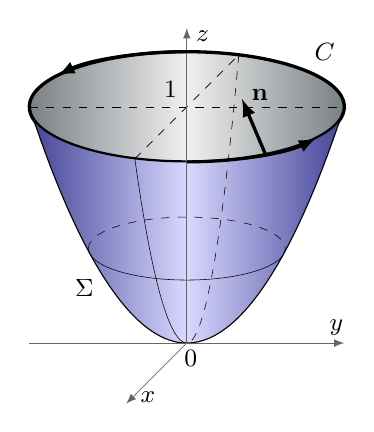
\begin{tikzpicture}
  \usetikzlibrary{arrows}
  \definecolor{insideo}{HTML}{798084}
  \definecolor{insidei}{HTML}{F0F0F0}
  \definecolor{outer}{HTML}{424296}
  \definecolor{inner}{HTML}{D8D8FF}
  \shadedraw [left color=insideo,right color=insideo,middle color=insidei,line width=1.2pt] (0,3) ellipse (2 and 0.7);
  \shadedraw [left color=outer,right color=outer,middle color=inner]
  (2,3) arc (360:180:2 and 0.7) -- (-2,3) parabola bend (0,0) (2,3);
  \draw [dashed,line width=0.2pt] (-2,3) -- (2,3);
  \draw [dashed,line width=0.2pt] (-0.66,2.34) -- (0.66,3.66);
  \draw [line width=0.2pt] (-0.66,2.34) parabola [bend at end] (0,0);
  \draw [dashed,line width=0.2pt] (0.66,3.66) parabola [bend at end] (0,0);
  \draw [line width=0.2pt] (-1.25,1.2) arc (180:360:1.25 and 0.4);
  \draw [dashed,line width=0.2pt] (-1.25,1.2) arc (180:0:1.25 and 0.4);
  \draw [black!60,line width=0.3pt,-latex] (-2,0) -- (2,0,0);
  \draw [black!60,line width=0.3pt,-latex] (0,0) -- (0,4,0);
  \draw [black!60,line width=0.3pt,-latex] (0,0) -- (0,0,2);
  \draw [black,line width=1.1pt,-latex] (0,2.3) arc (270:325:2 and 0.7);
  \draw [black,line width=1.1pt,-latex] (0,3.7) arc (90:145:2 and 0.7);
  \draw [black,line width=1.2pt,-latex] (1,2.3938) -- (0.7,3.1);
  \pgfputat{\pgfpointxyz{1.9}{0.2}{0}}{\pgfbox[center,center]{\small $y$}};
  \pgfputat{\pgfpointxyz{0.2}{3.9}{0}}{\pgfbox[center,center]{\small $z$}};
  \pgfputat{\pgfpointxyz{0.2}{0}{1.8}}{\pgfbox[center,center]{\small $x$}};
  \pgfputat{\pgfpointxyz{0.05}{-0.2}{0}}{\pgfbox[center,center]{\small $0$}};
  \node [right] at (0.7,3.15) {\small $\mathbf{n}$};
  \node [right] at (1.5,3.7) {\small $C$};
  \node at (-1.3,0.7) {\small $\Sigma$};
  \node [above left] at (0,3) {\small $1$};
 \end{tikzpicture}
 }
 \par\noindent\emph{Solution:} The positive unit normal vector to the surface\\$z=z(x,y)=x^2 + y^2$ is
 \begin{displaymath}
  \mathbf{n} ~=~
   \frac{-\frac{\partial z}{\partial x}\,\mathbf{i} - \frac{\partial z}{\partial y}\,\mathbf{j} +
   \mathbf{k}}{\sqrt{1 + \left( \tfrac{\partial z}{\partial x} \right)^2 +
   \left( \tfrac{\partial z}{\partial y} \right)^2}} ~=~
   \frac{-2x\,\mathbf{i} - 2y\,\mathbf{j} + \mathbf{k}}{\sqrt{1 + 4x^2 + 4y^2}} ~,
 \end{displaymath}
 and $\text{curl}~\mathbf{f}= (1-0)\,\mathbf{i}+(1-0)\,\mathbf{j}+(1-0)\,\mathbf{k} = \mathbf{i}+\mathbf{j}+\mathbf{k}$,
 so
 \begin{displaymath}
  \Dotprod{(\text{curl}~{\mathbf{f}}\,)}{\mathbf{n}} ~=~ (-2x-2y+1)/\sqrt{1 + 4x^2 + 4y^2} ~.
 \end{displaymath}
 
 \par\noindent
 Since $\Sigma$ can be parametrized as $\mathbf{r}(x,y) = x\,\mathbf{i}+y\,\mathbf{j}+(x^2 + y^2 )\,\mathbf{k}$ for
 $(x,y)$ in the region $D = \lbrace \, (x,y):\,x^2 + y^2 \le 1 \,\rbrace$, then
 \begin{align*}
  \iint\limits_{\Sigma} \Dotprod{(\text{curl}~{\mathbf{f}}\,)}{\mathbf{n}}\,d\sigma ~&=~
   \iint\limits_{D} \Dotprod{(\text{curl}~{\mathbf{f}}\,)}{\mathbf{n}}\,
   \NORM{\Crossprod{\frac{\partial \mathbf{r}}{\partial x}}{\frac{\partial \mathbf{r}}{\partial y}}}\,dA\\
   &=~ \iint\limits_{D} \frac{-2x-2y+1}{\sqrt{1 + 4x^2 + 4y^2}}\,\sqrt{1 + 4x^2 + 4y^2}\,dA\\
   &=~ \iint\limits_{D} (-2x-2y+1)\,dA ~,~\text{so switching to polar coordinates gives}\\
   &=~ \int_0^{2\pi} \int_0^1 (-2r\cos \theta - 2r\sin \theta + 1)r\,dr\,d\theta\\
   &=~ \int_0^{2\pi} \int_0^1 (-2r^2 \cos \theta - 2r^2 \sin \theta + r)\,dr\,d\theta\\
   &=~ \int_0^{2\pi} \left( -\tfrac{2r^3}{3} \cos \theta - \tfrac{2r^3}{3} \sin \theta +
   \tfrac{r^2}{2}\,\Big|_{r=0}^{r=1} \,\right)\,d\theta\\
   &=~ \int_0^{2\pi} \left( -\tfrac{2}{3} \cos \theta - \tfrac{2}{3} \sin \theta + \tfrac{1}{2} \right)\,d\theta\\
   &=~ -\tfrac{2}{3} \sin \theta + \tfrac{2}{3} \cos \theta + \tfrac{1}{2}\theta\,\Big|_0^{2\pi} ~=~ \pi ~.
 \end{align*}
 
\picskip{0} 

 The boundary curve $C$ is the unit circle $x^2 + y^2 =1$ laying in the plane $z=1$ (see Figure 4.5.5), which can be
 parametrized as $x = \cos t$, $y = \sin t$, $z = 1$ for $0 \le t \le 2\pi$. So
 \begin{align*}
  \olineintvec{C}{f}{r} ~&=~ \int_0^{2\pi} ((1)(-\sin t) + (\cos t)(\cos t) + (\sin t)(0))\,dt\\
   &=~ \int_0^{2\pi} \left( -\sin t + \frac{1+\cos 2t}{2} \right) \,dt \quad \left( \text{here we used $\cos^2 t =
   \frac{1+\cos 2t}{2}$} \right)\\
   &=~ \cos t + \frac{t}{2} + \frac{\sin 2t}{4}\,\Big|_0^{2\pi} ~=~ \pi ~.
 \end{align*}
 So we see that 
 \[\olineintvec{C}{f}{r}=\iint_{\Sigma} \Dotprod{(\text{curl}~{\mathbf{f}}\,)}{\mathbf{n}}
 \,d\sigma,\] as predicted by Stokes' Theorem.
\end{exmp}
\hrule width \textwidth height 0.5pt
\medskip

The line integral in the preceding example was far simpler to calculate than the surface integral, but this will not
always be the case.

\medskip
\hrule width \textwidth height 0.5pt
\begin{exmp}
 Let $\Sigma$ be the elliptic paraboloid $z=\frac{x^2}{4}+\frac{y^2}{9}$ for $z \le 1$, and let $C$ be its boundary
 curve.
 Calculate $\olineintvec{C}{f}{r}$ for $\mathbf{f}(x,y,z)=(9xz+2y)\mathbf{i}+(2x+y^2 )\mathbf{j}+(-2y^2 +2z)\mathbf{k}$,
 where $C$ is traversed counterclockwise.\smallskip
 \par\noindent\emph{Solution:} The surface is similar to the one in Example \ref{exmp:stokesparab}, except now the
 boundary curve $C$ is the ellipse $\frac{x^2}{4}+\frac{y^2}{9}=1$ laying in the plane $z=1$. 
 In this case, using Stokes' Theorem is easier than computing the line integral directly. 
 As in Example \ref{exmp:stokesparab}, at each
 point $(x,y,z(x,y))$ on the surface $z=z(x,y)=\frac{x^2}{4}+\frac{y^2}{9}$ the vector
 \begin{displaymath}
  \mathbf{n} ~=~
   \frac{-\frac{\partial z}{\partial x}\,\mathbf{i} - \frac{\partial z}{\partial y}\,\mathbf{j} +
   \mathbf{k}}{\sqrt{1 + \left( \tfrac{\partial z}{\partial x} \right)^2 +
   \left( \tfrac{\partial z}{\partial y} \right)^2}} ~=~
   \frac{-\tfrac{x}{2}\,\mathbf{i} - \tfrac{2y}{9}\,\mathbf{j} + \mathbf{k}}{\sqrt{1 +\tfrac{x^2}{4}+
    \tfrac{4y^2}{9}}} ~,
 \end{displaymath}
 is a positive unit normal vector to $\Sigma$. And calculating the curl of $\mathbf{f}$ gives
 \begin{displaymath}
  \text{curl}~\mathbf{f} ~=~ (-4y-0)\mathbf{i} ~+~ (9x-0)\mathbf{j} ~+~ (2-2)\mathbf{k} ~=~ -4y\,\mathbf{i} ~+~ 9x\,\mathbf{j} ~+~
   0\,\mathbf{k}~,
 \end{displaymath}
 so
 \begin{displaymath}
  \Dotprod{(\text{curl}~{\mathbf{f}}\,)}{\mathbf{n}} ~=~ \frac{(-4y)(-\tfrac{x}{2})+(9x)(-\tfrac{2y}{9})+
   (0)(1)}{\sqrt{1 +\tfrac{x^2}{4}+\tfrac{4y^2}{9}}} ~=~ \frac{2xy-2xy+0}{\sqrt{1 +\tfrac{x^2}{4}+\tfrac{4y^2}{9}}} ~=~ 0~,
 \end{displaymath}
 and so by Stokes' Theorem
 \begin{displaymath}
  \olineintvec{C}{f}{r} ~=~ \iint\limits_{\Sigma} \Dotprod{(\text{curl}~{\mathbf{f}}\,)}{\mathbf{n}}\,d\sigma ~=~
   \iint\limits_{\Sigma} 0\,d\sigma ~=~ 0 ~.
 \end{displaymath}
\end{exmp}
\hrule width \textwidth height 0.5pt
\smallskip
In physical applications, for a simple closed curve $C$ the line integral $\olineintvec{C}{f}{r}$
is often called the \textbf{circulation}\index{circulation} of $\mathbf{f}$ around $C$. For example, if $\mathbf{E}$
represents the electrostatic field due to a point charge, then
it turns out\footnote{See Ch. 2 in \cite{rmc}.} that $\text{curl}~\mathbf{E} = \mathbf{0}$, which means that the
circulation $\olineintvec{C}{E}{r}=0$ by Stokes' Theorem. Vector fields which have zero curl are often called
\emph{irrotational}\index{irrotational} fields.

In fact, the term curl was created by the 19\textsuperscript{th} century Scottish physicist James Clerk Maxwell in his
study of electromagnetism, where it is used extensively. In physics, the curl is interpreted as a measure of
\emph{circulation density}. This is best seen by using another definition of curl $\mathbf{f}$ which is
equivalent\footnote{See \cite{sch}, p. 78--81, for the derivation.} to the definition given by
formula (\ref{eqn:curl}). Namely, for a point $(x,y,z)$ in $\Real{3}$,
\begin{equation}\label{eqn:curlalt}
 \Dotprod{\mathbf{n}}{(\text{curl}~\mathbf{f}\,)}(x,y,z) ~=~ \lim_{S \to 0} \frac{1}{S} \olineintvec{C}{f}{r} ~,
\end{equation}
where $S$ is the surface area of a surface $\Sigma$ containing the point $(x,y,z)$ and with a simple closed boundary
curve $C$ and positive unit normal vector $\mathbf{n}$ at $(x,y,z)$. In the limit, think of the curve $C$ shrinking to
the point $(x,y,z)$, which causes $\Sigma$, the surface it bounds, to have smaller and smaller surface area. That ratio
of circulation to surface area in the limit is what makes the curl a rough measure of circulation density (i.e.
circulation per unit area).

\piccaption[]{\quad Curl and rotation}\parpic[r]{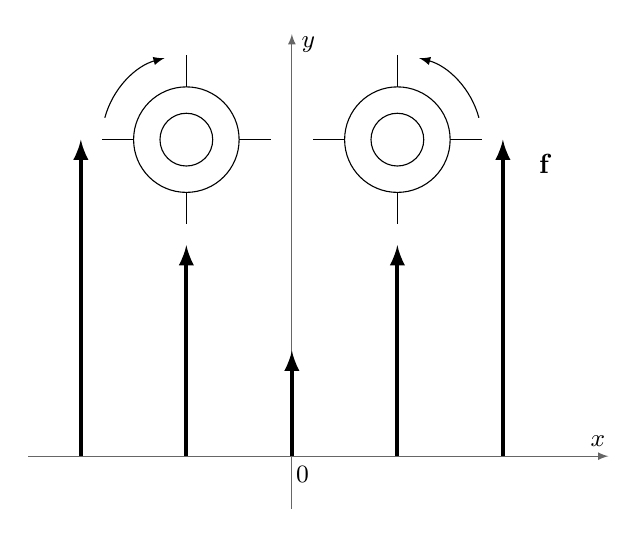
\begin{tikzpicture}[scale=1.34]
 \usetikzlibrary{arrows}
 \draw [black!60,line width=0.3pt,-latex] (-2.5,0) -- (3,0);
 \draw [black!60,line width=0.3pt,-latex] (0,-0.5) -- (0,4);
 \node[above] at (2.9,0) {\small $x$};
 \node[right] at (0,3.9) {\small $y$};
 \node[below] at (0.1,0) {\small $0$};
 \draw [black,line width=1.5pt,-latex] (0,0) -- (0,1);
 \draw [black,line width=1.5pt,-latex] (1,0) -- (1,2);
 \draw [black,line width=1.5pt,-latex] (2,0) -- (2,3);
 \draw [black,line width=1.5pt,-latex] (-1,0) -- (-1,2);
 \draw [black,line width=1.5pt,-latex] (-2,0) -- (-2,3);
 \draw (1,3) circle (0.5);
 \draw (1,3) circle (0.25);
 \draw (1.5,3) -- (1.8,3);
 \draw (0.5,3) -- (0.2,3);
 \draw (1,3.5) -- (1,3.8);
 \draw (1,2.5) -- (1,2.2);
 \draw [-latex] (1,3) ++(15:0.8) arc (15:75:0.8);
 \draw (-1,3) circle (0.5);
 \draw (-1,3) circle (0.25);
 \draw (-1.5,3) -- (-1.8,3);
 \draw (-0.5,3) -- (-0.2,3);
 \draw (-1,3.5) -- (-1,3.8);
 \draw (-1,2.5) -- (-1,2.2);
 \draw [-latex] (-1,3) ++(165:0.8) arc (165:105:0.8);
 \node [right] at (2.25,2.77) {$\mathbf{f}$};
\end{tikzpicture}}
An idea of how the curl of a vector field is related to rotation is shown in Figure 4.5.6. Suppose we have a
vector field $\mathbf{f}(x,y,z)$ which is always parallel to the $xy$-plane at each point $(x,y,z)$ and that
the vectors grow larger the further the point $(x,y,z)$ is from the $y$-axis. For example, $\mathbf{f}(x,y,z) =
(1+x^2 )\,\mathbf{j}$. Think of the vector field as representing the flow of water, and imagine dropping
two wheels with paddles into that water flow, as in Figure 4.5.6. 
Since the flow is stronger (i.e. the
magnitude of $\mathbf{f}$ is larger) as you move away from the $y$-axis, then such a wheel would rotate counterclockwise
if it were dropped to the
right of the $y$-axis, and it would rotate clockwise if it were dropped to the left of the $y$-axis. In both cases the
curl would be nonzero ($\text{curl}~\mathbf{f}(x,y,z) = 2x\,\mathbf{k}$ in our example) and would obey the right-hand
rule, that is, $\text{curl}~\mathbf{f}(x,y,z)$ points in the direction of your thumb as you cup your right hand in the
direction of the rotation of the wheel. So the curl points outward (in the positive $z$-direction) if $x > 0$ and points
inward (in the negative $z$-direction) if $x < 0$. Notice that if all the vectors had the same direction \emph{and} the
same magnitude, then the wheels would not rotate and hence there would be no curl (which is why such fields are
called irrotational, meaning no rotation).

Finally, by Stokes' Theorem, we know that if $C$ is a simple closed curve in some solid region $S$ in $\Real{3}$ and if
$\mathbf{f}(x,y,z)$ is a smooth vector field such that $\text{curl}~\mathbf{f} = \mathbf{0}$ in $S$, then
\begin{displaymath}
 \olineintvec{C}{f}{r} ~=~ \iint\limits_{\Sigma} \Dotprod{(\text{curl}~{\mathbf{f}}\,)}{\mathbf{n}}\,d\sigma ~=~
   \iint\limits_{\Sigma} \Dotprod{\mathbf{0}}{\mathbf{n}}\,d\sigma ~=~ \iint\limits_{\Sigma} 0\,d\sigma ~=~ 0 ~,
\end{displaymath}
where $\Sigma$ is any orientable surface inside $S$ whose boundary is $C$ (such a surface is sometimes called a
\emph{capping surface} for $C$\index{capping surface}).
So similar to the two-variable case, we have a three-dimensional version of a result from Section 4.3, for solid regions
in $\Real{3}$ which are \textbf{simply connected}\index{simply connected} (i.e. regions having no holes):\index{path
independence}\index{exact differential form}

\medskip
\statecomment{
 {The following statements are equivalent for a simply connected solid region $S$ in $\Real{3}$:
  \begin{enumerate}[(a)]
  \item $\mathbf{f}(x,y,z) = P(x,y,z)\,\mathbf{i} + Q(x,y,z)\,\mathbf{j} + R(x,y,z)\,\mathbf{k}$ has a smooth potential
   $F(x,y,z)$ in $S$
  \item $\displaystyle{\lineintvec{C}{f}{r}}$ is independent of the path for any curve $C$ in $S$
  \item $\displaystyle{\olineintvec{C}{f}{r}} = 0$ for every simple closed curve $C$ in $S$
  \item $\dfrac{\partial R}{\partial y} = \dfrac{\partial Q}{\partial z}$,
   $\dfrac{\partial P}{\partial z} = \dfrac{\partial R}{\partial x}$, and
   $\dfrac{\partial Q}{\partial x} = \dfrac{\partial P}{\partial y}$ in $S$ (i.e. $\text{curl}~\mathbf{f} =
   \mathbf{0}$ in $S$)
 \end{enumerate}}}\medskip

\par\noindent Part (d) is also a way of saying that the differential form $P\,dx + Q\,dy + R\,dz$ is exact.
 
\medskip
\hrule width \textwidth height 0.5pt
\begin{exmp}
 Determine if the vector field $\mathbf{f}(x,y,z) = xyz\,\mathbf{i} + xz\,\mathbf{j} + xy\,\mathbf{k}$ has a
 potential in $\Real{3}$.\smallskip
 \par\noindent\emph{Solution:} Since $\Real{3}$ is simply connected, we just need to check whether $\text{curl}~
 \mathbf{f} = \mathbf{0}$ throughout $\Real{3}$, that is,
 \begin{displaymath}
  \frac{\partial R}{\partial y} = \frac{\partial Q}{\partial z}~,\quad
  \frac{\partial P}{\partial z} = \frac{\partial R}{\partial x}~,\quad\text{and}\quad
  \frac{\partial Q}{\partial x} = \frac{\partial P}{\partial y}
 \end{displaymath}
 throughout $\Real{3}$, where $P(x,y,z)=xyz$, $Q(x,y,z)=xz$, and $R(x,y,z)=xy$. But we see that
 \begin{displaymath}
  \frac{\partial P}{\partial z} = xy ~,~ \frac{\partial R}{\partial x} = y \quad\Rightarrow\quad
  \frac{\partial P}{\partial z} \ne \frac{\partial R}{\partial x} ~~\text{for some $(x,y,z)$ in $\Real{3}$.}
 \end{displaymath}
 Thus, $\mathbf{f}(x,y,z)$ does not have a potential in $\Real{3}$.
\end{exmp}
\startexercises\label{sec4dot5}
\probs{A}
\par\noindent For Exercises 1--3, calculate $\int_C f(x,y,z)\,ds$ for the given function $f(x,y,z)$ and
curve $C$.
\begin{enumerate}[\bfseries 1.]
 \item $f(x,y,z)=z$; $\quad C: x=\cos t$, $y=\sin t$, $z=t$, $0 \le t \le 2\pi$
 \item $f(x,y,z)=\dfrac{x}{y} + y + 2yz$; $\quad C: x=t^2$, $y=t$, $z=1$, $1 \le t \le 2$
 \item $f(x,y,z)=z^2$; $\quad C: x=t\sin t$, $y=t\cos t$, $z=\frac{2\sqrt{2}}{3}t^{3/2}$, $0 \le t \le 1$
\suspend{enumerate}
\par\noindent For Exercises 4--9, calculate $\int_C \Dotprod{\mathbf{f}}{d\mathbf{r}}$ for the given vector
 field $\mathbf{f}(x,y,z)$ and curve $C$.
\resume{enumerate}[{[\bfseries 1.]}]
 \item $\mathbf{f}(x,y,z) = \mathbf{i} - \mathbf{j} + \mathbf{k}$; $\quad C: x=3t$, $y=2t$, $z=t$, $0 \le t \le 1$
 \item $\mathbf{f}(x,y,z) = y\,\mathbf{i} - x\,\mathbf{j} + z\,\mathbf{k}$; $\quad C: x=\cos t$, $y=\sin t$, $z=t$,
  $0 \le t \le 2\pi$
 \item $\mathbf{f}(x,y,z) = x\,\mathbf{i} + y\,\mathbf{j} + z\,\mathbf{k}$; $\quad C: x=\cos t$, $y=\sin t$, $z=2$,
  $0 \le t \le 2\pi$
 \item $\mathbf{f}(x,y,z) = (y-2z)\,\mathbf{i} + xy\,\mathbf{j} + (2xz+y)\,\mathbf{k}$; $\quad C: x=t$, $y=2t$,
  $z = t^2 - 1$, $0 \le t \le 1$
 \item $\mathbf{f}(x,y,z) = yz\,\mathbf{i} + xz\,\mathbf{j} + xy\,\mathbf{k}$; $\quad C:$ the polygonal path from
  $(0,0,0)$ to $(1,0,0)$ to $(1,2,0)$
 \item $\mathbf{f}(x,y,z) = xy\,\mathbf{i} + (z-x)\,\mathbf{j} + 2yz\,\mathbf{k}$; $\quad C:$ the polygonal path from
  $(0,0,0)$ to $(1,0,0)$ to $(1,2,0)$ to $(1,2,-2)$
\suspend{enumerate}
\par\noindent For Exercises 10--13, state whether or not the vector field $\mathbf{f}(x,y,z)$ has a potential in
$\Real{3}$ (you do not need to find the potential itself).
\resume{enumerate}[{[\bfseries 1.]}]
 \begin{multicols}{2}
 \item $\mathbf{f}(x,y,z) = y\,\mathbf{i} - x\,\mathbf{j} + z\,\mathbf{k}$
 \item $\mathbf{f}(x,y,z) = a\,\mathbf{i} + b\,\mathbf{j} + c\,\mathbf{k}$ ($a$, $b$, $c$ constant)
 \end{multicols}
 \begin{multicols}{2}
 \item $\mathbf{f}(x,y,z) = (x+y)\,\mathbf{i} + x\,\mathbf{j} + z^2 \,\mathbf{k}$
 \item $\mathbf{f}(x,y,z) = xy\,\mathbf{i} - (x-yz^2 )\,\mathbf{j} + y^2 z\,\mathbf{k}$
 \end{multicols}
\suspend{enumerate}
\probs{B}
\par\noindent For Exercises 14--15, verify Stokes' Theorem for the given vector field $\mathbf{f}(x,y,z)$ and
surface $\Sigma$.
\resume{enumerate}[{[\bfseries 1.]}]
 \item $\mathbf{f}(x,y,z) = 2y\,\mathbf{i} - x\,\mathbf{j} + z\,\mathbf{k}$; $\quad \Sigma: x^2 + y^2 + z^2 = 1$,
  $z \ge 0$
 \item $\mathbf{f}(x,y,z) = xy\,\mathbf{i} + xz\,\mathbf{j} + yz\,\mathbf{k}$; $\quad \Sigma: z=x^2 + y^2$, $z \le 1$
 \item Construct a M\"{o}bius strip from a piece of paper, then draw a line down its center (like the dotted line in
 Figure \ref{fig:mobius}(b)). Cut the M\"{o}bius strip along that center line completely around the strip. How many
 surfaces does this result in? How would you describe them? Are they orientable?
 \item Use Gnuplot (see Appendix C) to plot the M\"{o}bius strip parametrized as:
  \begin{displaymath}
   \mathbf{r}(u,v) ~=~ \cos u \,(1+v\cos \tfrac{u}{2})\,\mathbf{i} + \sin u \,(1+v\cos \tfrac{u}{2})\,\mathbf{j} +
    v\sin \tfrac{u}{2}\,\mathbf{k} ~,~~ 0 \le u \le 2\pi ~,~~ -\tfrac{1}{2} \le v \le \tfrac{1}{2}
  \end{displaymath}
\suspend{enumerate}
\probs{C}
\resume{enumerate}[{[\bfseries 1.]}]
 \item Let $\Sigma$ be a closed surface and $\mathbf{f}(x,y,z)$ a smooth vector field. Show that\\
  $\iint\limits_{\Sigma} \Dotprod{(\text{curl}~{\mathbf{f}}\,)}{\mathbf{n}}\,d\sigma = 0$. (\emph{Hint: Split $\Sigma$
  in half.})
 \item Show that Green's Theorem is a special case of Stokes' Theorem.
\end{enumerate}
\newpage
%Begin Section 4.6
\section{Gradient, Divergence, Curl and Laplacian}
In this final section we will establish some relationships between the gradient, divergence and curl, and we will
also introduce a new quantity called the \emph{Laplacian}. We will then show how to write these quantities in
cylindrical and spherical coordinates.

For a real-valued function $f(x,y,z)$ on $\Real{3}$, the gradient $\nabla f(x,y,z)$ is a vector-valued function on
$\Real{3}$, that is, its value at a point $(x,y,z)$ is the vector
\begin{displaymath}
 \nabla f(x,y,z) ~=~ \left( \frac{\partial f}{\partial x},\frac{\partial f}{\partial y},\frac{\partial f}{\partial z}
  \right) ~=~
 \frac{\partial f}{\partial x}\,\mathbf{i} ~+~ \frac{\partial f}{\partial y}\,\mathbf{j} ~+~
 \frac{\partial f}{\partial z}\,\mathbf{k}
\end{displaymath}
in $\Real{3}$, where each of the partial derivatives is evaluated at the point $(x,y,z)$. So in this way, you can think
of the \emph{symbol} $\nabla$ as being ``applied'' to a real-valued function $f$ to produce a vector $\nabla f$.

It turns out that the divergence and curl can also be expressed in terms of the symbol $\nabla$. This is done by
thinking of $\nabla$ as a \emph{vector} in $\Real{3}$, namely\index{$\nabla$}
\begin{equation}\label{eqn:del}
 \nabla ~=~ \frac{\partial}{\partial x}\,\mathbf{i} ~+~ \frac{\partial}{\partial y}\,\mathbf{j} ~+~
   \frac{\partial}{\partial z}\,\mathbf{k} ~.
\end{equation}
Here, the symbols $\frac{\partial}{\partial x}$, $ \frac{\partial}{\partial y}$ and $\frac{\partial}{\partial z}$ are to
be thought of as ``partial derivative operators'' that will get ``applied'' to a real-valued function, say $f(x,y,z)$,
to produce the partial derivatives $\frac{\partial f}{\partial x}$, $\frac{\partial f}{\partial y}$ and
$\frac{\partial f}{\partial z}$. For instance, $\frac{\partial}{\partial x}$ ``applied'' to $f(x,y,z)$ produces
$\frac{\partial f}{\partial x}$.

Is $\nabla$ \emph{really} a vector? Strictly speaking, no, since $\frac{\partial}{\partial x}$,
$\frac{\partial}{\partial y}$ and $\frac{\partial}{\partial z}$ are not actual numbers. But it helps to
\emph{think} of $\nabla$ as a vector, especially with the divergence and curl, as we will soon see. The process of
``applying'' $\frac{\partial}{\partial x}$, $\frac{\partial}{\partial y}$, $\frac{\partial}{\partial z}$ to a
real-valued function $f(x,y,z)$ is normally thought of as \emph{multiplying} the quantities:
\begin{displaymath}
 \left( \frac{\partial}{\partial x} \right) (f) = \frac{\partial f}{\partial x} ~,\quad
 \left( \frac{\partial}{\partial y} \right) (f) = \frac{\partial f}{\partial y} ~,\quad
 \left( \frac{\partial}{\partial z} \right) (f) = \frac{\partial f}{\partial z}
\end{displaymath}
For this reason, $\nabla$ is often referred to as the ``del operator'', since it ``operates'' on functions.
 
For example, it is often convenient to write the divergence $\text{div}~\mathbf{f}$ as $\Dotprod{\nabla}{\mathbf{f}}$,
since for a vector field $\mathbf{f}(x,y,z) =
\ssub{f}{1}(x,y,z)\mathbf{i} + \ssub{f}{2}(x,y,z) \mathbf{j} + \ssub{f}{3}(x,y,z) \mathbf{k}$, the dot product of
$\mathbf{f}$ with $\nabla$ (thought of as a vector) makes sense:\index{divergence}
\begin{align*}
 \Dotprod{\nabla}{\mathbf{f}} ~&=~ \Dotprod{ \left( \frac{\partial}{\partial x}\,\mathbf{i} ~+~
  \frac{\partial}{\partial y}\,\mathbf{j} ~+~ \frac{\partial}{\partial z}\,\mathbf{k} \right) }{\left( \ssub{f}{1}(x,y,z)
  \mathbf{i} ~+~ \ssub{f}{2}(x,y,z) \mathbf{j} ~+~ \ssub{f}{3}(x,y,z) \mathbf{k} \right) }\\
   &=~ \left( \frac{\partial}{\partial x} \right) (\ssub{f}{1}) ~+~
    \left( \frac{\partial}{\partial y} \right) (\ssub{f}{2}) ~+~
    \left( \frac{\partial}{\partial z} \right) (\ssub{f}{3})\\
   &=~ \frac{\partial \ssub{f}{1}}{\partial x} ~+~ \frac{\partial \ssub{f}{2}}{\partial y} ~+~
  \frac{\partial \ssub{f}{3}}{\partial z}\\
   &=~ \text{div}~\mathbf{f}
\end{align*}

We can also write $\text{curl}~\mathbf{f}$ in terms of $\nabla$, namely as $\Crossprod{\nabla}{\mathbf{f}}$, since
for a vector field $\mathbf{f}(x,y,z) = P(x,y,z)\mathbf{i} + Q(x,y,z)\mathbf{j} + R(x,y,z)\mathbf{k}$, we have:
\begin{align*}
 \Crossprod{\nabla}{\mathbf{f}} ~&=~
 \begin{vmatrix}
  \mathbf{i} & \mathbf{j} & \mathbf{k} \smallskip\\ \dfrac{\partial}{\partial x} & \dfrac{\partial}{\partial y} &
   \dfrac{\partial}{\partial z} \smallskip\\
  P(x,y,z) & Q(x,y,z) & R(x,y,z)
 \end{vmatrix}\\
 &=~ \left( \frac{\partial R}{\partial y} - \frac{\partial Q}{\partial z} \right) \mathbf{i} ~-~
    \left( \frac{\partial R}{\partial x} - \frac{\partial P}{\partial z} \right) \mathbf{j} ~+~
    \left( \frac{\partial Q}{\partial x} - \frac{\partial P}{\partial y} \right) \mathbf{k}\\
 &=~ \left( \frac{\partial R}{\partial y} - \frac{\partial Q}{\partial z} \right) \mathbf{i} ~+~
    \left( \frac{\partial P}{\partial z} - \frac{\partial R}{\partial x} \right) \mathbf{j} ~+~
    \left( \frac{\partial Q}{\partial x} - \frac{\partial P}{\partial y} \right) \mathbf{k}\\
 &=~ \text{curl}~\mathbf{f}
\end{align*}

For a real-valued function $f(x,y,z)$, the gradient $\nabla f(x,y,z) =\frac{\partial f}{\partial x}\,\mathbf{i} +
\frac{\partial f}{\partial y}\,\mathbf{j} + \frac{\partial f}{\partial z}\,\mathbf{k}$ is a vector field, so we
can take its divergence:\index{curl}
\begin{align*}
 \text{div}~\nabla f ~&=~ \Dotprod{\nabla}{\nabla f}\\
  &=~ \Dotprod{ \left( \frac{\partial}{\partial x}\,\mathbf{i} ~+~ \frac{\partial}{\partial y}\,\mathbf{j} ~+~
  \frac{\partial}{\partial z}\,\mathbf{k} \right) }{\left( \frac{\partial f}{\partial x}\,\mathbf{i} ~+~
  \frac{\partial f}{\partial y}\,\mathbf{j} ~+~ \frac{\partial f}{\partial z}\,\mathbf{k} \right) }\\
  &=~ \frac{\partial}{\partial x}\left( \frac{\partial f}{\partial x} \right) ~+~
   \frac{\partial}{\partial y}\left( \frac{\partial f}{\partial y} \right) ~+~
   \frac{\partial}{\partial z}\left( \frac{\partial f}{\partial z} \right)\\
  &=~ \frac{\partial^2 f}{\partial x^2} ~+~ \frac{\partial^2 f}{\partial y^2} ~+~ \frac{\partial^2 f}{\partial z^2}
\end{align*}
Note that this is a real-valued function, to which we will give a special name:

\statedefn{defn:laplacian}{
 {For a real-valued function $f(x,y,z)$, the \textbf{Laplacian} of $f$, denoted by $\Delta f$, is given by
  \begin{equation}\label{eqn:laplacian}
   \Delta f(x,y,z) ~=~ \Dotprod{\nabla}{\nabla f} ~=~ \frac{\partial^2 f}{\partial x^2} ~+~
   \frac{\partial^2 f}{\partial y^2} ~+~ \frac{\partial^2 f}{\partial z^2} ~.
  \end{equation}}
}

\medskip
\hrule width \textwidth height 0.5pt
\begin{exmp}\label{exmp:laplposition}
 Let $\mathbf{r}(x,y,z) = x\,\mathbf{i} + y\,\mathbf{j} + z\,\mathbf{k}$ be the position vector field on
 $\Real{3}$. Then $\norm{\mathbf{r}(x,y,z)}^2 = \Dotprod{\mathbf{r}}{\mathbf{r}} = x^2 + y^2 + z^2$ is a real-valued
 function. Find
 \begin{enumerate}[(a)]
  \item the gradient of $\norm{\mathbf{r}}^2$
  \item the divergence of $\mathbf{r}$
  \item the curl of $\mathbf{r}$
  \item the Laplacian of $\norm{\mathbf{r}}^2$
 \end{enumerate}

 \par\noindent \emph{Solution:} (a) $\nabla \norm{\mathbf{r}}^2 = 2x\,\mathbf{i} + 2y\,\mathbf{j} + 2z\,\mathbf{k}
  = 2\,\mathbf{r}$\smallskip
 \par\noindent (b) $\Dotprod{\nabla}{\mathbf{r}} = \frac{\partial}{\partial x}(x) + \frac{\partial}{\partial y}(y) +
  \frac{\partial}{\partial z}(z) = 1+1+1=3$\smallskip
 \par\noindent (c)
 \begin{displaymath}
  \Crossprod{\nabla}{\mathbf{r}} ~=~ \begin{vmatrix}
  \mathbf{i} & \mathbf{j} & \mathbf{k} \smallskip\\ \dfrac{\partial}{\partial x} & \dfrac{\partial}{\partial y} &
   \dfrac{\partial}{\partial z} \\
  x & y & z
 \end{vmatrix} ~=~ (0-0)\,\mathbf{i} ~-~ (0-0)\,\mathbf{j} ~+~ (0-0)\,\mathbf{k} ~=~ \mathbf{0}
 \end{displaymath}
 \par\noindent (d) $\Delta \norm{\mathbf{r}}^2 = \frac{\partial^2}{\partial x^2}(x^2 + y^2 + z^2 ) +
  \frac{\partial^2}{\partial y^2}(x^2 + y^2 + z^2 ) + \frac{\partial^2}{\partial z^2}(x^2 + y^2 + z^2 ) =
  2+2+2=6$\smallskip\\
  Note that we could have calculated $\Delta \norm{\mathbf{r}}^2$ another way, using the $\nabla$ notation along with
  parts (a) and (b):
  \begin{displaymath}
   \Delta \norm{\mathbf{r}}^2 ~=~ \Dotprod{\nabla}{\nabla \norm{\mathbf{r}}^2} ~=~ \Dotprod{\nabla}{2\,\mathbf{r}} ~=~
   2\,\Dotprod{\nabla}{\mathbf{r}} ~=~ 2(3) ~=~ 6
  \end{displaymath}
\end{exmp}
\hrule width \textwidth height 0.5pt
\medskip

Notice that in Example \ref{exmp:laplposition} if we take the curl of the gradient of $\norm{\mathbf{r}}^2$ we get
\begin{displaymath}
 \Crossprod{\nabla}{( \nabla \norm{\mathbf{r}}^2 )} ~=~ \Crossprod{\nabla}{2\,\mathbf{r}} ~=~
 2\,\Crossprod{\nabla}{\mathbf{r}} ~=~ 2\,\mathbf{0} ~=~ \mathbf{0} ~.
\end{displaymath}
The following theorem shows that this will be the case in general:

\statethm{thm:curlgrad0}{
 {For any smooth real-valued function $f(x,y,z)$, $\Crossprod{\nabla}{(\nabla f)} = \mathbf{0}$.
 }
}
\begin{proofbar}\begin{proof}[Proof:]
 We see by the smoothness of $f$ that
 \begin{align*}
  \Crossprod{\nabla}{(\nabla f)} ~&=~ \begin{vmatrix}
   \mathbf{i} & \mathbf{j} & \mathbf{k} \smallskip\\ \dfrac{\partial}{\partial x} & \dfrac{\partial}{\partial y} &
    \dfrac{\partial}{\partial z} \smallskip\\
   \dfrac{\partial f}{\partial x} & \dfrac{\partial f}{\partial y} & \dfrac{\partial f}{\partial z}
   \end{vmatrix}\\
  &=~ \left( \frac{\partial^2 f}{\partial y\,\partial z}-\frac{\partial^2 f}{\partial z\,\partial y} \right) \,\mathbf{i}
   ~-~ \left( \frac{\partial^2 f}{\partial x\,\partial z}-\frac{\partial^2 f}{\partial z\,\partial x} \right) \,\mathbf{j}
   ~+~ \left( \frac{\partial^2 f}{\partial x\,\partial y}-\frac{\partial^2 f}{\partial y\,\partial x} \right) \,\mathbf{k}
  ~=~ \mathbf{0} ~,
 \end{align*}
 since the mixed partial derivatives in each component are equal.
\end{proof}\end{proofbar}

\statecor{cor:curlgrad0}{
 {If a vector field $\mathbf{f}(x,y,z)$ has a potential, then $\text{curl}~\mathbf{f} = \mathbf{0}$.
 }
}

Another way of stating Theorem \ref{thm:curlgrad0} is that gradients are irrotational. Also,
notice that in Example \ref{exmp:laplposition} if we take the divergence of the curl of $\mathbf{r}$ we trivially get
\begin{displaymath}
 \Dotprod{\nabla}{(\Crossprod{\nabla}{\mathbf{r}})} ~=~ \Dotprod{\nabla}{\mathbf{0}} ~=~ 0 ~.
\end{displaymath}
The following theorem shows that this will be the case in general:

\statethm{thm:divcurl0}{
 {For any smooth vector field $\mathbf{f}(x,y,z)$, $\Dotprod{\nabla}{(\Crossprod{\nabla}{\mathbf{f}})} = 0$.
 }
}
The proof is straightforward and left as an exercise for the reader.

\statecor{cor:divcurl0}{
 {The flux of the curl of a smooth vector field $\mathbf{f}(x,y,z)$ through any closed surface is zero.
 }
}
\begin{proofbar}\begin{proof}[Proof:]
 Let $\Sigma$ be a closed surface which bounds a solid $S$. The flux of $\Crossprod{\nabla}{\mathbf{f}}$
 through $\Sigma$ is
 \begin{align*}
  \iint\limits_{\Sigma} \Dotprod{(\Crossprod{\nabla}{\mathbf{f}}\,)}{d\bm{\sigma}} ~&=~
   \iiint\limits_{S} \Dotprod{\nabla}{(\Crossprod{\nabla}{\mathbf{f}}\,)} ~dV\quad\text{(by the Divergence Theorem)}\\
   &=~ \iiint\limits_{S} 0 ~dV \quad\text{(by Theorem \ref{thm:divcurl0})}\\
   &=~ 0 ~.\hfill\qedhere
 \end{align*}
\end{proof}\end{proofbar}

There is another method for proving Theorem \ref{thm:curlgrad0} which can be useful, and is often used in physics.
Namely, if the surface integral $\iint\limits_{\Sigma} f(x,y,z)\,d\sigma = 0$
for \emph{all} surfaces $\Sigma$ in some solid region (usually all of $\Real{3}$), then we must have $f(x,y,z) = 0$
throughout that region. The proof is not trivial, and physicists do not usually bother to prove it. But the result is
true, and can also be applied to double and triple integrals.

For instance, to prove Theorem \ref{thm:curlgrad0}, assume that $f(x,y,z)$ is a smooth real-valued function on
$\Real{3}$. Let $C$ be a simple closed curve in $\Real{3}$ and let $\Sigma$ be any capping surface for $C$ (i.e.
$\Sigma$ is orientable and its boundary is $C$). Since $\nabla f$ is a vector field, then
\begin{align*}
 \iint\limits_{\Sigma} \Dotprod{\left( \Crossprod{\nabla}{(\nabla f)} \right) }{\mathbf{n}}\,d\sigma ~&=~
  \oint_{C}\Dotprod{\nabla f}{d\mathbf{r}} \quad\text{by Stokes' Theorem, so}\\
 &=~ 0 \quad\text{by Corollary \ref{cor:lineintsuffpath3}.}
\end{align*}
Since the choice of $\Sigma$ was arbitrary, then we must have $\Dotprod{(\Crossprod{\nabla}{(\nabla f)})}{\mathbf{n}}
= 0$ throughout $\Real{3}$, where $\mathbf{n}$ is any unit vector. 
Using $\mathbf{i}$, $\mathbf{j}$ and $\mathbf{k}$ in place of $\mathbf{n}$, we see that we must have $\Crossprod{\nabla}{(\nabla f)} = \mathbf{0}$ in $\Real{3}$, which completes the
proof.

\medskip
\hrule width \textwidth height 0.5pt
\begin{exmp}
 A system of electric charges has a \emph{charge density} $\rho (x,y,z)$ and produces an electrostatic field
 $\mathbf{E}(x,y,z)$ at points $(x,y,z)$ in space. \emph{Gauss' Law} states that
 \begin{displaymath}
  \iint\limits_{\Sigma} \Dotprod{\mathbf{E}}{d\bm{\sigma}} ~=~ 4\pi\,\iiint\limits_{S} \rho ~dV
 \end{displaymath}
 for any closed surface $\Sigma$ which encloses the charges, with $S$ being the solid region enclosed by $\Sigma$.
 Show that $\Dotprod{\nabla}{\mathbf{E}} = 4\pi\rho$. This is one of \emph{Maxwell's Equations}.\footnote{In Gaussian
 (or CGS) units.}\smallskip
 \par\noindent\emph{Solution:} By the Divergence Theorem and Gauss' Law, we have
 \begin{align*}
  \iiint\limits_{S} \Dotprod{\nabla}{\mathbf{E}} ~dV ~&=~ \iint\limits_{\Sigma} \Dotprod{\mathbf{E}}{d\bm{\sigma}}\\
   &=~ 4\pi\,\iiint\limits_{S} \rho ~dV.
   \intertext{Combining the integrals gives}
   \iiint\limits_{S} ( \Dotprod{\nabla}{\mathbf{E}} - 4\pi\rho ) ~dV ~&=~ 0 ~. 
\end{align*}
Since $\Sigma$ and hence $S$ was arbitrary, 
we get $\Dotprod{\nabla}{\mathbf{E}} ~=~ 4\pi\rho$.

\end{exmp}
\hrule width \textwidth height 0.5pt
\medskip

Often (especially in physics) it is convenient to use other coordinate systems when dealing with quantities such as the
gradient, divergence, curl and Laplacian. We will present the formulas for these in cylindrical and spherical
coordinates.

Recall from Section 1.7 that a point $(x,y,z)$ can be represented in cylindrical coordinates $(r, \theta , z)$, where
$x=r\cos \theta$, $y=r\sin \theta$, $z=z$. At each point $(r, \theta , z)$, let $\mathbf{e}_{r}$, $\mathbf{e}_{\theta}$,
$\mathbf{e}_{z}$ be unit vectors in the direction of increasing $r$, $\theta$, $z$, respectively (see Figure
\ref{fig:oncyl}). 
Then $\mathbf{e}_{r}$, $\mathbf{e}_{\theta}$, $\mathbf{e}_{z}$ form an orthonormal set of vectors.
Note, by the right-hand rule, that $\Crossprod{\mathbf{e}_{z}}{\mathbf{e}_{r}}=\mathbf{e}_{\theta}$.
\begin{figure}[h]
\begin{minipage}[t]{7.5cm}
 \begin{center}
  \includegraphics{fig4.6.1.0}
 \end{center}
 \caption[]{\\Orthonormal vectors $\mathbf{e}_{r}$, $\mathbf{e}_{\theta}$, $\mathbf{e}_{z}$\\in cylindrical coordinates}
 \label{fig:oncyl}
\end{minipage}
\begin{minipage}[t]{7.5cm}
 \begin{center}
  \includegraphics{fig4.6.2.0}
 \end{center}
 \caption[]{\\Orthonormal vectors $\mathbf{e}_{\rho}$, $\mathbf{e}_{\theta}$,
  $\mathbf{e}_{\phi}$\\in spherical coordinates}
 \label{fig:onsph}
\end{minipage}
\end{figure}

Similarly, a point $(x,y,z)$ can be represented in spherical coordinates $(\rho, \theta , \phi)$, where
$x=\rho\sin \phi \cos \theta$, $y=\rho\sin \phi \sin \theta$, $z=\rho\cos \phi$. At each point $(\rho, \theta , \phi)$,
let $\mathbf{e}_{\rho}$, $\mathbf{e}_{\theta}$, $\mathbf{e}_{\phi}$ be unit vectors in the direction of increasing
$\rho$, $\theta$, $\phi$, respectively (see Figure \ref{fig:onsph}). Then the vectors $\mathbf{e}_{\rho}$,
$\mathbf{e}_{\theta}$, $\mathbf{e}_{\phi}$ are orthonormal.\index{$\mathbf{e}_{r}$, $\mathbf{e}_{\theta}$,
$\mathbf{e}_{z}$, $\mathbf{e}_{\rho}$, $\mathbf{e}_{\phi}$} By the right-hand rule, we see that
$\Crossprod{\mathbf{e}_{\theta}}{\mathbf{e}_{\rho}}=\mathbf{e}_{\phi}$.

We can now summarize the expressions for the gradient, divergence, curl and Laplacian in Cartesian, cylindrical and
spherical coordinates in the following tables:


\statecomment{
 {\textbf{Cartesian} $(x,y,z)$: Scalar function $F$; Vector field $\mathbf{f} = \ssub{f}{1}\,\mathbf{i} +
 \ssub{f}{2}\,\mathbf{j} + \ssub{f}{3}\,\mathbf{k}$
 \begin{alignat*}{2}
  \text{gradient} &: & \nabla F ~&=~ \frac{\partial F}{\partial x}\,\mathbf{i} ~+~ \frac{\partial F}{\partial y}\,\mathbf{j}
   ~+~ \frac{\partial F}{\partial z}\,\mathbf{k}\\
  \text{divergence} &: & \Dotprod{\nabla}{\mathbf{f}} ~&=~ \frac{\partial \ssub{f}{1}}{\partial x} ~+~
   \frac{\partial \ssub{f}{2}}{\partial y} ~+~ \frac{\partial \ssub{f}{3}}{\partial z}\\
  \text{curl} &: ~ & \Crossprod{\nabla}{\mathbf{f}} ~&=~
   \left( \frac{\partial \ssub{f}{3}}{\partial y} - \frac{\partial \ssub{f}{2}}{\partial z} \right) \mathbf{i} ~+~
   \left( \frac{\partial \ssub{f}{1}}{\partial z} - \frac{\partial \ssub{f}{3}}{\partial x} \right) \mathbf{j} ~+~
   \left( \frac{\partial \ssub{f}{2}}{\partial x} - \frac{\partial \ssub{f}{1}}{\partial y} \right) \mathbf{k}\\
  \text{Laplacian} &: & \Delta\,F ~&=~ \frac{\partial^2 F}{\partial x^2} ~+~
   \frac{\partial^2 F}{\partial y^2} ~+~ \frac{\partial^2 F}{\partial z^2}
 \end{alignat*}}}

\medskip
\statecomment{
 {\textbf{Cylindrical} $(r,\theta ,z)$: Scalar function $F$; Vector field $\mathbf{f} =
 f_{r}\,\mathbf{e}_{r} + f_{\theta}\,\mathbf{e}_{\theta} + f_{z}\,\mathbf{e}_{z}$
 \begin{alignat*}{2}
  \text{gradient} &: & \nabla F ~&=~ \frac{\partial F}{\partial r}\,\mathbf{e}_{r} ~+~
   \frac{1}{r}\,\frac{\partial F}{\partial \theta}\,\mathbf{e}_{\theta} ~+ ~\frac{\partial F}{\partial z}\,\mathbf{e}_{z}\\
  \text{divergence} &: & \Dotprod{\nabla}{\mathbf{f}} ~&=~ \frac{1}{r}\,\frac{\partial}{\partial r}(rf_{r}) ~+~
   \frac{1}{r}\,\frac{\partial f_{\theta}}{\partial \theta} ~+~ \frac{\partial f_{z}}{\partial z}\\
  \text{curl} &: ~ & \Crossprod{\nabla}{\mathbf{f}} ~&=~
   \left( \frac{1}{r}\,\frac{\partial f_{z}}{\partial \theta} - \frac{\partial f_{\theta}}{\partial z} \right)
   \mathbf{e}_{r} ~+~
   \left( \frac{\partial f_{r}}{\partial z} - \frac{\partial f_{z}}{\partial r} \right) \mathbf{e}_{\theta} ~+~
   \frac{1}{r} \left( \frac{\partial}{\partial r}(rf_{\theta}) - \frac{\partial f_{r}}{\partial \theta}
   \right) \mathbf{e}_{z}\\
  \text{Laplacian} &: & \Delta\,F ~&=~ \frac{1}{r}\,\frac{\partial}{\partial r} \left( r\frac{\partial F}{\partial r}
   \right) ~+~ \frac{1}{r^2}\frac{\partial^2 F}{\partial \theta^2} ~+~ \frac{\partial^2 F}{\partial z^2}
 \end{alignat*}}}

\medskip
\statecomment{
 {\textbf{Spherical} $(\rho,\theta ,\phi)$: Scalar function $F$; Vector field $\mathbf{f} =
 f_{\rho}\,\mathbf{e}_{\rho} + f_{\theta}\,\mathbf{e}_{\theta} + f_{\phi}\,\mathbf{e}_{\phi}$
 \begin{alignat*}{2}
  \text{gradient} &: & \nabla F ~&=~ \frac{\partial F}{\partial \rho}\,\mathbf{e}_{\rho} ~+~
   \frac{1}{\rho \sin \phi}\,\frac{\partial F}{\partial \theta}\,\mathbf{e}_{\theta} ~+~
   \frac{1}{\rho}\,\frac{\partial F}{\partial \phi}\,\mathbf{e}_{\phi}\\
  \text{divergence} &: & \Dotprod{\nabla}{\mathbf{f}} ~&=~ \frac{1}{\rho^2}\,\frac{\partial}{\partial \rho}(\rho^2
   f_{\rho}) ~+~ \frac{1}{\rho \sin \phi}\,\frac{\partial f_{\theta}}{\partial \theta} ~+~
   \frac{1}{\rho \sin \phi}\,\frac{\partial}{\partial \phi}(\sin \phi \,f_{\theta})\\
  \text{curl} &: ~ & \Crossprod{\nabla}{\mathbf{f}} ~&=~
   \frac{1}{\rho \sin \phi} \left( \frac{\partial}{\partial \phi}(\sin \phi\,f_{\theta}) -
    \frac{\partial f_{\phi}}{\partial \theta} \right) \mathbf{e}_{\rho} ~+~
   \frac{1}{\rho} \left( \frac{\partial}{\partial \rho}(\rho f_{\phi}) - \frac{\partial f_{\rho}}{\partial \phi}
    \right) \mathbf{e}_{\theta}\\
    &\mathrel{\phantom{:}} ~ & &\mathrel{\phantom{=}} {} +~
    \left( \frac{1}{\rho \sin \phi}\,\frac{\partial f_{\rho}}{\partial \theta} -
    \frac{1}{\rho}\,\frac{\partial}{\partial \rho}(\rho f_{\theta}) \right) \mathbf{e}_{\phi}\\
  \text{Laplacian} &: & \Delta\,F ~&=~ \frac{1}{\rho^2}\,\frac{\partial}{\partial \rho} \left( \rho^2 \,
   \frac{\partial F}{\partial \rho} \right) ~+~ \frac{1}{\rho^2 \sin^2 \phi}\,\frac{\partial^2 F}{\partial \theta^2} ~+~
   \frac{1}{\rho^2 \sin \phi}\,\frac{\partial}{\partial \phi} \left( \sin \phi \,\frac{\partial F}{\partial \phi}
   \right)
 \end{alignat*}}}

\smallskip
The derivation of the above formulas for cylindrical and spherical coordinates is straightforward but extremely tedious.
The basic idea is to take the Cartesian equivalent of the quantity in question and to substitute into that
formula\index{coordinates!cylindrical}\index{coordinates!spherical}
using the appropriate coordinate transformation. As an example, we will derive the formula for the gradient in spherical
coordinates.\index{gradient}\index{divergence}\index{curl}\index{Laplacian}


\par\noindent\textbf{Goal}: Show that the gradient of a real-valued function $F(\rho,\theta,\phi)$ in spherical
coordinates is:
\begin{displaymath}
 \nabla F ~=~ \frac{\partial F}{\partial \rho}\,\mathbf{e}_{\rho} ~+~
  \frac{1}{\rho \sin \phi}\,\frac{\partial F}{\partial \theta}\,\mathbf{e}_{\theta} ~+~
  \frac{1}{\rho}\,\frac{\partial F}{\partial \phi}\,\mathbf{e}_{\phi}
\end{displaymath}

\par\noindent\textbf{Idea}: In the Cartesian gradient formula $\nabla F(x,y,z) =
\frac{\partial F}{\partial x}\,\mathbf{i} + \frac{\partial F}{\partial y}\,\mathbf{j} +
\frac{\partial F}{\partial z}\,\mathbf{k}$, put the Cartesian basis vectors $\mathbf{i}$, $\mathbf{j}$, $\mathbf{k}$ in terms
of the spherical coordinate basis vectors $\mathbf{e}_{\rho}$, $\mathbf{e}_{\theta}$, $\mathbf{e}_{\phi}$ and functions
of $\rho$, $\theta$ and $\phi$. Then put the partial derivatives $\frac{\partial F}{\partial x}$,
$\frac{\partial F}{\partial y}$, $\frac{\partial F}{\partial z}$ in terms of $\frac{\partial F}{\partial \rho}$,
$\frac{\partial F}{\partial \theta}$, $\frac{\partial F}{\partial \phi}$ and functions of $\rho$, $\theta$ and $\phi$.\\

\par\noindent\textbf{Step 1}: Get formulas for $\mathbf{e}_{\rho}$, $\mathbf{e}_{\theta}$, $\mathbf{e}_{\phi}$ in terms
of $\mathbf{i}$, $\mathbf{j}$, $\mathbf{k}$.

We can see from Figure \ref{fig:onsph} that the unit vector $\mathbf{e}_{\rho}$ in the $\rho$ direction at
a general point $(\rho,\theta,\phi)$ is $\mathbf{e}_{\rho} = \frac{\mathbf{r}}{\norm{\mathbf{r}}}$, where 
$\mathbf{r} = x\,\mathbf{i} + y\,\mathbf{j} + z\,\mathbf{k}$ is the position vector of the point in Cartesian
coordinates. Thus,
\begin{displaymath}
 \mathbf{e}_{\rho} ~=~ \frac{\mathbf{r}}{\norm{\mathbf{r}}}
  ~=~ \frac{x\,\mathbf{i} + y\,\mathbf{j} + z\,\mathbf{k}}{\sqrt{x^2 + y^2 + z^2}} ~,
\end{displaymath}
so using $x=\rho\sin \phi \cos \theta$, $y=\rho\sin \phi \sin \theta$, $z=\rho\cos \phi$, and
$\rho = \sqrt{x^2 + y^2 + z^2}$, we get:
\begin{displaymath}
 \fbox{$\mathbf{e}_{\rho} ~=~ \sin\phi\,\cos\theta\,\mathbf{i} ~+~ \sin\phi\,\sin\theta\,\mathbf{j} ~+~ \cos\phi\,\mathbf{k}$}
\end{displaymath}

Now, since the angle $\theta$ is measured in the $xy$-plane, then the unit vector $\mathbf{e}_{\theta}$ in the $\theta$
direction must be parallel to the $xy$-plane. That is, $\mathbf{e}_{\theta}$ is of the form $a\,\mathbf{i} +
b\,\mathbf{j} + 0\,\mathbf{k}$. To figure out what $a$ and $b$ are, note that since $\mathbf{e}_{\theta} \perp
\mathbf{e}_{\rho}$, then in particular $\mathbf{e}_{\theta} \perp \mathbf{e}_{\rho}$ when $\mathbf{e}_{\rho}$ is in the
$xy$-plane. That occurs when the angle $\phi$ is $\pi/2$. Putting $\phi = \pi/2$ into the formula for
$\mathbf{e}_{\rho}$ gives $\mathbf{e}_{\rho} = \cos\theta\,\mathbf{i} + \sin\theta\,\mathbf{j} + 0\,\mathbf{k}$, and
we see that a vector perpendicular to that is $-\sin\theta\,\mathbf{i} + \cos\theta\,\mathbf{j} + 0\,\mathbf{k}$. Since
this vector is also a unit vector and points in the (positive) $\theta$ direction, it must be $\mathbf{e}_{\theta}$:
\begin{displaymath}
 \fbox{$\mathbf{e}_{\theta} ~=~ -\sin\theta\,\mathbf{i} ~+~ \cos\theta\,\mathbf{j} ~+~ 0\,\mathbf{k}$}
\end{displaymath}

Lastly, since $\mathbf{e}_{\phi}=\Crossprod{\mathbf{e}_{\theta}}{\mathbf{e}_{\rho}}$, we get:
\begin{displaymath}
 \fbox{$\mathbf{e}_{\phi} ~=~ \cos\phi\,\cos\theta\,\mathbf{i} ~+~ \cos\phi\,\sin\theta\,\mathbf{j} ~-~ \sin\phi\,\mathbf{k}$}
\end{displaymath}

\par\noindent\textbf{Step 2}: Use the three formulas from Step 1 to solve for $\mathbf{i}$, $\mathbf{j}$, $\mathbf{k}$ in
terms of $\mathbf{e}_{\rho}$, $\mathbf{e}_{\theta}$, $\mathbf{e}_{\phi}$.

This comes down to solving a system of three equations in three unknowns. There are many ways of doing this, but we will
do it by combining the formulas for $\mathbf{e}_{\rho}$ and $\mathbf{e}_{\phi}$ to eliminate $\mathbf{k}$, which will give
us an equation involving just $\mathbf{i}$ and $\mathbf{j}$. 
This, with the formula for $\mathbf{e}_{\theta}$, will then
leave us with a system of two equations in two unknowns ($\mathbf{i}$ and $\mathbf{j}$), which we will use to solve
first for $\mathbf{j}$ then for $\mathbf{i}$. 
Lastly, we will solve for $\mathbf{k}$.

First, note that
\begin{displaymath}
 \sin\phi\,\mathbf{e}_{\rho} ~+~ \cos\phi\,\mathbf{e}_{\phi} ~=~ \cos\theta\,\mathbf{i} ~+~ \sin\theta\,\mathbf{j}
\end{displaymath}

\noindent so that
\begin{displaymath}
 \sin\theta\,(\sin\phi\,\mathbf{e}_{\rho} ~+~ \cos\phi\,\mathbf{e}_{\phi}) ~+~ \cos\theta\,\mathbf{e}_{\theta} ~=~
  (\sin^2 \theta + \cos^2 \theta)\mathbf{j} ~=~ \mathbf{j} ~,
\end{displaymath}
and so:
\begin{displaymath}
 \fbox{$\mathbf{j} ~=~ \sin\phi\,\sin\theta\,\mathbf{e}_{\rho} ~+~ \cos\theta\,\mathbf{e}_{\theta} ~+~
  \cos\phi\,\sin\theta\,\mathbf{e}_{\phi}$}
\end{displaymath}

Likewise, we see that
\begin{displaymath}
 \cos\theta\,(\sin\phi\,\mathbf{e}_{\rho} ~+~ \cos\phi\,\mathbf{e}_{\phi}) ~-~ \sin\theta\,\mathbf{e}_{\theta} ~=~
  (\cos^2 \theta + \sin^2 \theta)\mathbf{i} ~=~ \mathbf{i} ~,
\end{displaymath}
and so:
\begin{displaymath}
 \fbox{$\mathbf{i} ~=~ \sin\phi\,\cos\theta\,\mathbf{e}_{\rho} ~-~ \sin\theta\,\mathbf{e}_{\theta} ~+~
  \cos\phi\,\cos\theta\,\mathbf{e}_{\phi}$}
\end{displaymath}

Lastly, we see that:
\begin{displaymath}
 \fbox{$\mathbf{k} ~=~ \cos\phi\,\mathbf{e}_{\rho} ~-~ \sin\phi\,\mathbf{e}_{\phi}$}
\end{displaymath}

\par\noindent\textbf{Step 3}: Get formulas for $\frac{\partial F}{\partial \rho}$, $\frac{\partial F}{\partial \theta}$,
$\frac{\partial F}{\partial \phi}$ in terms of $\frac{\partial F}{\partial x}$, $\frac{\partial F}{\partial y}$,
$\frac{\partial F}{\partial z}$.

By the Chain Rule, we have
\begin{align*}
 \frac{\partial F}{\partial \rho} ~&=~ \frac{\partial F}{\partial x}\,\frac{\partial x}{\partial \rho} ~+~
  \frac{\partial F}{\partial y}\,\frac{\partial y}{\partial \rho} ~+~
  \frac{\partial F}{\partial z}\,\frac{\partial z}{\partial \rho} ~,\\
 \frac{\partial F}{\partial \theta} ~&=~ \frac{\partial F}{\partial x}\,\frac{\partial x}{\partial \theta} ~+~
  \frac{\partial F}{\partial y}\,\frac{\partial y}{\partial \theta} ~+~
  \frac{\partial F}{\partial z}\,\frac{\partial z}{\partial \theta} ~,\\
 \frac{\partial F}{\partial \phi} ~&=~ \frac{\partial F}{\partial x}\,\frac{\partial x}{\partial \phi} ~+~
  \frac{\partial F}{\partial y}\,\frac{\partial y}{\partial \phi} ~+~
  \frac{\partial F}{\partial z}\,\frac{\partial z}{\partial \phi} ~,
\end{align*}
which yields:
\begin{empheq}[box=\fbox]{align*}
 \frac{\partial F}{\partial \rho} ~&=~ \sin\phi\,\cos\theta\,\frac{\partial F}{\partial x} ~+~
  \sin\phi\,\sin\theta\,\frac{\partial F}{\partial y} ~+~ \cos\phi\,\frac{\partial F}{\partial z}\\
 \frac{\partial F}{\partial \theta} ~&=~ -\rho\sin\phi\,\sin\theta\,\frac{\partial F}{\partial x} ~+~
  \rho\sin\phi\,\cos\theta\,\frac{\partial F}{\partial y}\\
 \frac{\partial F}{\partial \phi} ~&=~ \rho\cos\phi\,\cos\theta\,\frac{\partial F}{\partial x} ~+~
  \rho\cos\phi\,\sin\theta\,\frac{\partial F}{\partial y} ~-~ \rho\sin\phi\,\frac{\partial F}{\partial z}
\end{empheq}

\par\noindent\textbf{Step 4}: Use the three formulas from Step 3 to solve for $\frac{\partial F}{\partial x}$,
$\frac{\partial F}{\partial y}$, $\frac{\partial F}{\partial z}$ in terms of $\frac{\partial F}{\partial \rho}$,
$\frac{\partial F}{\partial \theta}$, $\frac{\partial F}{\partial \phi}$.

Again, this involves solving a system of three equations in three unknowns. Using a similar process of elimination as in
Step 2, we get:
\begin{empheq}[box=\fbox]{align*}
 \frac{\partial F}{\partial x} ~&=~ \frac{1}{\rho\sin\phi}\left( \rho\sin^2\phi\,\cos\theta\,
  \frac{\partial F}{\partial \rho} ~-~ \sin\theta\,\frac{\partial F}{\partial \theta} ~+~ \sin\phi\,\cos\phi\,\cos\theta\,
  \frac{\partial F}{\partial \phi} \right)\\
 \frac{\partial F}{\partial y} ~&=~ \frac{1}{\rho\sin\phi}\left( \rho\sin^2\phi\,\sin\theta\,
  \frac{\partial F}{\partial \rho} ~+~ \cos\theta\,\frac{\partial F}{\partial \theta} ~+~ \sin\phi\,\cos\phi\,\sin\theta\,
  \frac{\partial F}{\partial \phi} \right)\\
 \frac{\partial F}{\partial z} ~&=~ \frac{1}{\rho}\left( \rho\cos\phi\,\frac{\partial F}{\partial \rho} ~-~
  \sin\phi\,\frac{\partial F}{\partial \phi} \right)
\end{empheq}

\par\noindent\textbf{Step 5}: 
Substitute the formulas for $\mathbf{i}$, $\mathbf{j}$, $\mathbf{k}$ from Step 2 and the
formulas for $\frac{\partial F}{\partial x}$, $\frac{\partial F}{\partial y}$, $\frac{\partial F}{\partial z}$ from
Step 4 into the Cartesian gradient formula $\nabla F(x,y,z) = \frac{\partial F}{\partial x}\,\mathbf{i} +
\frac{\partial F}{\partial y}\,\mathbf{j} + \frac{\partial F}{\partial z}\,\mathbf{k}$.

Doing this last step is perhaps the most tedious, since it involves simplifying $3 \times 3 + 3 \times 3 + 2 \times
2 = 22$ terms! Namely,
\begin{align*}
 \nabla F ~&=~ \frac{1}{\rho\sin\phi}\left( \rho\sin^2\phi\,\cos\theta\,
  \frac{\partial F}{\partial \rho} - \sin\theta\,\frac{\partial F}{\partial \theta} + \sin\phi\,\cos\phi\,\cos\theta\,
  \frac{\partial F}{\partial \phi} \right) (\sin\phi\,\cos\theta\,\mathbf{e}_{\rho} - \sin\theta\,\mathbf{e}_{\theta}\\
  &\mathrel{\phantom{=}} {} + \cos\phi\,\cos\theta\,\mathbf{e}_{\phi})\\
  &+~ \frac{1}{\rho\sin\phi}\left( \rho\sin^2\phi\,\sin\theta\,
  \frac{\partial F}{\partial \rho} + \cos\theta\,\frac{\partial F}{\partial \theta} + \sin\phi\,\cos\phi\,\sin\theta\,
  \frac{\partial F}{\partial \phi} \right) (\sin\phi\,\sin\theta\,\mathbf{e}_{\rho} + \cos\theta\,\mathbf{e}_{\theta}\\
  &\mathrel{\phantom{=}} {} + \cos\phi\,\sin\theta\,\mathbf{e}_{\phi})\\
  &+~ \frac{1}{\rho}\left( \rho\cos\phi\,\frac{\partial F}{\partial \rho} -
  \sin\phi\,\frac{\partial F}{\partial \phi} \right) (\cos\phi\,\mathbf{e}_{\rho} - \sin\phi\,\mathbf{e}_{\phi}) ~,
\end{align*}
which we see has $8$ terms involving $\mathbf{e}_{\rho}$, $6$ terms involving $\mathbf{e}_{\theta}$, and
$8$ terms involving $\mathbf{e}_{\phi}$. But the algebra is straightforward and yields the desired result:
\begin{displaymath}
 \nabla F ~=~ \frac{\partial F}{\partial \rho}\,\mathbf{e}_{\rho} ~+~
  \frac{1}{\rho \sin \phi}\,\frac{\partial F}{\partial \theta}\,\mathbf{e}_{\theta} ~+~
  \frac{1}{\rho}\,\frac{\partial F}{\partial \phi}\,\mathbf{e}_{\phi} \quad\checkmark
\end{displaymath}

\hrule width \textwidth height 0.5pt
\begin{exmp}
 In Example \ref{exmp:laplposition} we showed that $\nabla \norm{\mathbf{r}}^2 = 2\,\mathbf{r}$ and
 $\Delta \norm{\mathbf{r}}^2 = 6$, where $\mathbf{r}(x,y,z) = x\,\mathbf{i} + y\,\mathbf{j} + z\,\mathbf{k}$ in
 Cartesian coordinates. Verify that we get the same answers if we switch to spherical coordinates.\smallskip
 \par\noindent \emph{Solution:} Since $\norm{\mathbf{r}}^2 = x^2 + y^2 + z^2 = \rho^2$ in spherical
 coordinates, let $F(\rho,\theta,\phi) = \rho^2$ (so that $F(\rho,\theta,\phi) =
 \norm{\mathbf{r}}^2$). The gradient of $F$ in spherical coordinates is
 \begin{align*}
  \nabla F ~&=~ \frac{\partial F}{\partial \rho}\,\mathbf{e}_{\rho} ~+~
   \frac{1}{\rho \sin \phi}\,\frac{\partial F}{\partial \theta}\,\mathbf{e}_{\theta} ~+~
   \frac{1}{\rho}\,\frac{\partial F}{\partial \phi}\,\mathbf{e}_{\phi}\\
   &=~ 2\rho\,\mathbf{e}_{\rho} ~+~ \frac{1}{\rho \sin \phi}\,(0)\,\mathbf{e}_{\theta} ~+~
    \frac{1}{\rho}\,(0)\,\mathbf{e}_{\phi}\\
   &=~ 2\rho\,\mathbf{e}_{\rho} ~=~ 2\rho\,\frac{\mathbf{r}}{\norm{\mathbf{r}}} ~,~\text{as we showed earlier, so}\\
   &=~ 2\rho\,\frac{\mathbf{r}}{\rho} ~=~ 2\,\mathbf{r} ~,~\text{as expected. And the Laplacian is}\\
  \Delta\,F ~&=~ \frac{1}{\rho^2}\,\frac{\partial}{\partial \rho} \left( \rho^2 \,
   \frac{\partial F}{\partial \rho} \right) ~+~ \frac{1}{\rho^2 \sin^2 \phi}\,\frac{\partial^2 F}{\partial \theta^2} ~+~
   \frac{1}{\rho^2 \sin \phi}\,\frac{\partial}{\partial \phi} \left( \sin \phi \,\frac{\partial F}{\partial \phi}
   \right)\\
   &=~ \frac{1}{\rho^2}\,\frac{\partial}{\partial \rho} ( \rho^2 \,2\rho ) ~+~ \frac{1}{\rho^2 \sin \phi}\,(0) ~+~
    \frac{1}{\rho^2 \sin \phi}\,\frac{\partial}{\partial \phi} \left( \sin \phi \,(0) \right)\\
   &=~ \frac{1}{\rho^2}\,\frac{\partial}{\partial \rho} ( 2\rho^3 ) ~+~ 0 ~+~ 0\\
   &=~ \frac{1}{\rho^2}\,(6\rho^2 ) ~=~ 6 ~,~\text{as expected.}
 \end{align*}
\end{exmp}
\hrule width \textwidth height 0.5pt

%\startexercises
\centerline{\fbox{\textsf{\textbf{\large Exercises}}}}\label{sec4dot6}
\probs{A}
\par\noindent For Exercises 1--6, find the Laplacian of the function $f(x,y,z)$ in Cartesian coordinates.
\begin{enumerate}[\bfseries 1.]
 \begin{multicols}{3}
  \item $f(x,y,z)=x+y+z$
  \item $f(x,y,z)=x^5$
  \item $f(x,y,z)=(x^2 + y^2 + z^2 )^{3/2}$
 \end{multicols}
 \begin{multicols}{3}
  \item $f(x,y,z)=e^{x+y+z}$
  \item $f(x,y,z)=x^3 + y^3 + z^3$
  \item $f(x,y,z)=e^{-x^2 - y^2 -z^2}$
 \end{multicols}
 \item Find the Laplacian of the function in Exercise 3 in spherical coordinates.
 \item Find the Laplacian of the function in Exercise 6 in spherical coordinates.
 \item Let $f(x,y,z) = \dfrac{z}{x^2 + y^2}$ in Cartesian coordinates. Find $\nabla f$ in cylindrical coordinates.
 \item For $\mathbf{f}(r,\theta,z) = r\,\mathbf{e}_{r} + z\,\sin\theta\,\mathbf{e}_{\theta} + rz\,\mathbf{e}_{z}$ in
  cylindrical coordinates, find $\text{div}~\mathbf{f}$ and $\text{curl}~\mathbf{f}$.
 \item For $\mathbf{f}(\rho,\theta,\phi) = \mathbf{e}_{\rho} + \rho\,\cos\theta\,\mathbf{e}_{\theta} +
  \rho\,\mathbf{e}_{\phi}$ in spherical coordinates, find $\text{div}~\mathbf{f}$ and $\text{curl}~\mathbf{f}$.
\suspend{enumerate}
\probs{B}
\par\noindent For Exercises 12--23, prove the given formula ($r = \norm{\mathbf{r}}$ is the length of the position
vector field $\mathbf{r}(x,y,z) = x\,\mathbf{i} + y\,\mathbf{j} +z\,\mathbf{k}$).
\resume{enumerate}[{[\bfseries 1.]}]
 \begin{multicols}{4}
  \item $\nabla\,(1/r) = -\mathbf{r}/r^3$
  \item $\Delta\,(1/r) = 0$
  \item $\Dotprod{\nabla}{(\mathbf{r}/r^3 )} = 0$
  \item $\nabla\,(\ln r) = \mathbf{r}/r^2$
 \end{multicols}
 \begin{multicols}{2}
  \item $\text{div}\,(\mathbf{F} + \mathbf{G}) ~=~ \text{div}~\mathbf{F} ~+~ \text{div}~\mathbf{G}$
  \item $\text{curl}\,(\mathbf{F} + \mathbf{G}) ~=~ \text{curl}~\mathbf{F} ~+~ \text{curl}~\mathbf{G}$
 \end{multicols}
 \begin{multicols}{2}
  \item $\text{div}\,(f\,\mathbf{F}) ~=~ f\,\text{div}~\mathbf{F} ~+~ \Dotprod{\mathbf{F}}{\nabla f}$
  \item $\text{div}\,(\Crossprod{\mathbf{F}}{\mathbf{G}}) ~=~ \Dotprod{\mathbf{G}}{\text{curl}~\mathbf{F}} ~-~
   \Dotprod{\mathbf{F}}{\text{curl}~\mathbf{G}}$
 \end{multicols}
 \begin{multicols}{2}
  \item $\text{div}\,(\Crossprod{\nabla f}{\nabla g}) ~=~ 0$
  \item $\text{curl}\,(f\,\mathbf{F}) ~=~ f\,\text{curl}~\mathbf{F} ~+~ \Crossprod{(\nabla f\,)}{\mathbf{F}}$
 \end{multicols}
 \begin{multicols}{2}
  \item $\text{curl}\,(\text{curl}~\mathbf{F}) ~=~ \nabla (\text{div}~\mathbf{F}) ~-~ \Delta\,\mathbf{F}$
  \item $\Delta\,(fg) ~=~ f\,\Delta\,g ~+~ g\,\Delta\,f ~+~2(\Dotprod{\nabla f}{\nabla g})$
 \end{multicols}
\suspend{enumerate}
\probs{C}
\resume{enumerate}[{[\bfseries 1.]}]
 \item Prove Theorem \ref{thm:divcurl0}.
 \item Derive the gradient formula in cylindrical coordinates: $\nabla F =
  \frac{\partial F}{\partial r}\,\mathbf{e}_{r} +
  \frac{1}{r}\,\frac{\partial F}{\partial \theta}\,\mathbf{e}_{\theta}+\frac{\partial F}{\partial z}\,\mathbf{e}_{z}$
 \item Use $\mathbf{f} = u\,\nabla v$ in the Divergence Theorem to prove:
  \begin{enumerate}[(a)]
   \item \emph{Green's first identity:}\index{Green's identities}
    \[\iiint_{S} (u\,\Delta\,v ~+~ \Dotprod{(\nabla u)}{(\nabla v)})\,dV =
    \iint_{\Sigma} \Dotprod{(u\,\nabla v)}{d\bm{\sigma}}\]
   \item \emph{Green's second identity:}
    \[\iiint_{S} (u\,\Delta\,v ~-~ v\,\Delta\,u)\,dV =
    \iint_{\Sigma} \Dotprod{(u\,\nabla v ~-~ v\,\nabla u)}{d\bm{\sigma}}\]
  \end{enumerate}
 \item Suppose that $\Delta\,u = 0$ (i.e. $u$ is \emph{harmonic}) over $\Real{3}$.\index{harmonic} Define the
  \emph{normal derivative}\index{normal derivative} $\frac{\partial u}{\partial n}$ of $u$ over a closed surface
  $\Sigma$ with outward unit normal vector $\mathbf{n}$ by $\frac{\partial u}{\partial n} = \ssub{D}{\mathbf{n}}u =
  \Dotprod{\mathbf{n}}{\nabla u}$. 
  Show that 
  \[\iint_{\Sigma} \frac{\partial u}{\partial n} \,d\sigma = 0.\]
  (\emph{Hint: Use Green's second identity.})
\end{enumerate}
